\newpage
\chapter{METODE PENELITIAN} \label{Bab III}

\section{Alur Penelitian} \label{III.Alur}
Alur penelitian menggambarkan tahapan yang dilakukan dalam proses penyusunan dan pengembangan sistem pada penelitian ini, mulai dari identifikasi permasalahan hingga penulisan laporan akhir. Alur penelitian secara keseluruhan digambarkan dalam bentuk \textit{flowchart} pada Gambar \ref{fig:3.alur}. \par

\begin{figure}[H]
    \centering
    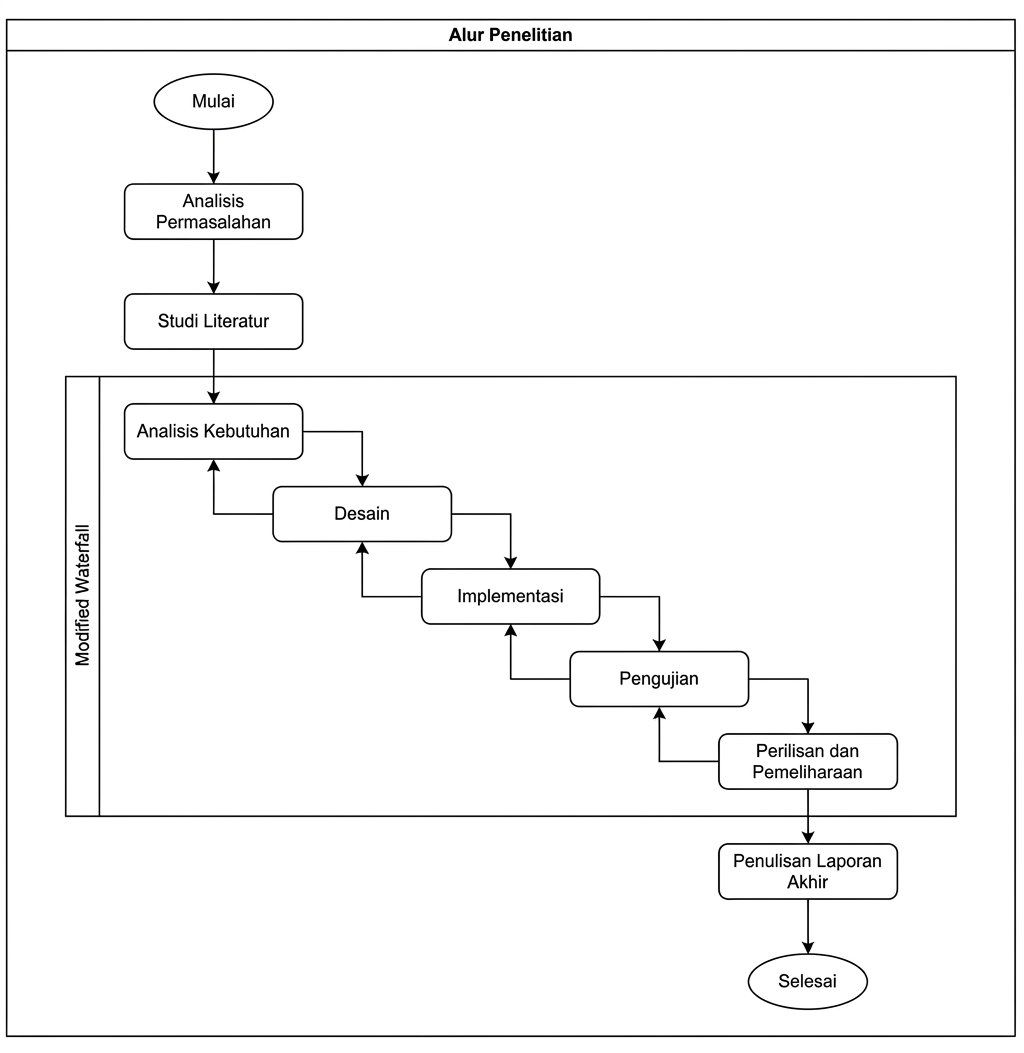
\includegraphics[width=0.95\textwidth]{figure/modified waterfall.png}
    \caption{Alur Penelitian dengan Model \textit{Modified Waterfall}}
    \label{fig:3.alur}
\end{figure}

Setiap tahapan dirancang secara berurutan dan saling berkaitan untuk memastikan proses penelitian berjalan secara sistematis dan terarah. Dalam penelitian ini, pengembangan sistem dilakukan menggunakan pendekatan \textit{Software Development Life Cycle} (SDLC) model \textit{Modified Waterfall} yang menjadi dasar dalam seluruh proses penelitian. Tahapan pengembangan sistem ini memungkinkan adanya penyesuaian pada tahap tertentu tanpa harus mengulang keseluruhan proses dari awal. \par

\section{Penjabaran Langkah Penelitian} \label{III.Penjabaran}
Setiap tahapan dalam alur penelitian memiliki peran yang saling mendukung untuk menghasilkan sistem yang sesuai dengan kebutuhan. Berikut merupakan penjabaran dari masing-masing tahapan yang dilakukan dalam penelitian ini.

\subsection{Analisis Permasalahan} \label{III.AnalisisPermasalahan}
Tahap ini merupakan titik awal penelitian, di mana peneliti mengidentifikasi permasalahan yang terjadi pada proses pelaporan kinerja unit di PT KAI Divre I Sumatera Utara. Identifikasi dilakukan melalui observasi langsung dan wawancara dengan pihak terkait, khususnya Manajer IT. Hasil dari tahap ini menjadi dasar dalam menentukan arah dan fokus penelitian secara keseluruhan. \par

\subsection{Studi Literatur} \label{III.StudiLiteratur}
Tahap studi literatur dilakukan untuk membangun landasan ilmiah yang kuat dalam mendukung proses perancangan dan pengembangan sistem. Kegiatan yang dilakukan pada tahap ini meliputi pencarian, pembacaan, dan pengkajian referensi yang relevan, mencakup jurnal ilmiah, buku, serta penelitian terdahulu yang berkaitan dengan topik penelitian. Referensi dikumpulkan dari sumber-sumber yang dapat dipertanggungjawabkan secara ilmiah dengan rentang waktu penerbitan minimal empat tahun terakhir untuk memastikan relevansi dan kemutakhiran informasi yang digunakan. Hasil dari tahap ini digunakan sebagai dasar teori dalam merancang sistem sekaligus sebagai pembanding untuk mengidentifikasi celah penelitian yang akan diselesaikan. \par

\subsection{Analisis Kebutuhan} \label{III.AnalisisKebutuhan}
Pada tahap ini, peneliti mengidentifikasi kebutuhan sistem secara menyeluruh berdasarkan hasil analisis permasalahan dan studi literatur yang telah dilakukan. Proses ini mencakup penentuan aktor sistem, kebutuhan fungsional, dan kebutuhan non-fungsional yang menjadi acuan dalam perancangan sistem. Apabila pada tahap selanjutnya ditemukan kebutuhan yang belum terakomodasi, tahap ini dapat ditinjau kembali sesuai karakteristik \textit{Modified Waterfall}. \par

\subsection{Desain Sistem} \label{III.DesainSistem}
Tahap desain mencakup perancangan arsitektur sistem, alur proses, struktur basis data, dan tampilan antarmuka yang akan digunakan oleh pengguna. Rancangan ini disusun berdasarkan hasil analisis kebutuhan agar seluruh kebutuhan pengguna dapat terakomodasi dengan baik sebelum proses implementasi dimulai. Jika pada tahap implementasi ditemukan ketidaksesuaian, desain dapat disesuaikan kembali tanpa harus mengulang dari awal. \par

\subsection{Implementasi} \label{III.Implementasi}
Tahap implementasi merupakan proses pembangunan sistem berdasarkan desain yang telah dibuat, mencakup pengembangan seluruh fitur seperti penginputan laporan, validasi berlapis, notifikasi otomatis, dasbor pemantauan, \textit{helpdesk}, dan ekspor laporan. Proses ini dilakukan secara bertahap dan modular agar setiap komponen dapat diuji secara mandiri sebelum diintegrasikan. Apabila ditemukan kendala selama pengembangan, penyesuaian dapat dilakukan dengan kembali ke tahap desain. \par

\subsection{Pengujian} \label{III.Pengujian}
Tahap pengujian dilakukan untuk memastikan sistem berjalan sesuai kebutuhan dan dapat diterima oleh pengguna. Pengujian dilakukan menggunakan \textit{blackbox testing} untuk memverifikasi fungsionalitas sistem dan \textit{User Acceptance Testing} (UAT) untuk mengukur tingkat keberterimaan sistem oleh pengguna di lingkungan PT KAI Divre I Sumatera Utara. Jika ditemukan kesalahan atau ketidaksesuaian, perbaikan dilakukan dengan kembali ke tahap implementasi. \par

\subsection{Perilisan dan Pemeliharaan} \label{III.Perilisan}
Setelah sistem dinyatakan layak melalui pengujian, sistem mulai dioperasikan dan dipantau kinerjanya dalam lingkungan nyata. Tahap ini bertujuan untuk memastikan sistem dapat berjalan stabil dan berkelanjutan sesuai kebutuhan operasional. Apabila ditemukan kendala setelah perilisan, perbaikan dilakukan untuk menjaga kestabilan sistem. \par

\subsection{Penulisan Laporan Akhir} \label{III.Laporan}
Tahap terakhir adalah penyusunan laporan penelitian sebagai dokumentasi menyeluruh dari seluruh proses yang telah dilakukan, mulai dari analisis permasalahan hingga hasil pengujian sistem. Laporan disusun secara sistematis sesuai pedoman yang berlaku agar hasil penelitian dapat dipahami dan dimanfaatkan oleh pihak-pihak yang berkepentingan. \par

\section{Alat dan Bahan Tugas Akhir} \label{III.AlatBahan}
Pada penelitian ini, alat dan bahan yang digunakan berperan penting dalam mendukung proses perancangan, pengembangan, hingga pengujian sistem. Pemilihan alat dan bahan disesuaikan dengan kebutuhan penelitian agar hasil yang diperoleh optimal.

\subsection{Alat} \label{III.Alat}
Alat yang digunakan dalam penelitian ini meliputi beberapa perangkat lunak pendukung sebagaimana ditunjukkan pada Tabel \ref{table:3.alat} berikut:

\begin{longtable}{|p{0.05\textwidth}|p{0.2\textwidth}|p{0.55\textwidth}|}
    \caption{Alat Penelitian}
    \label{table:3.alat}\\
    \hline
    \textbf{No} & \textbf{Alat} & \textbf{Fungsi} \\
    \hline
    \endfirsthead
    \multicolumn{3}{l}{\textit{Lanjutan dari halaman sebelumnya}} \\
    \caption[]{Alat Penelitian} \\
    \hline
    \textbf{No} & \textbf{Alat} & \textbf{Fungsi} \\
    \hline
    \endhead
    \hline
    \multicolumn{3}{r}{\textit{Bersambung ke halaman berikutnya}} \\
    \endfoot
    \endlastfoot
    1 & Visual Studio Code & \textit{Code editor} untuk menulis dan mengelola kode program \\
    \hline
    2 & Node.js & \textit{Runtime environment} untuk menjalankan aplikasi pada sisi \textit{server} \\
    \hline
    3 & Express.js & \textit{Framework backend} untuk membangun dan mengelola API sistem \\
    \hline
    4 & React.js & \textit{Frontend library} untuk membangun tampilan antarmuka berbasis web \\
    \hline
    5 & MySQL & Sistem manajemen basis data untuk menyimpan data sistem \\
    \hline
    6 & Prisma ORM & Penghubung aplikasi dengan basis data secara terstruktur \\
    \hline
    7 & Postman & Pengujian API yang telah dikembangkan \\
    \hline
    8 & Baileys & Integrasi sistem dengan WhatsApp Gateway \\
    \hline
    9 & Socket.io & Komunikasi data secara \textit{real-time} \\
    \hline
    10 & Figma & Perancangan tampilan antarmuka sebelum implementasi \\
    \hline
    11 & Draw.io & Pembuatan diagram alur dan rancangan sistem \\
    \hline
\end{longtable}

\subsection{Bahan} \label{III.Bahan}
Bahan yang digunakan dalam penelitian ini berupa data dan informasi yang mendukung proses analisis dan pengembangan sistem, sebagaimana ditunjukkan pada Tabel \ref{table:3.bahan} berikut:

\begin{longtable}{|p{0.05\textwidth}|p{0.25\textwidth}|p{0.15\textwidth}|p{0.35\textwidth}|}
    \caption{Bahan Penelitian}
    \label{table:3.bahan}\\
    \hline
    \textbf{No} & \textbf{Bahan} & \textbf{Jenis} & \textbf{Keterangan} \\
    \hline
    \endfirsthead
    \multicolumn{4}{l}{\textit{Lanjutan dari halaman sebelumnya}} \\
    \caption[]{Bahan Penelitian} \\
    \hline
    \textbf{No} & \textbf{Bahan} & \textbf{Jenis} & \textbf{Keterangan} \\
    \hline
    \endhead
    \hline
    \multicolumn{4}{r}{\textit{Bersambung ke halaman berikutnya}} \\
    \endfoot
    \endlastfoot
    1 & Hasil wawancara dengan Manajer IT PT KAI Divre I Sumatera Utara & Dataset pihak pertama & Diperoleh melalui wawancara langsung dengan Bapak Lexi Alexander sebagai dasar analisis kebutuhan sistem \\
    \hline
    2 & Format laporan harian unit KNA, Angkutan Penumpang, Angkutan Barang, dan Keuangan & Dataset pihak pertama & Diperoleh dari PT KAI Divre I Sumatera Utara sebagai acuan perancangan fitur penginputan dan validasi laporan \\
    \hline
    3 & Dokumen alur bisnis pelaporan kinerja unit & Dataset pihak pertama & Diperoleh melalui observasi langsung sebagai referensi dalam memahami proses pelaporan yang berjalan \\
    \hline
    4 & Kuesioner \textit{User Acceptance Testing} (UAT) & Dataset pihak pertama & Disusun sendiri dan diisi oleh pengguna sistem dari unit-unit terkait sebagai bahan pengujian keberterimaan sistem \\
    \hline
    5 & Jurnal dan referensi ilmiah & Dokumen panduan & Digunakan sebagai landasan teori dan pembanding dalam pengembangan sistem \\
    \hline
\end{longtable}

\section{Metode Pengembangan} \label{III.MetodePengembangan}
Subbab ini merupakan penjabaran lebih rinci dari setiap tahapan \textit{Modified Waterfall} yang telah digambarkan pada alur penelitian di Subbab \ref{III.Penjabaran}. Setiap tahapan diuraikan secara detail mulai dari analisis kebutuhan hingga perilisan sistem untuk memberikan gambaran yang jelas mengenai proses pengembangan yang dilakukan.

\subsection{Analisis Kebutuhan} \label{III.AnalisKebutuhan}
Tahap analisis kebutuhan bertujuan untuk mengidentifikasi kondisi sistem yang berjalan saat ini serta menentukan kebutuhan sistem yang akan dikembangkan secara menyeluruh. Pada tahap ini, kegiatan yang dilakukan meliputi identifikasi aktor sistem, pelaksanaan wawancara dengan pihak terkait, serta penyusunan kebutuhan fungsional dan non-fungsional sebagai acuan perancangan. Data dikumpulkan melalui observasi langsung dan wawancara dengan Manajer IT PT KAI Divre I Sumatera Utara untuk memperoleh gambaran nyata mengenai permasalahan dan kebutuhan yang ada. Seluruh hasil dari tahap ini kemudian didokumentasikan dan dijadikan dasar dalam tahap desain sistem. \par

\subsubsection*{a. Identifikasi Aktor Sistem}
Aktor sistem merupakan pihak yang berinteraksi langsung dengan sistem yang dikembangkan. Berdasarkan hasil analisis kebutuhan, terdapat tiga aktor dengan peran dan hak akses yang berbeda sebagaimana ditunjukkan pada Tabel \ref{table:3.aktor} berikut:

\begin{longtable}{|p{0.05\textwidth}|p{0.15\textwidth}|p{0.6\textwidth}|}
    \caption{Identifikasi Aktor Sistem}
    \label{table:3.aktor}\\
    \hline
    \textbf{No} & \textbf{Aktor} & \textbf{Peran dalam Sistem} \\
    \hline
    \endfirsthead
    \multicolumn{3}{l}{\textit{Lanjutan dari halaman sebelumnya}} \\
    \caption[]{Identifikasi Aktor Sistem} \\
    \hline
    \textbf{No} & \textbf{Aktor} & \textbf{Peran dalam Sistem} \\
    \hline
    \endhead
    \hline
    \multicolumn{3}{r}{\textit{Bersambung ke halaman berikutnya}} \\
    \endfoot
    \endlastfoot
    1 & User Unit & Menginput laporan harian, melakukan validasi internal, memantau status dan riwayat laporan unit masing-masing \\
    \hline
    2 & Admin Global & Melakukan validasi eksternal, mengulas dan menyetujui atau merevisi laporan, serta memantau kinerja seluruh unit melalui dasbor \\
    \hline
    3 & IT Support & Mengelola kendala teknis, menangani reset akun, serta memantau keamanan dan stabilitas sistem \\
    \hline
\end{longtable}

\subsubsection*{b. Pertanyaan Wawancara}
Pengumpulan data kebutuhan sistem dilakukan melalui proses wawancara dengan Bapak Lexi Alexander selaku Manajer IT PT KAI Divre I Sumatera Utara. Dokumen hasil wawancara merupakan kesimpulan yang disusun dari serangkaian diskusi dan komunikasi yang berlangsung secara bertahap, termasuk melalui percakapan langsung maupun daring. Dokumen tersebut kemudian dirangkum secara sistematis untuk keperluan analisis kebutuhan sistem. Berikut merupakan daftar pertanyaan yang digunakan sebagai panduan dalam proses wawancara:

\begin{longtable}{|p{0.05\textwidth}|p{0.2\textwidth}|p{0.55\textwidth}|}
    \caption{Daftar Pertanyaan Wawancara}
    \label{table:3.wawancara}\\
    \hline
    \textbf{No} & \textbf{Aspek} & \textbf{Pertanyaan} \\
    \hline
    \endfirsthead
    \multicolumn{3}{l}{\textit{Lanjutan dari halaman sebelumnya}} \\
    \caption[]{Daftar Pertanyaan Wawancara} \\
    \hline
    \textbf{No} & \textbf{Aspek} & \textbf{Pertanyaan} \\
    \hline
    \endhead
    \hline
    \multicolumn{3}{r}{\textit{Bersambung ke halaman berikutnya}} \\
    \endfoot
    \endlastfoot
    1 & Identitas Narasumber & Siapa nama, jabatan, dan peran narasumber dalam proses pelaporan? \\
    \hline
    2 & Proses Pelaporan & Bagaimana proses pelaporan yang berjalan saat ini di unit kerja? \\
    \hline
    3 & Proses Pelaporan & Seberapa sering laporan dikirim oleh masing-masing unit? \\
    \hline
    4 & Proses Pelaporan & Bagaimana alur setelah laporan dikirim oleh unit? \\
    \hline
    5 & Permasalahan & Apa kendala utama dalam proses pelaporan saat ini? \\
    \hline
    6 & Permasalahan & Apakah terjadi keterlambatan dalam pengiriman laporan? \\
    \hline
    7 & Dampak & Apa dampak dari keterlambatan tersebut terhadap operasional? \\
    \hline
    8 & Permasalahan & Apakah ada kendala lain yang sering terjadi dalam proses pelaporan? \\
    \hline
    9 & Alternatif Sistem & Apakah penggunaan Excel atau Google Form sudah cukup memadai? \\
    \hline
    10 & Alternatif Sistem & Apa keterbatasan Excel atau Google Form dari sisi kontrol akses? \\
    \hline
    11 & Alternatif Sistem & Apakah Excel atau Google Form mendukung alur validasi laporan? \\
    \hline
    12 & Alternatif Sistem & Bagaimana dengan ketersediaan notifikasi dan pemantauan \textit{real-time}? \\
    \hline
    13 & Alternatif Sistem & Apakah tersedia pencatatan aktivitas pengguna pada sistem yang ada? \\
    \hline
    14 & Kebutuhan Sistem & Apa yang paling dibutuhkan dari sistem yang akan dikembangkan? \\
    \hline
    15 & Kebutuhan Sistem & Apakah notifikasi otomatis diperlukan dalam sistem? \\
    \hline
    16 & Validasi & Bagaimana proses validasi laporan yang berjalan saat ini? \\
    \hline
    17 & Revisi & Bagaimana alur revisi laporan jika terdapat kesalahan? \\
    \hline
    18 & Data & Laporan berasal dari berapa unit dan apakah semua wajib melapor harian? \\
    \hline
    19 & Cakupan Penelitian & Mengapa penelitian difokuskan hanya pada 4 unit? \\
    \hline
    20 & Urgensi Sistem & Apakah sistem tetap diperlukan meskipun jumlah pengelola relatif sedikit? \\
    \hline
\end{longtable}

Berdasarkan hasil wawancara yang telah dilakukan dengan Bapak Lexi Alexander selaku Manajer IT PT KAI Divre I Sumatera Utara, diperoleh sejumlah temuan yang kemudian dianalisis untuk mengidentifikasi kebutuhan fungsional sistem. Pemetaan antara hasil wawancara dan kebutuhan fungsional yang dihasilkan dapat dilihat pada Tabel \ref{table:3.pemetaan-wawancara} berikut. \par

\begin{longtable}{|p{0.1\textwidth}|p{0.25\textwidth}|p{0.25\textwidth}|p{0.25\textwidth}|}
    \caption{Pemetaan Hasil Wawancara terhadap Kebutuhan Fungsional Sistem}
    \label{table:3.pemetaan-wawancara}\\
    \hline
    \textbf{No. Wwc} & \textbf{Temuan dari Jawaban Narasumber} & \textbf{Permasalahan yang Teridentifikasi} & \textbf{Kebutuhan Fungsional (F-ID)} \\
    \hline
    \endfirsthead
    \multicolumn{4}{l}{\textit{Lanjutan dari halaman sebelumnya}} \\
    \caption[]{Pemetaan Hasil Wawancara terhadap Kebutuhan Fungsional Sistem} \\
    \hline
    \textbf{No. Wwc} & \textbf{Temuan dari Jawaban Narasumber} & \textbf{Permasalahan yang Teridentifikasi} & \textbf{Kebutuhan Fungsional (F-ID)} \\
    \hline
    \endhead
    \hline
    \multicolumn{4}{r}{\textit{Bersambung ke halaman berikutnya}} \\
    \endfoot
    \endlastfoot
    2, 3, 4 & Pelaporan dilakukan melalui grup WhatsApp dengan format template chat, dikirim satu kali per hari, dan direkap manual oleh admin. & Tidak ada sistem terpusat untuk penginputan laporan harian per unit. & F-02 Input Laporan Harian \\
    \hline
    5, 11 & Format laporan tidak seragam dan data yang diinput langsung dianggap valid tanpa proses verifikasi atau mekanisme revisi terstruktur. & Tidak ada mekanisme validasi berlapis sebelum laporan dikirimkan. & F-03 Validasi Internal \newline F-04 Submit Laporan \\
    \hline
    4, 16, 17 & Admin membaca dan merekap laporan secara manual; feedback revisi diberikan melalui chat dan unit mengirim ulang laporan. & Tidak ada alur review laporan yang terstruktur oleh admin. & F-05 Validasi Eksternal (Review Admin) \\
    \hline
    8, 12, 14 & Laporan sering terlewat karena chat tenggelam di grup; tidak tersedia monitoring real-time; sistem terpusat dengan dashboard monitoring diperlukan. & Tidak ada dasbor pemantauan status laporan secara real-time. & F-06 Monitoring Dasbor \\
    \hline
    12, 15 & Tidak tersedia notifikasi otomatis; pengingat deadline dan informasi status laporan sangat diperlukan oleh unit maupun admin. & Keterlambatan laporan tidak dapat terdeteksi secara langsung tanpa notifikasi. & F-07 Notifikasi Otomatis (WhatsApp \& Real-time) \\
    \hline
    6, 17 & Beberapa unit terlambat menginput hingga beberapa hari; revisi dilakukan melalui chat dan menyebabkan double job. & Tidak ada mekanisme terpusat untuk penanganan revisi dan kendala teknis. & F-08 Helpdesk \\
    \hline
    10 & Excel maupun Google Form tidak memiliki pembatasan akses per unit secara spesifik, berpotensi menyebabkan data antar unit saling tercampur. & Akses data tidak terkontrol dan tidak dibatasi per unit/peran. & F-01 Login Sistem \newline F-09 Manajemen Akun dan Unit \\
    \hline
    13 & Tidak ada audit trail, sehingga perubahan data tidak dapat ditelusuri dan dipertanggungjawabkan. & Tidak ada pencatatan aktivitas pengguna yang dapat ditelusuri. & F-11 Audit Log \\
    \hline
    9, 20 & Sistem dengan server terpusat dibutuhkan untuk keamanan, kontrol data, serta scalable dan dapat di-handover ke pihak IT. & Sistem harus aman, mendukung multi-user, dan dapat dikembangkan. & F-01 Login \& Autentikasi JWT \newline F-10 Reset Password via Token \\
    \hline
    7, 19 & Keterlambatan laporan menyebabkan data tidak tercantum ke kantor pusat dan tidak dimasukkan ke pendapatan harian; 4 unit diprioritaskan karena terkait pendapatan. & Dibutuhkan perbandingan target vs realisasi untuk mendukung evaluasi kinerja. & F-12 Input Target \\
    \hline
\end{longtable}

\subsubsection*{c. Kebutuhan Fungsional Sistem}
Kebutuhan fungsional disusun berdasarkan hasil analisis dokumen wawancara secara menyeluruh. Setiap fungsi yang dirancang bertujuan langsung untuk mengatasi permasalahan yang ditemukan di lapangan, sebagaimana ditunjukkan pada Tabel \ref{table:3.fungsional} berikut:

\begin{longtable}{|p{0.1\textwidth}|p{0.25\textwidth}|p{0.5\textwidth}|}
    \caption{Kebutuhan Fungsional Sistem}
    \label{table:3.fungsional}\\
    \hline
    \textbf{ID} & \textbf{Kebutuhan} & \textbf{Keterangan} \\
    \hline
    \endfirsthead
    \multicolumn{3}{l}{\textit{Lanjutan dari halaman sebelumnya}} \\
    \caption[]{Kebutuhan Fungsional Sistem} \\
    \hline
    \textbf{ID} & \textbf{Kebutuhan} & \textbf{Keterangan} \\
    \hline
    \endhead
    \hline
    \multicolumn{3}{r}{\textit{Bersambung ke halaman berikutnya}} \\
    \endfoot
    \endlastfoot
    F-01 & Login sistem & Pengguna dapat masuk ke sistem menggunakan akun yang terdaftar dengan mekanisme keamanan pembatasan percobaan login \\
    \hline
    F-02 & Input laporan harian & User Unit dapat menginput laporan kinerja harian sesuai format masing-masing unit \\
    \hline
    F-03 & Validasi internal & User Unit dapat melakukan validasi laporan secara mandiri sebelum laporan dikirim ke Admin Global \\
    \hline
    F-04 & Submit laporan & Laporan hanya dapat dikirim ke Admin Global apabila telah melewati proses validasi internal \\
    \hline
    F-05 & Validasi eksternal & Admin Global dapat meninjau laporan yang masuk dan memberikan keputusan persetujuan atau revisi \\
    \hline
    F-06 & Monitoring dasbor & Admin Global dan User Unit dapat memantau status dan kinerja laporan melalui dasbor yang menyajikan data secara \textit{real-time} \\
    \hline
    F-07 & Notifikasi otomatis & Sistem mengirimkan notifikasi melalui WhatsApp dan Socket.io terkait status laporan, pengingat \textit{deadline}, dan informasi revisi \\
    \hline
    F-08 & Helpdesk & User Unit dapat mengajukan permintaan bantuan terkait kendala teknis, reset akun, maupun permintaan revisi laporan \\
    \hline
    F-09 & Manajemen akun dan unit & Admin Global dapat mengelola data akun pengguna dan unit kerja dalam sistem \\
    \hline
    F-10 & Reset password via token & IT Support dapat membangkitkan token \textit{one-time} untuk keperluan reset password pengguna yang akunnya terkunci \\
    \hline
    F-11 & Audit log & Sistem mencatat seluruh aktivitas pengguna sebagai jejak yang dapat ditelusuri \\
    \hline
    F-12 & Input target & User Unit dapat menginput target per periode sebagai dasar perbandingan dengan realisasi \\
    \hline
\end{longtable}

\subsubsection*{d. Kebutuhan Non-Fungsional Sistem}
Kebutuhan non-fungsional berkaitan dengan kualitas dan standar sistem secara keseluruhan di luar fungsionalitas utamanya. Berikut merupakan kebutuhan non-fungsional yang ditetapkan berdasarkan hasil analisis pada Tabel \ref{table:3.nonfungsional}:

\begin{longtable}{|p{0.1\textwidth}|p{0.2\textwidth}|p{0.55\textwidth}|}
    \caption{Kebutuhan Non-Fungsional Sistem}
    \label{table:3.nonfungsional}\\
    \hline
    \textbf{ID} & \textbf{Kebutuhan} & \textbf{Keterangan} \\
    \hline
    \endfirsthead
    \multicolumn{3}{l}{\textit{Lanjutan dari halaman sebelumnya}} \\
    \caption[]{Kebutuhan Non-Fungsional Sistem} \\
    \hline
    \textbf{ID} & \textbf{Kebutuhan} & \textbf{Keterangan} \\
    \hline
    \endhead
    \hline
    \multicolumn{3}{r}{\textit{Bersambung ke halaman berikutnya}} \\
    \endfoot
    \endlastfoot
    NF-01 & Keamanan & Sistem menerapkan autentikasi berbasis JWT, pembatasan hak akses per peran, serta mekanisme penguncian akun setelah tiga kali percobaan login yang gagal \\
    \hline
    NF-02 & Kinerja & Sistem mampu menampilkan dan memperbarui data secara cepat dan \textit{real-time} melalui Socket.io \\
    \hline
    NF-03 & Kemudahan Penggunaan & Sistem dirancang agar mudah digunakan oleh pengguna non-teknis sesuai dengan kebutuhan operasional harian \\
    \hline
    NF-04 & Keandalan & Sistem dapat berjalan secara stabil tanpa gangguan yang menghambat proses pelaporan \\
    \hline
    NF-05 & Kompatibilitas & Sistem dapat diakses melalui berbagai \textit{browser} pada perangkat \textit{desktop} maupun \textit{mobile} \\
    \hline
    NF-06 & Ketersediaan & Sistem dapat diakses kapan saja selama perangkat terhubung dengan jaringan internet \\
    \hline
\end{longtable}

\subsection{Desain Sistem} \label{III.Desain}
Tahap desain sistem merupakan kelanjutan dari tahap analisis yang telah menghasilkan gambaran kebutuhan secara menyeluruh. Pada tahap ini, kebutuhan-kebutuhan tersebut diterjemahkan ke dalam bentuk rancangan konkret yang dapat dijadikan acuan dalam proses implementasi. Desain sistem mencakup berbagai elemen visual dan struktural, mulai dari alur interaksi pengguna hingga rancangan antarmuka yang akan dibangun. Adapun cakupan desain sistem pada penelitian ini meliputi lima komponen utama, yaitu \textit{use case diagram}, \textit{activity diagram}, \textit{sequence diagram}, \textit{Entity Relationship Diagram} (ERD), serta desain antarmuka \textit{mid fidelity}. Setiap komponen memiliki peran dan fungsi masing-masing dalam menggambarkan sistem dari sudut pandang yang berbeda. \par

\subsubsection*{a. Use Case Diagram}
\textit{Use case diagram} merupakan salah satu jenis diagram dalam pemodelan sistem yang digunakan untuk menggambarkan interaksi antara pengguna dengan sistem secara fungsional. Diagram ini menunjukkan siapa saja aktor yang terlibat dalam sistem beserta fungsi-fungsi apa saja yang dapat mereka lakukan sesuai dengan kewenangannya masing-masing. Pada penelitian ini, \textit{use case diagram} disusun secara terpisah untuk setiap aktor guna memperjelas batasan hak akses dan tanggung jawab masing-masing peran dalam sistem. \par

Sebelum membaca diagram-diagram berikut, perlu ditegaskan bahwa seluruh proses pada sistem diasumsikan diawali dengan login terlebih dahulu. Dengan demikian, login diperlakukan sebagai prasyarat umum bagi setiap aktor dalam menjalankan fungsi sistem. \par

\begin{figure}[H]
    \centering
    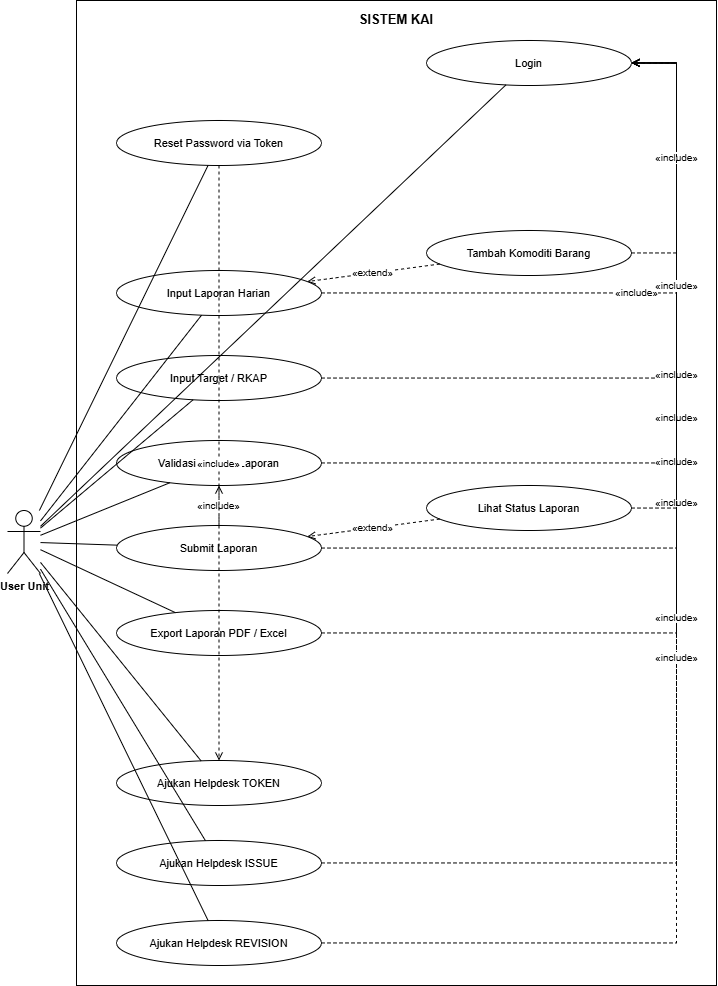
\includegraphics[width=0.85\textwidth]{figure/generated/usecase_user_unit.drawio (2).png}
    \caption{\textit{Use Case Diagram} Aktor User Unit}
    \label{fig:3.usecase-user-unit}
\end{figure}

Pada Gambar \ref{fig:3.usecase-user-unit} diatas adalah \textit{use case diagram} pertama yang menggambarkan interaksi User Unit dengan sistem yang mencakup fungsi Login, Reset Password via Token, Input Laporan Harian, Input Target/RKAP, Validasi Internal Laporan, Submit Laporan, Export Laporan PDF/Excel, Ajukan Helpdesk TOKEN, Ajukan Helpdesk ISSUE, dan Ajukan Helpdesk REVISION. Terdapat dua relasi tambahan pada diagram ini, yaitu fungsi Tambah Komoditi Barang yang bersifat \texttt{«extend»} terhadap Input Laporan Harian, serta fungsi Lihat Status Laporan yang bersifat \texttt{«extend»} terhadap Submit Laporan. Selain itu, fungsi Submit Laporan memiliki relasi \texttt{«include»} terhadap Validasi Internal Laporan, yang berarti proses validasi internal wajib dilalui sebelum laporan dapat di-\textit{submit}. \par
Gambar \ref{fig:3.usecase-user-unit} menunjukkan \textit{use case diagram} untuk aktor User Unit. Pada diagram ini, User Unit dapat berinteraksi dengan sistem melalui fungsi \textit{Login, Reset Password via Token, Input Laporan Harian, Input Target/RKAP, Validasi Internal Laporan, Submit Laporan, Export Laporan PDF/Excel}, serta pengajuan layanan \textit{helpdesk} (\textit{TOKEN, ISSUE}, dan \textit{REVISION}). Diagram ini juga memuat dua relasi \texttt{«extend»}, yaitu fungsi Tambah Komoditi Barang terhadap Input Laporan Harian dan fungsi Lihat Status Laporan terhadap Submit Laporan. Selain itu, terdapat relasi \texttt{«include»} pada fungsi Submit Laporan terhadap Validasi Internal Laporan, yang menegaskan bahwa proses validasi internal wajib dilalui sebelum laporan dapat dikirimkan kepada Admin Global. \par

\begin{figure}[H]
    \centering
    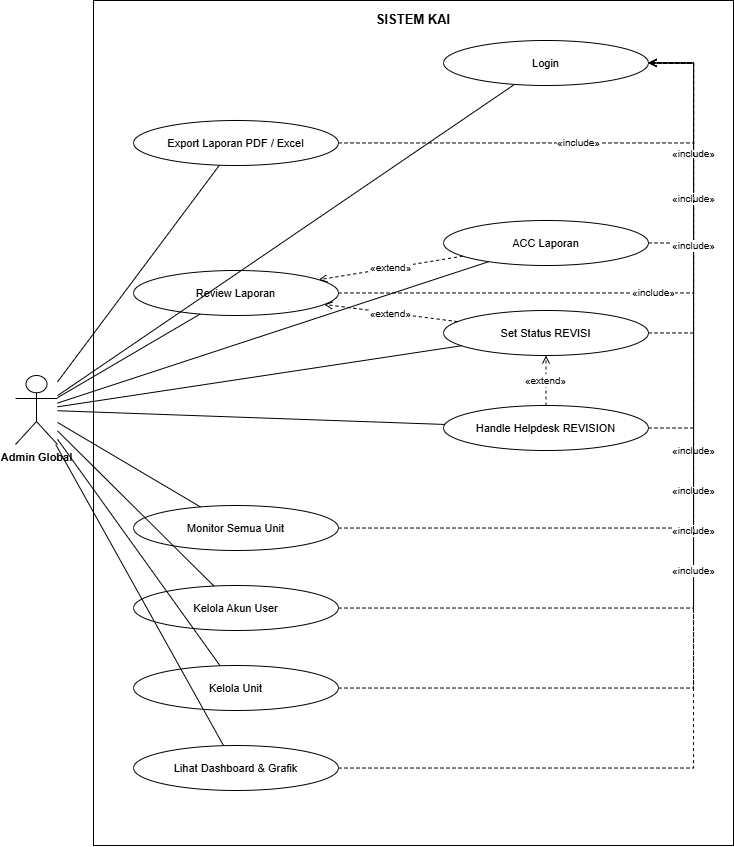
\includegraphics[width=0.85\textwidth]{figure/generated/usecase_admin_global.drawio (2).png}
    \caption{\textit{Use Case Diagram} Aktor Admin Global}
    \label{fig:3.usecase-admin-global}
\end{figure}
Pada Gambar \ref{fig:3.usecase-admin-global} diatas adalah \textit{Use case diagram} kedua yang menggambarkan interaksi Admin Global dengan sistem yang mencakup fungsi Login, Export Laporan PDF/Excel, Review Laporan, Monitor Semua Unit, Kelola Akun User, Kelola Unit, dan Lihat Dashboard \& Grafik. Fungsi ACC Laporan dan Set Status REVISI bersifat \texttt{«extend»} terhadap Review Laporan karena keduanya merupakan tindak lanjut yang dipilih setelah proses peninjauan dilakukan. Fungsi Handle Helpdesk REVISION memiliki relasi \texttt{«extend»} terhadap Set Status REVISI.\par
Gambar \ref{fig:3.usecase-admin-global} menunjukkan \textit{use case diagram} untuk aktor Admin Global. Aktor ini memiliki kewenangan untuk mengakses fungsi \textit{Login, Export Laporan PDF/Excel, Review Laporan, Monitor Semua Unit, Kelola Akun User, Kelola Unit}, serta \textit{Lihat Dashboard \& Grafik}. Pada fungsi Review Laporan, terdapat relasi \texttt{«extend»} dari fungsi ACC Laporan dan Set Status REVISI, yang merupakan opsi tindak lanjut setelah proses peninjauan dilakukan. Selain itu, fungsi Handle Helpdesk REVISION memiliki relasi \texttt{«extend»} terhadap Set Status REVISI, yang menandakan bahwa status revisi juga dapat dipicu melalui penanganan tiket bantuan dari User Unit. \par

\textit{Use case diagram} ketiga menggambarkan interaksi IT Support dengan sistem yang mencakup fungsi Login, Monitor Semua Unit, Handle Helpdesk TOKEN, dan Handle Helpdesk ISSUE. Fungsi Handle Helpdesk TOKEN memiliki relasi \texttt{«include»} terhadap Generate Token Reset Password, yang berarti setiap kali IT Support menangani tiket TOKEN, pembangkitan token reset password selalu menjadi bagian dari proses penanganannya. \textit{Use case diagram} aktor IT Support dapat dilihat pada Gambar \ref{fig:3.usecase-it-support} berikut. \par
Gambar \ref{fig:3.usecase-it-support} menunjukkan \textit{use case diagram} untuk aktor IT Support. Interaksi yang dapat dilakukan oleh aktor ini mencakup fungsi \textit{Login, Monitor Semua Unit, Handle Helpdesk TOKEN}, dan \textit{Handle Helpdesk ISSUE}. Pada penanganan tiket terkait akses akun, fungsi Handle Helpdesk TOKEN memiliki relasi \texttt{«include»} terhadap Generate Token Reset Password. Hal ini berarti bahwa setiap kali IT Support menangani tiket \textit{TOKEN}, proses pembangkitan token untuk pemulihan kata sandi selalu dieksekusi sebagai bagian dari penanganan tersebut. \par

\begin{figure}[H]
    \centering
    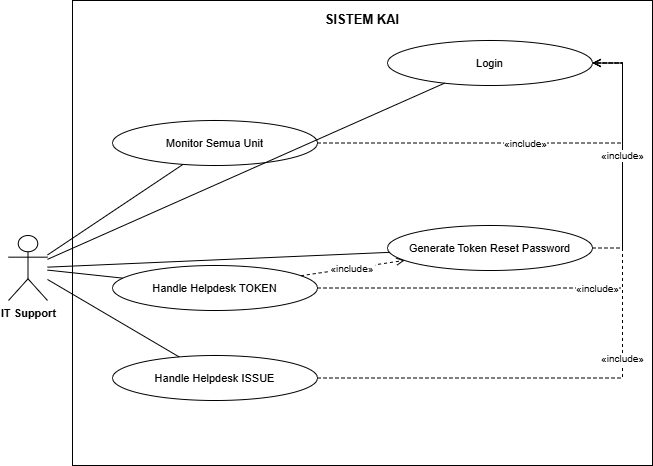
\includegraphics[width=0.85\textwidth]{figure/generated/usecase_it_support.drawio (2).png}
    \caption{\textit{Use Case Diagram} Aktor IT Support}
    \label{fig:3.usecase-it-support}
\end{figure}

\subsubsection*{b. Activity Diagram}
\textit{Activity diagram} digunakan untuk menggambarkan alur kerja atau proses yang terjadi di dalam sistem secara lebih rinci dibandingkan \textit{use case diagram}. Diagram ini menjelaskan urutan aktivitas yang dilakukan oleh setiap aktor beserta keputusan-keputusan yang terjadi di setiap titik alur. Pada sistem ini, terdapat enam \textit{activity diagram} yang masing-masing merepresentasikan satu proses utama yang berjalan dalam sistem. \par
\textbf{Activity Diagram 1: Login \& Mekanisme Lock Akun.}\par
\begin{figure}[H]
    \centering
    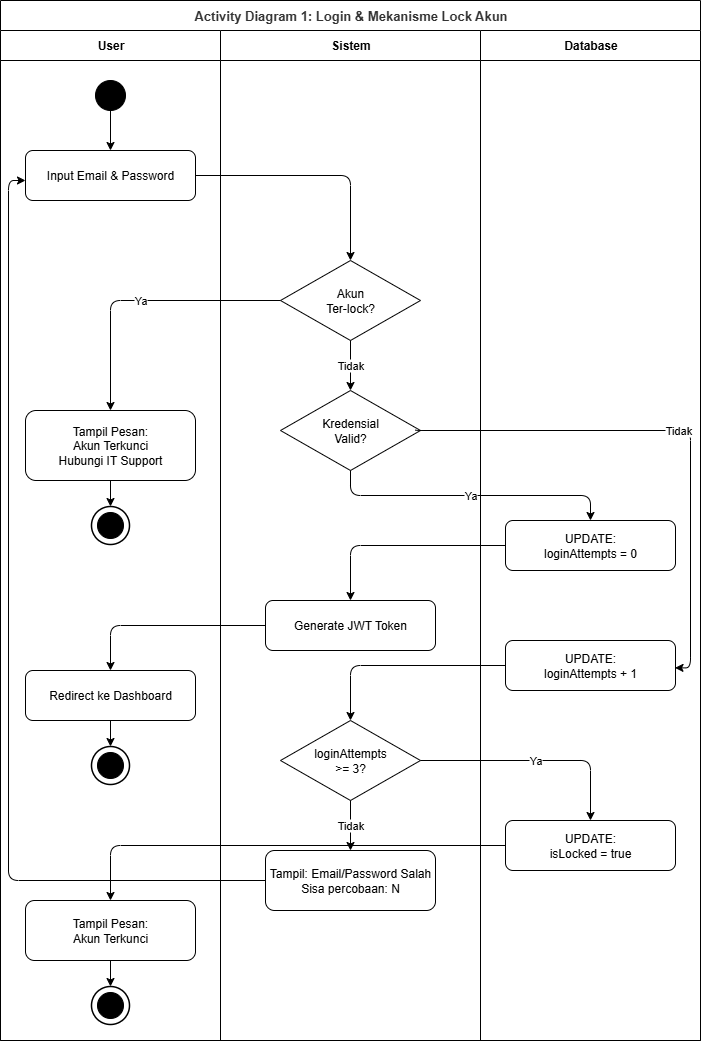
\includegraphics[width=0.85\textwidth]{figure/activity_png/activity_1_login.drawio.png}
    \caption{\textit{Activity Diagram} 1: Login \& Mekanisme Lock Akun}
    \label{fig:3.ad-login}
\end{figure}

Alur proses login beserta mekanisme penguncian akun ini dapat dilihat pada Gambar \ref{fig:3.ad-login} diatas .Proses autentikasi merupakan pintu masuk utama bagi seluruh pengguna sistem sebelum dapat mengakses fitur-fitur yang tersedia. Sistem dirancang dengan mekanisme keamanan berlapis di mana setiap percobaan login yang gagal akan dicatat dan diakumulasikan oleh sistem. Apabila pengguna gagal melakukan login sebanyak tiga kali secara berturut-turut, akun akan dikunci secara otomatis oleh sistem untuk mencegah akses yang tidak sah. \par

Berdasarkan \textit{activity diagram} pada Gambar \ref{fig:3.ad-login}, alur dimulai ketika pengguna memasukkan email dan kata sandi, kemudian sistem memeriksa apakah akun dalam kondisi terkunci. Jika terkunci, sistem langsung menampilkan pesan untuk menghubungi IT Support tanpa melanjutkan proses verifikasi. Jika tidak terkunci, sistem memvalidasi kredensial; apabila valid, JWT token dibangkitkan dan pengguna diarahkan ke \textit{dashboard}, sedangkan apabila tidak valid, nilai \texttt{loginAttempts} bertambah satu. Apabila jumlah kegagalan telah mencapai tiga kali, sistem secara otomatis mengunci akun dan menampilkan pesan akun terkunci kepada pengguna. \par

\textbf{Activity Diagram 2: Reset Password via Token.} \par

Pengguna yang akunnya terkunci tidak dapat langsung memulihkan akses secara mandiri, melainkan harus melalui proses bantuan yang melibatkan IT Support. Proses ini dirancang untuk menjaga keamanan sistem sekaligus memastikan bahwa hanya pengguna yang sah yang dapat memulihkan akses akunnya. Mekanisme pemulihan menggunakan token satu kali pakai yang memiliki batas waktu kedaluwarsa selama satu jam. Alur proses reset password via token ini dapat dilihat pada Gambar \ref{fig:3.ad-reset} berikut. \par

\begin{figure}[H]
    \centering
    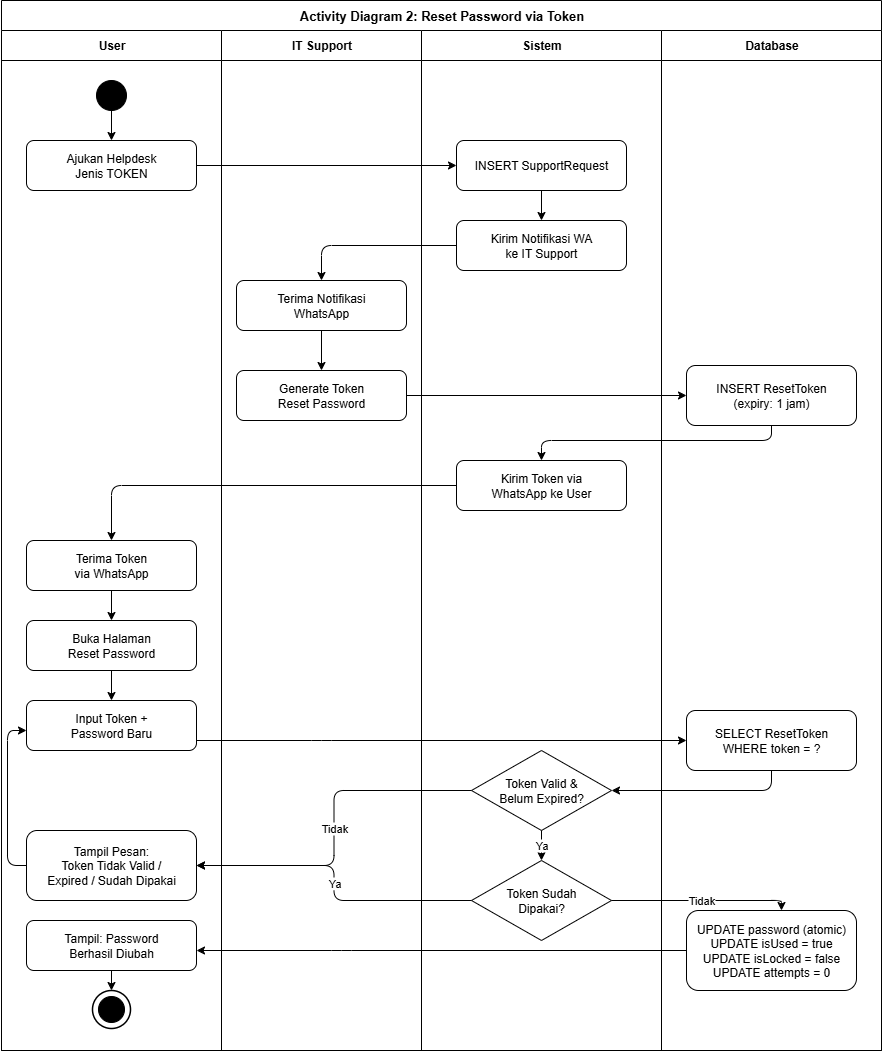
\includegraphics[width=0.95\textwidth]{figure/activity_png/activity_2_reset_password.drawio.png}
    \caption{\textit{Activity Diagram} 2: Reset Password via Token}
    \label{fig:3.ad-reset}
\end{figure}

Berdasarkan \textit{activity diagram} pada Gambar \ref{fig:3.ad-reset}, proses diawali dengan pengguna mengajukan \textit{helpdesk} jenis TOKEN, lalu sistem mengirimkan notifikasi WhatsApp kepada IT Support untuk ditindaklanjuti. IT Support memverifikasi identitas pengguna dan membangkitkan token yang dikirimkan kembali kepada pengguna melalui WhatsApp. Pengguna kemudian membuka halaman reset password dan memasukkan token beserta kata sandi baru; sistem memvalidasi token tersebut dan apabila valid serta belum digunakan, sistem memperbarui kata sandi secara \textit{atomic} sekaligus membuka kunci akun pengguna. \par

\textbf{Activity Diagram 3: Input Laporan \& Validasi Internal.} \par
\begin{figure}[H]
    \centering
    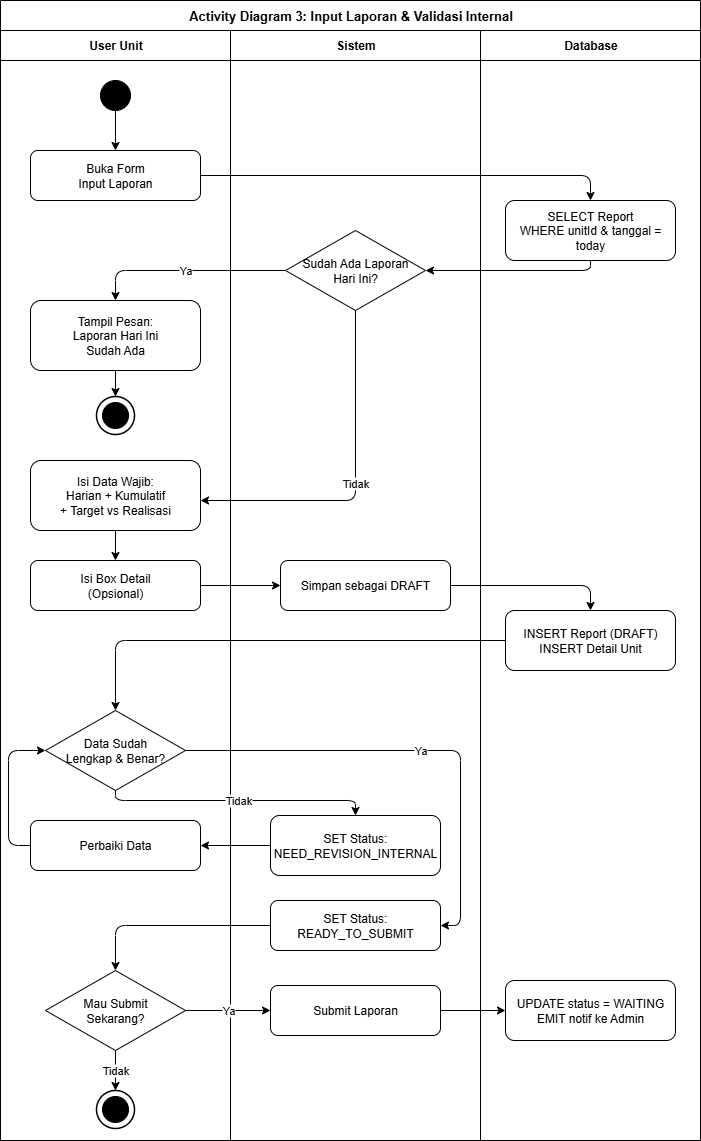
\includegraphics[width=0.85\textwidth]{figure/activity_png/activity_3_input_laporan.drawio.png}
    \caption{\textit{Activity Diagram} 3: Input Laporan \& Validasi Internal}
    \label{fig:3.ad-input}
\end{figure}
Alur proses penginputan laporan dan validasi internal ini dapat dilihat pada Gambar \ref{fig:3.ad-input} diatas.Penginputan laporan harian merupakan fungsi inti yang dijalankan oleh User Unit setiap hari kerja sebagai bentuk pertanggungjawaban kinerja unit masing-masing. Sistem menerapkan batasan satu laporan per unit per hari untuk menjaga konsistensi dan integritas data pelaporan. Sebelum laporan dapat dikirimkan kepada Admin Global, laporan tersebut harus terlebih dahulu melewati proses validasi internal yang dilakukan oleh User Unit itu sendiri. \par

Berdasarkan \textit{activity diagram} pada Gambar \ref{fig:3.ad-input}, sistem terlebih dahulu memeriksa apakah laporan untuk unit dan tanggal hari ini sudah ada; jika sudah, proses langsung berakhir dengan pesan informasi kepada pengguna. Apabila belum ada, pengguna mengisi data wajib dan secara opsional mengisi \textit{box} detail, kemudian laporan disimpan dengan status DRAFT. Sistem memeriksa kelengkapan data; jika belum lengkap, status diubah menjadi \texttt{NEED\allowbreak\_REVISION\allowbreak\_INTERNAL} dan pengguna diminta memperbaiki isian, sedangkan jika sudah valid, status diperbarui menjadi \texttt{READY\allowbreak\_TO\allowbreak\_SUBMIT}. Pada kondisi \texttt{READY\allowbreak\_TO\allowbreak\_SUBMIT}, pengguna dapat langsung melakukan \textit{submit} sehingga status laporan berubah menjadi WAITING dan notifikasi dikirimkan kepada Admin Global. \par


\textbf{Activity Diagram 4: Admin Review Laporan (ACC / REVISI).} \par
Setelah laporan berhasil di-\textit{submit} oleh User Unit, proses selanjutnya berada di tangan Admin Global yang bertugas meninjau dan memberikan keputusan atas setiap laporan yang masuk. Admin Global dapat memberikan dua jenis keputusan, yaitu ACC apabila laporan sudah sesuai, atau REVISI apabila laporan perlu diperbaiki kembali oleh unit terkait. Setiap keputusan yang diambil akan dicatat dalam sistem melalui mekanisme \textit{audit log} untuk keperluan keterlacakan. Alur proses review laporan oleh Admin Global dapat dilihat pada Gambar \ref{fig:3.ad-review}. \par

Berdasarkan \textit{activity diagram} pada Gambar \ref{fig:3.ad-review}, Admin Global membuka \textit{dashboard} dan sistem menampilkan seluruh laporan berstatus WAITING untuk ditinjau. Admin Global membaca detail laporan lalu mengambil keputusan; apabila laporan sudah sesuai, Admin Global mengeklik ACC sehingga status laporan diperbarui dan notifikasi \textit{real-time} dikirimkan kepada User Unit. Apabila laporan perlu diperbaiki, Admin Global mengisi catatan revisi dan mengeklik REVISI, sehingga sistem memperbarui status laporan dan mengirimkan notifikasi melalui WhatsApp sekaligus \textit{real-time} kepada User Unit. Seluruh keputusan yang diambil, baik ACC maupun REVISI, dicatat secara otomatis ke dalam AuditLog oleh sistem. \par

\begin{figure}[H]
    \centering
    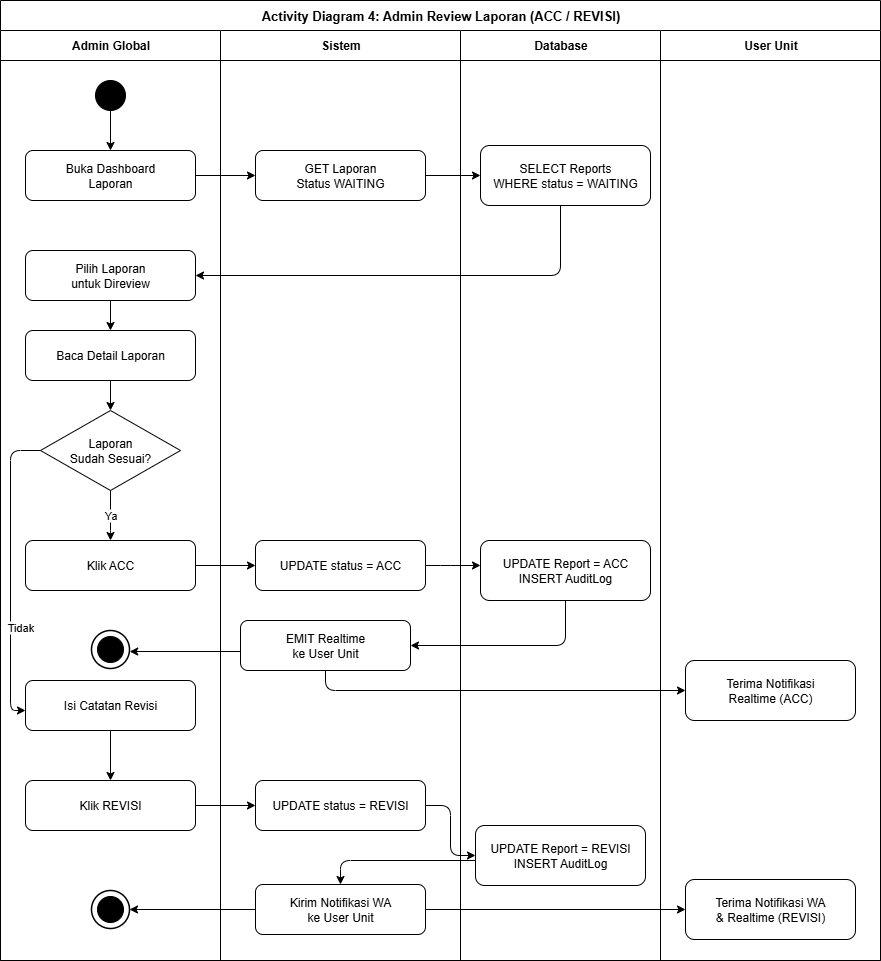
\includegraphics[width=0.95\textwidth]{figure/activity_png/activity_4_admin_review.drawio.png}
    \caption{\textit{Activity Diagram} 4: Admin Review Laporan (ACC / REVISI)}
    \label{fig:3.ad-review}
\end{figure}

\textbf{Activity Diagram 5: Edit Laporan Setelah Submit (via Helpdesk REVISION).} \par
\begin{figure}[H]
    \centering
    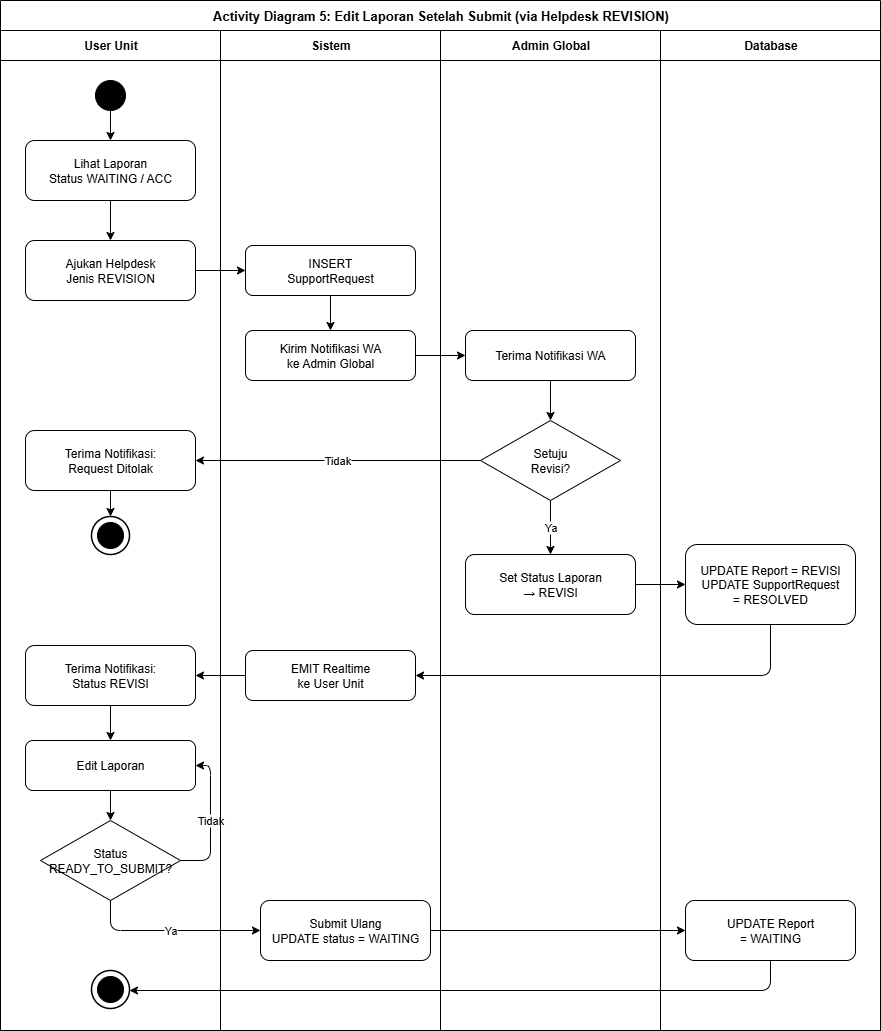
\includegraphics[width=0.95\textwidth]{figure/activity_png/activity_5_edit_helpdesk.drawio.png}
    \caption{\textit{Activity Diagram} 5: Edit Laporan Setelah Submit (via Helpdesk REVISION)}
    \label{fig:3.ad-edit}
\end{figure}
Alur proses edit laporan setelah \textit{submit} melalui \textit{helpdesk} ini dapat dilihat pada Gambar \ref{fig:3.ad-edit} diatas.Sistem memberlakukan aturan bahwa laporan yang telah di-\textit{submit} tidak dapat diubah secara langsung oleh User Unit tanpa melalui mekanisme yang telah ditetapkan. Hal ini bertujuan untuk menjaga integritas dan akuntabilitas data laporan yang telah masuk ke dalam sistem. Apabila User Unit perlu melakukan perubahan terhadap laporan yang sudah berstatus WAITING atau ACC, maka harus mengajukan permintaan melalui sistem \textit{helpdesk} jenis REVISION. \par

Berdasarkan \textit{activity diagram} pada Gambar \ref{fig:3.ad-edit}, User Unit mengajukan \textit{helpdesk} jenis REVISION dan sistem mengirimkan notifikasi WhatsApp kepada Admin Global untuk ditindaklanjuti. Admin Global mengevaluasi permintaan; apabila tidak disetujui, notifikasi penolakan dikirimkan kepada User Unit dan proses berakhir, sedangkan apabila disetujui, status laporan diubah menjadi REVISI dan User Unit menerima notifikasi \textit{real-time}. User Unit kemudian melakukan perbaikan laporan hingga statusnya mencapai \texttt{READY\allowbreak\_TO\allowbreak\_SUBMIT}, lalu melakukan \textit{submit} ulang sehingga status laporan kembali menjadi WAITING untuk ditinjau kembali oleh Admin Global. \par

% \begin{figure}[H]
%     \centering
%     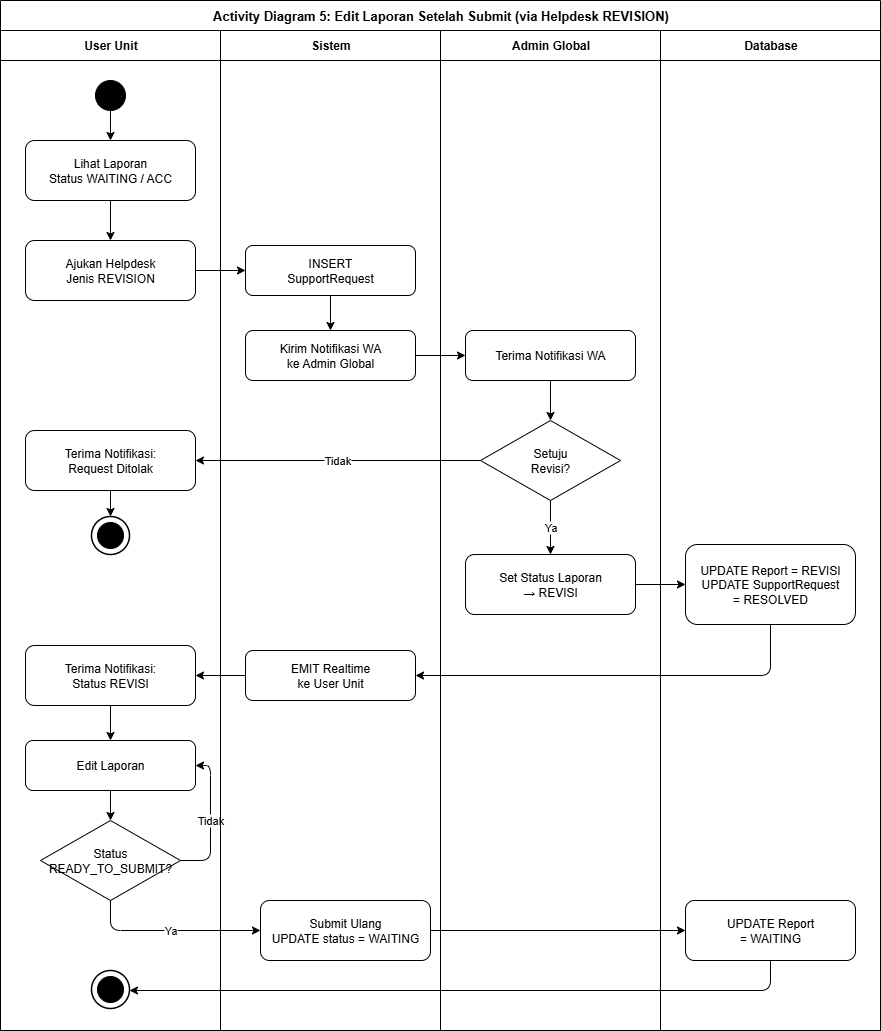
\includegraphics[width=0.95\textwidth]{figure/activity_png/activity_5_edit_helpdesk.drawio.png}
%     \caption{\textit{Activity Diagram} 5: Edit Laporan Setelah Submit (via Helpdesk REVISION)}
%     \label{fig:3.ad-edit}
% \end{figure}

\textbf{Activity Diagram 6: Sistem Helpdesk (TOKEN / ISSUE / REVISION).} \par
Sistem \textit{helpdesk} dirancang sebagai mekanisme terpusat untuk menangani berbagai kendala yang dialami pengguna selama menggunakan sistem, mulai dari masalah akses akun hingga permintaan perubahan data laporan. Setiap permintaan yang masuk diklasifikasikan ke dalam salah satu dari tiga jenis tiket dan secara otomatis diteruskan kepada pihak yang berwenang menanganinya. Dengan adanya sistem ini, pengguna tidak perlu melakukan komunikasi di luar sistem untuk melaporkan kendala yang dialami. Alur kerja lengkap sistem \textit{helpdesk} untuk ketiga jenis tiket dapat dilihat pada Gambar \ref{fig:3.ad-helpdesk}. \par

Berdasarkan \textit{activity diagram} pada Gambar \ref{fig:3.ad-helpdesk}, pengguna mengajukan \textit{helpdesk} dengan memilih jenis tiket dan mengisi deskripsi kendala, kemudian sistem menyimpan permintaan dan meneruskannya sesuai jenisnya. Tiket TOKEN diteruskan ke IT Support untuk proses verifikasi identitas dan pembangkitan token \textit{reset password} yang dikirim melalui WhatsApp, sehingga pengguna dapat memulihkan akses akunnya. Tiket ISSUE diteruskan ke IT Support untuk investigasi teknis, dan setelah kendala diselesaikan, pengguna menerima notifikasi \textit{real-time} bahwa masalahnya telah ditangani. Tiket REVISION diteruskan ke Admin Global yang kemudian mengubah status laporan terkait menjadi REVISI melalui \textit{dashboard}, dan pengguna menerima notifikasi untuk segera melakukan perbaikan. \par

\begin{figure}[H]
    \centering
    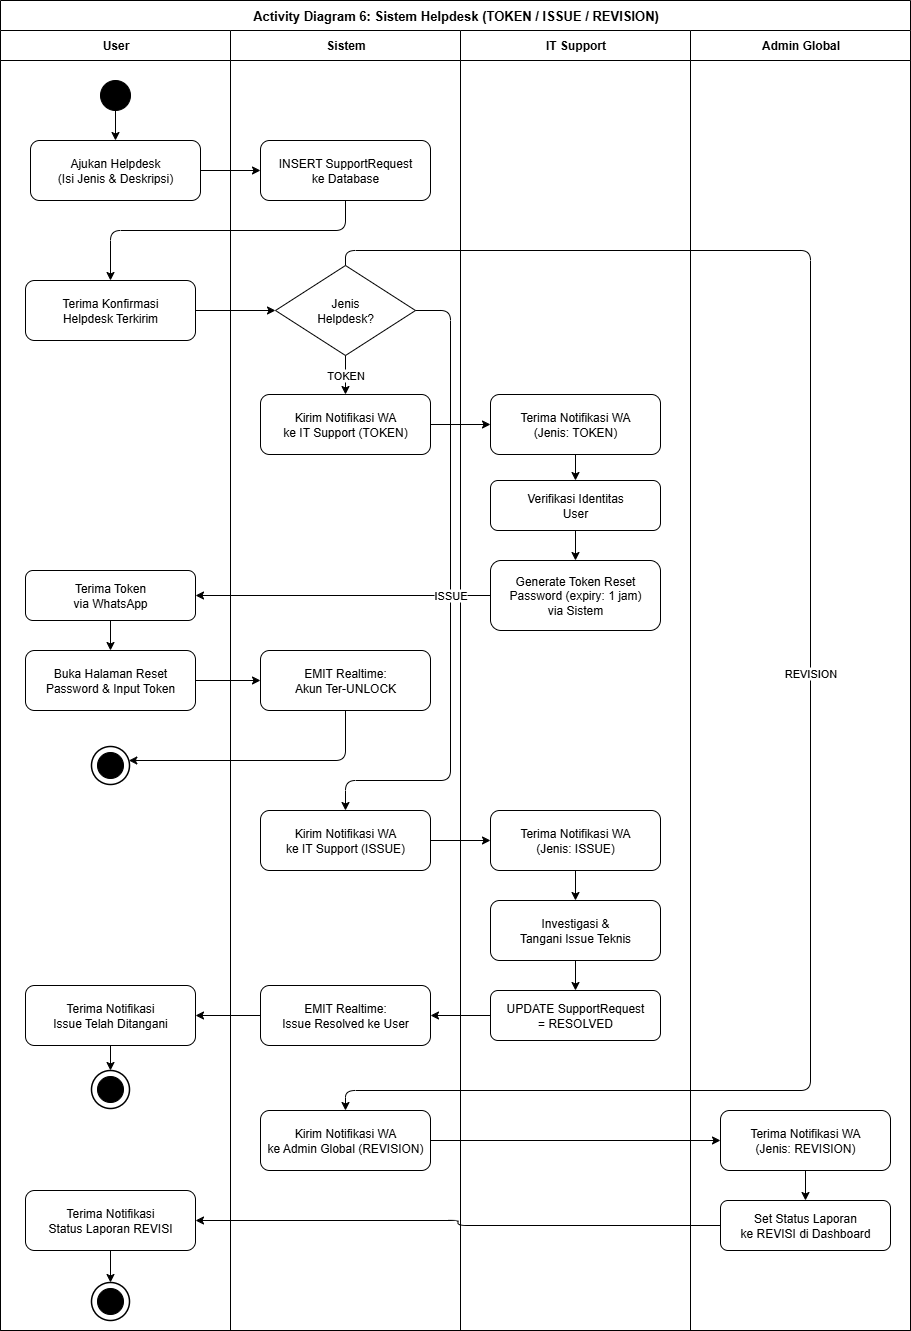
\includegraphics[width=0.95\textwidth]{figure/activity_png/activity_6_helpdesk.drawio.png}
    \caption{\textit{Activity Diagram} 6: Sistem Helpdesk (TOKEN / ISSUE / REVISION)}
    \label{fig:3.ad-helpdesk}
\end{figure}

\FloatBarrier
\subsubsection*{c. Sequence Diagram}
\textit{Sequence diagram} digunakan untuk menggambarkan urutan pertukaran pesan antar komponen sistem dalam menjalankan suatu proses tertentu. Berbeda dengan \textit{activity diagram} yang berfokus pada alur aktivitas, \textit{sequence diagram} lebih menitikberatkan pada bagaimana setiap komponen , mulai dari \textit{frontend}, \textit{backend}, \textit{database}, hingga layanan eksternal, saling berkomunikasi secara berurutan. Pada sistem ini terdapat lima \textit{sequence diagram} yang merepresentasikan proses-proses utama dalam sistem. \par

\textbf{Sequence Diagram 1: Login \& Mekanisme Lock Akun.} \par
Proses login melibatkan komunikasi berurutan antara empat komponen utama, yaitu User, Frontend (React), Backend (Express), dan Database (MySQL). Setiap permintaan login yang masuk diproses secara bertahap mulai dari sisi klien hingga ke lapisan basis data sebelum respons dikembalikan. Alur komunikasi antar komponen dalam proses login dan mekanisme penguncian akun ini dapat dilihat pada Gambar \ref{fig:3.seq-login}. \par

Berdasarkan \textit{sequence diagram} pada Gambar \ref{fig:3.seq-login}, pengguna memasukkan email dan kata sandi pada \textit{frontend} yang kemudian mengirimkan permintaan \texttt{POST /api/auth/login} ke \textit{backend}. \textit{Backend} mengambil data pengguna dari \textit{database} dan memeriksa kondisi akun; apabila akun terkunci, \textit{backend} langsung mengembalikan respons 403 dan \textit{frontend} menampilkan pesan untuk menghubungi IT Support. Apabila kredensial salah, \textit{backend} memperbarui nilai \texttt{loginAttempts} dan jika sudah mencapai tiga kali, status \texttt{isLocked} diubah menjadi \texttt{true} sehingga \textit{frontend} menampilkan pesan akun terkunci. Apabila kredensial benar, \textit{backend} mereset \texttt{loginAttempts} menjadi nol, membangkitkan JWT token, dan mengembalikan respons 200 sehingga \textit{frontend} menyimpan token dan mengarahkan pengguna ke \textit{dashboard}. \par

\begin{figure}[H]
    \centering
    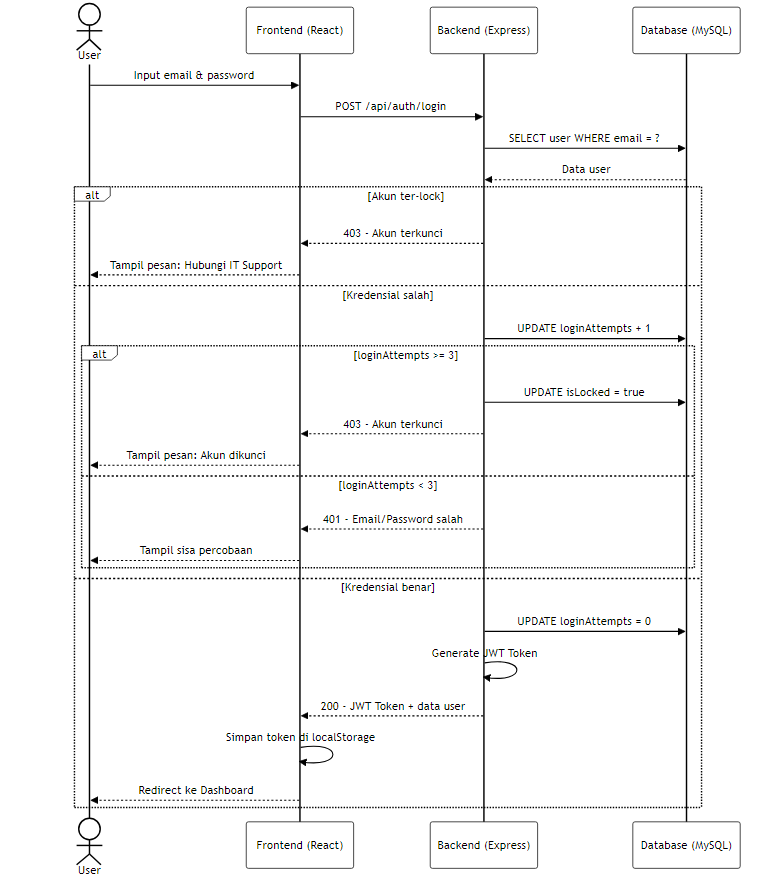
\includegraphics[width=0.95\textwidth]{figure/sequence-login.png}
    \caption{\textit{Sequence Diagram} 1: Login \& Mekanisme Lock Akun}
    \label{fig:3.seq-login}
\end{figure}

\textbf{Sequence Diagram 2: Reset Password via Token.}\par
Proses reset password melibatkan lima komponen yang saling berkomunikasi, yaitu User Unit, IT Support, Frontend, Backend, Database, dan layanan WhatsApp melalui Baileys. Kompleksitas proses ini mencerminkan pentingnya keamanan dalam pemulihan akses akun pengguna yang terkunci. Alur komunikasi antar komponen dalam proses reset password via token ini dapat dilihat pada Gambar \ref{fig:3.seq-reset}. \par

Berdasarkan \textit{sequence diagram} pada Gambar \ref{fig:3.seq-reset}, pengguna mengajukan \textit{helpdesk} jenis TOKEN melalui \textit{frontend} yang mengirimkan \texttt{POST /api/helpdesk} ke \textit{backend}, kemudian \textit{backend} menyimpan SupportRequest ke \textit{database} dan mengirimkan notifikasi WhatsApp kepada IT Support. IT Support membuka tiket lalu meminta sistem membangkitkan token melalui \texttt{POST /api/token/generate}, di mana \textit{backend} menyimpan ResetToken ke \textit{database} dan mengirimkan token tersebut ke nomor WhatsApp pengguna. Pengguna memasukkan token dan kata sandi baru melalui \texttt{POST /api/auth/reset-password}; apabila token tidak valid atau sudah kedaluwarsa, \textit{backend} mengembalikan respons 400 dan \textit{frontend} menampilkan pesan kesalahan. Apabila token valid, \textit{backend} memperbarui kata sandi secara \textit{atomic}, menandai token sebagai sudah dipakai, membuka kunci akun, dan mengembalikan respons 200 sehingga pengguna diarahkan kembali ke halaman login. \par

\begin{figure}[H]
    \centering
    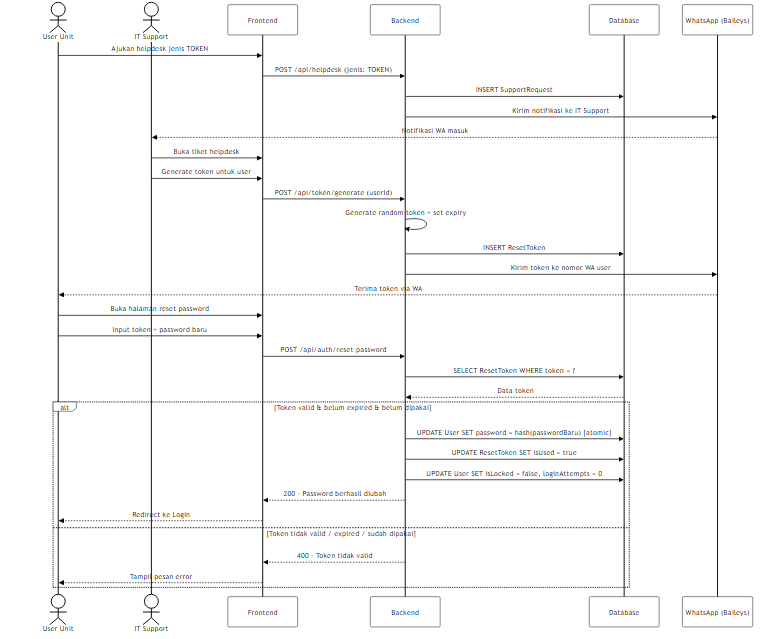
\includegraphics[width=0.95\textwidth]{figure/sequence-reset-password.png}
    \caption{\textit{Sequence Diagram} 2: Reset Password via Token}
    \label{fig:3.seq-reset}
\end{figure}

\textbf{Sequence Diagram 3: Submit Laporan.}\par
Proses submit laporan melibatkan komunikasi antara User Unit, Frontend, Backend, Database, dan Socket.io sebagai layanan notifikasi \textit{real-time}. Proses ini mencakup tiga tahapan utama, yaitu pengecekan laporan harian, penginputan data, validasi internal, hingga pengiriman laporan. Alur komunikasi antar komponen dalam proses submit laporan ini dapat dilihat pada Gambar \ref{fig:3.seq-submit} berikut. \par
\begin{figure}[H]
    \centering
    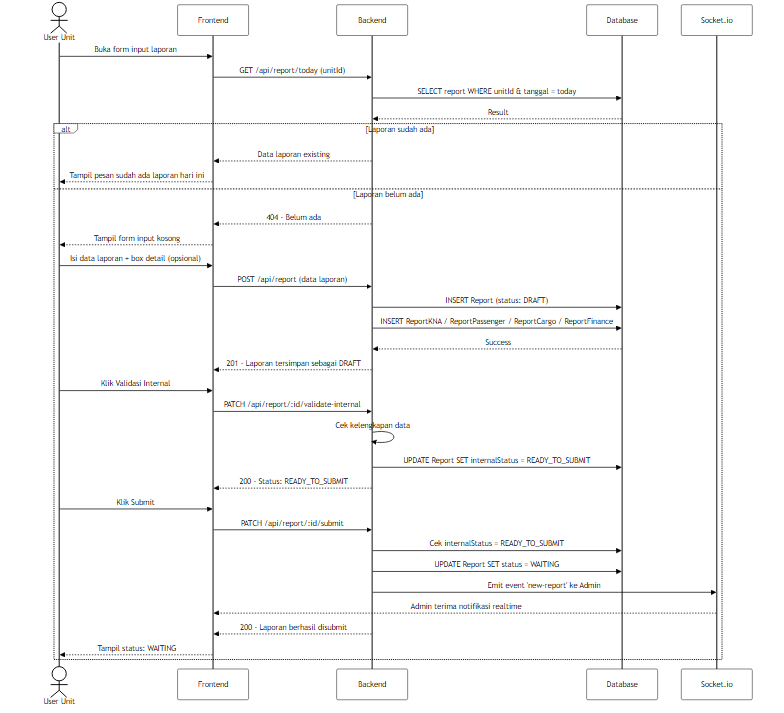
\includegraphics[width=0.95\textwidth]{figure/sequence-submit-laporan.png}
    \caption{\textit{Sequence Diagram} 3: Submit Laporan}
    \label{fig:3.seq-submit}
\end{figure}
Berdasarkan \textit{sequence diagram} pada Gambar \ref{fig:3.seq-submit}, \textit{frontend} terlebih dahulu mengirimkan \texttt{GET /api/report/today} ke \textit{backend} untuk memeriksa keberadaan laporan hari ini; apabila sudah ada, \textit{backend} mengembalikan data laporan \textit{existing} dan \textit{frontend} menampilkan pesan bahwa laporan hari ini telah dibuat. Apabila belum ada, \textit{frontend} menampilkan formulir kosong dan pengguna mengisi data laporan, kemudian mengirimkan \texttt{POST /api/report} sehingga \textit{backend} menyimpan laporan beserta detail unitnya ke \textit{database} dengan status DRAFT. Pengguna mengeklik tombol validasi internal yang mengirimkan \texttt{PATCH /api/report/:id/validate-internal} dan \textit{backend} memperbarui status menjadi \texttt{READY\allowbreak\_TO\allowbreak\_SUBMIT}. Pengguna kemudian mengeklik \textit{submit} melalui \texttt{PATCH /api/report/:id/submit} dan \textit{backend} memperbarui status menjadi WAITING sekaligus mengirimkan \textit{event} \texttt{new-report} melalui Socket.io sehingga Admin Global menerima notifikasi \textit{real-time}. \par

\textbf{Sequence Diagram 4: Admin Review Laporan (ACC / REVISI).}\par
Proses review laporan oleh Admin Global melibatkan komunikasi antara Admin Global, User Unit, Frontend, Backend, Database, Socket.io, dan layanan WhatsApp melalui Baileys. Setiap keputusan yang diambil Admin Global menghasilkan respons yang berbeda baik di sisi sistem maupun di sisi penerima notifikasi. Alur komunikasi antar komponen dalam proses review laporan ini dapat dilihat pada Gambar \ref{fig:3.seq-review}. \par

Berdasarkan \textit{sequence diagram} pada Gambar \ref{fig:3.seq-review}, Admin Global membuka daftar laporan melalui \texttt{GET /api/report?status=WAITING} dan \textit{backend} mengambil seluruh laporan berstatus WAITING dari \textit{database} untuk ditampilkan. Admin Global membuka detail laporan melalui \texttt{GET /api/report/:id} kemudian mengambil keputusan; apabila ACC, \textit{frontend} mengirimkan \texttt{PATCH /api/report/:id/review} dengan status ACC, lalu \textit{backend} memperbarui status laporan, mencatat ke AuditLog, dan mengirimkan \textit{event} melalui Socket.io sehingga User Unit menerima notifikasi \textit{real-time}. Apabila REVISI, Admin Global mengisi catatan revisi dan \textit{backend} memperbarui status laporan menjadi REVISI, mencatat ke AuditLog, mengirimkan \textit{event} Socket.io, sekaligus mengirimkan notifikasi WhatsApp kepada User Unit. User Unit pun menerima pemberitahuan melalui dua kanal sekaligus, yaitu notifikasi \textit{real-time} di sistem dan pesan WhatsApp. \par

\begin{figure}[H]
    \centering
    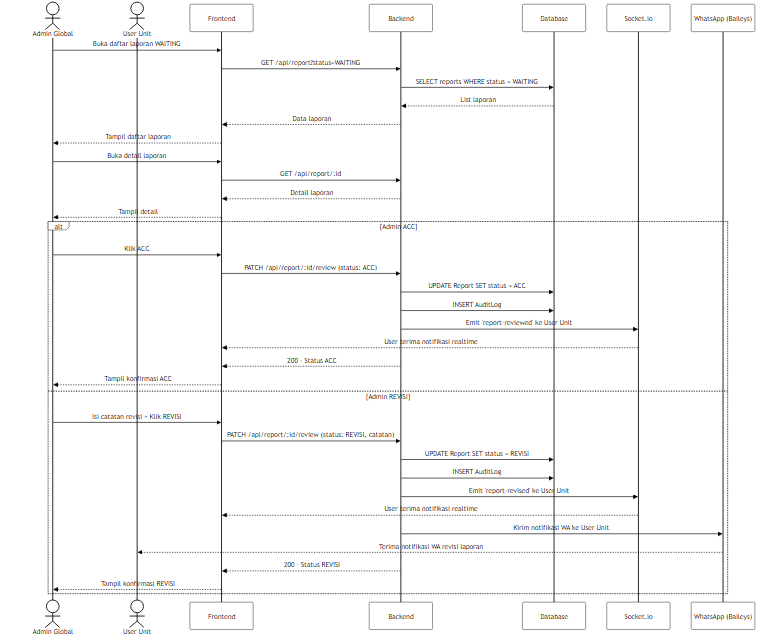
\includegraphics[width=0.95\textwidth]{figure/sequence-admin-review.png}
    \caption{\textit{Sequence Diagram} 4: Admin Review Laporan}
    \label{fig:3.seq-review}
\end{figure}

\textbf{Sequence Diagram 5: Helpdesk REVISION.} \par
Proses \textit{helpdesk} jenis REVISION melibatkan komunikasi antara User Unit, Admin Global, Frontend, Backend, Database, Socket.io, dan layanan WhatsApp. Proses ini dirancang untuk memastikan bahwa perubahan terhadap laporan yang sudah di-\textit{submit} tetap terkontrol dan melalui persetujuan pihak yang berwenang. Alur komunikasi antar komponen dalam proses \textit{helpdesk} REVISION ini dapat dilihat pada Gambar \ref{fig:3.seq-helpdesk} berikut. \par
\begin{figure}[H]
    \centering
    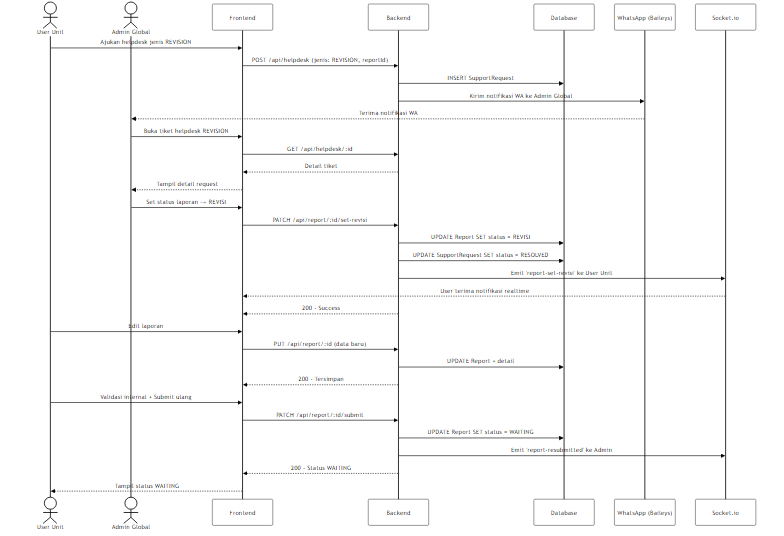
\includegraphics[width=0.95\textwidth]{figure/sequence-helpdesk-revision.png}
    \caption{\textit{Sequence Diagram} 5: Helpdesk REVISION}
    \label{fig:3.seq-helpdesk}
\end{figure}

Berdasarkan \textit{sequence diagram} pada Gambar \ref{fig:3.seq-helpdesk}, User Unit mengajukan \textit{helpdesk} REVISION melalui \texttt{POST /api/helpdesk} dan \textit{backend} menyimpan SupportRequest ke \textit{database} sekaligus mengirimkan notifikasi WhatsApp kepada Admin Global. Admin Global membuka detail tiket melalui \texttt{GET /api/helpdesk/:id} dan apabila menyetujui revisi, mengirimkan \texttt{PATCH /api/report/:id/set-revisi} sehingga \textit{backend} memperbarui status laporan menjadi REVISI, mengubah status SupportRequest menjadi RESOLVED, dan mengirimkan \textit{event} Socket.io agar User Unit menerima notifikasi \textit{real-time}. User Unit kemudian mengedit laporan melalui \texttt{PUT /api/report/:id} dan melakukan validasi internal serta \textit{submit} ulang melalui \texttt{PATCH /api/report/:id/submit}, sehingga \textit{backend} memperbarui status laporan kembali menjadi WAITING dan mengirimkan \textit{event} Socket.io kepada Admin Global bahwa laporan telah di-\textit{submit} ulang. \par


\FloatBarrier
\subsubsection*{d. Entity Relationship Diagram (ERD)}

Sistem ini memiliki sebelas entitas utama yang saling berelasi satu sama lain. Entitas Pengguna merupakan entitas pusat yang berelasi dengan hampir seluruh entitas lain dalam sistem, memiliki atribut peran untuk membedakan tiga jenis pengguna dalam sistem, serta atribut \texttt{percobaan\_login} dan \texttt{terkunci} untuk mendukung mekanisme keamanan akun. Entitas Unit menyimpan data unit kerja dengan atribut \texttt{jenis\_unit} yang membedakan empat jenis unit, yaitu KNA, Penumpang, Barang, dan Keuangan, di mana satu Pengguna berelasi dengan satu Unit melalui hubungan memiliki. Entitas Token Reset berelasi dengan Pengguna melalui hubungan memiliki dan menyimpan atribut \texttt{sudah\_dipakai} serta \texttt{kedaluwarsa\_pada} untuk memastikan token hanya dapat digunakan satu kali dalam batas waktu yang ditentukan. ERD sistem monitoring dan pelaporan kinerja unit PT KAI Divre I Sumatera Utara ini dapat dilihat pada Gambar \ref{fig:3.erd} berikut. \par
\begin{figure}[H]
    \centering
    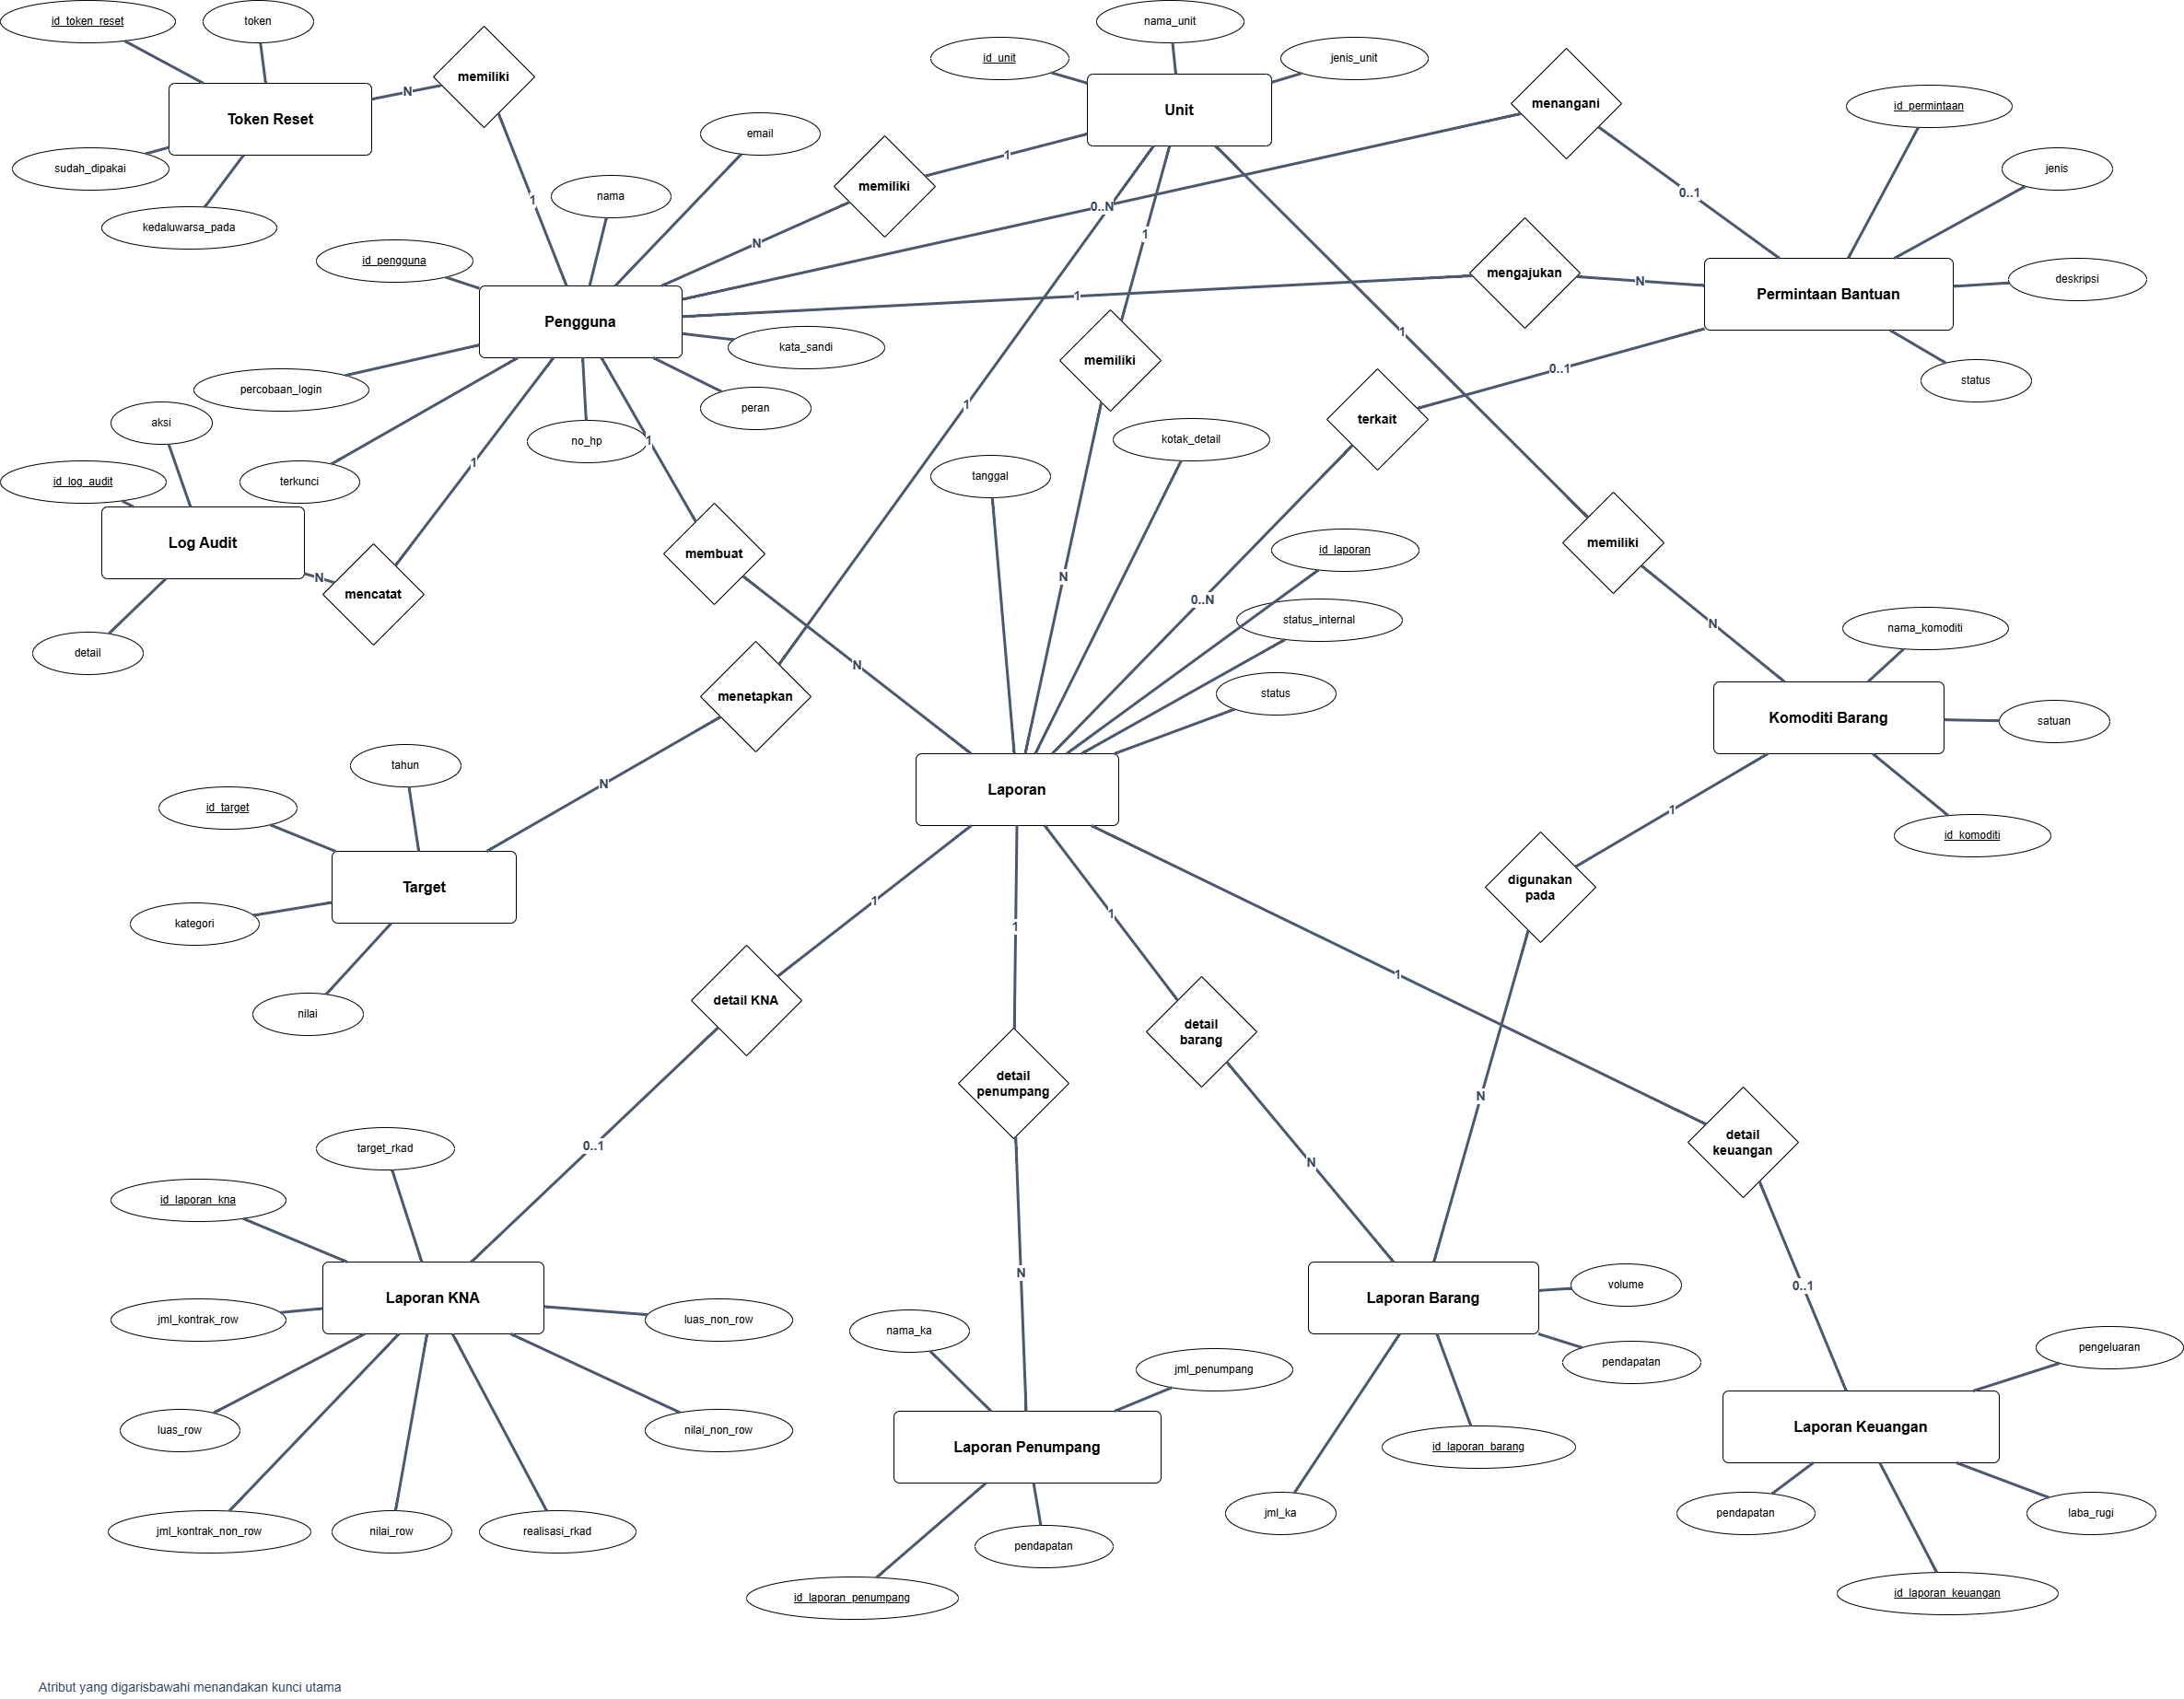
\includegraphics[width=0.95\textwidth]{figure/erdini.drawio (1).png}
    \caption{\textit{Entity Relationship Diagram} Sistem Monitoring dan Pelaporan Kinerja Unit}
    \label{fig:3.erd}
\end{figure}

Berdasarkan ERD pada Gambar \ref{fig:3.erd}, entitas Laporan merupakan inti dari sistem pelaporan yang berelasi dengan Pengguna melalui hubungan membuat, dengan Unit melalui hubungan memiliki, serta memiliki atribut \texttt{status\_internal} dan \texttt{status} untuk merepresentasikan dua tingkat validasi yang berlaku dalam sistem. Laporan berelasi dengan empat entitas detail sesuai jenis unitnya, yaitu Laporan KNA, Laporan Penumpang, Laporan Barang, dan Laporan Keuangan, masing-masing melalui hubungan relasi detail KNA, detail penumpang, detail barang, dan detail keuangan. Entitas Laporan Barang secara khusus berelasi dengan entitas Komoditi Barang melalui hubungan digunakan pada, di mana satu komoditi dapat digunakan pada banyak laporan barang sehingga mendukung pengelolaan komoditi yang bersifat dinamis. Entitas Target berelasi dengan Pengguna melalui hubungan menetapkan dan menyimpan data target kinerja per tahun dan per kategori sebagai acuan perbandingan terhadap data realisasi pada laporan. \par


Entitas Permintaan Bantuan berelasi dengan Pengguna melalui dua hubungan berbeda, yaitu mengajukan untuk pengguna yang mengajukan tiket dan menangani untuk pengguna yang menanganinya, serta memiliki atribut jenis yang membedakan tiga jenis tiket yaitu TOKEN, ISSUE, dan REVISION. Entitas ini juga berelasi dengan Laporan melalui hubungan terkait dengan kardinalitas 0..1 yang menunjukkan bahwa tidak semua permintaan bantuan selalu berkaitan dengan laporan tertentu. Entitas Log Audit berelasi dengan Pengguna melalui hubungan mencatat dan menyimpan seluruh rekam jejak aktivitas penting dalam sistem secara otomatis, mencakup atribut aksi dan detail untuk keperluan penelusuran riwayat. Keseluruhan sebelas entitas ini membentuk struktur basis data yang saling terhubung dan mendukung seluruh alur fungsional sistem secara menyeluruh. \par

\subsubsection*{e. Desain Mid Fidelity}
Desain \textit{mid fidelity} merupakan representasi antarmuka sistem yang lebih detail dibandingkan desain \textit{low fidelity}, dengan penambahan elemen visual seperti warna, font, dan aset grafis final. Rancangan ini disusun sebelum proses implementasi dimulai sebagai panduan bagi pengembang dalam membangun tampilan antarmuka yang sesuai dengan kebutuhan pengguna. Pada penelitian ini, desain \textit{mid fidelity} mencakup seluruh halaman utama yang digunakan oleh ketiga aktor sistem dan disusun menggunakan perangkat Figma.

\textbf{1. Halaman Login Sistem.} \par
Halaman login merupakan halaman pertama yang dihadapi seluruh pengguna saat mengakses sistem dan berfungsi sebagai gerbang autentikasi. Halaman ini memuat formulir login dengan kolom email dan kata sandi, serta menampilkan umpan balik berupa pesan kesalahan dengan informasi sisa percobaan apabila kredensial tidak sesuai, dan pesan akun terkunci beserta tombol Ajukan Helpdesk apabila akun telah dikunci. Rancangan halaman login sistem dapat dilihat pada Gambar \ref{fig:3.lofi-01} berikut.

\begin{figure}[H]
    \centering
    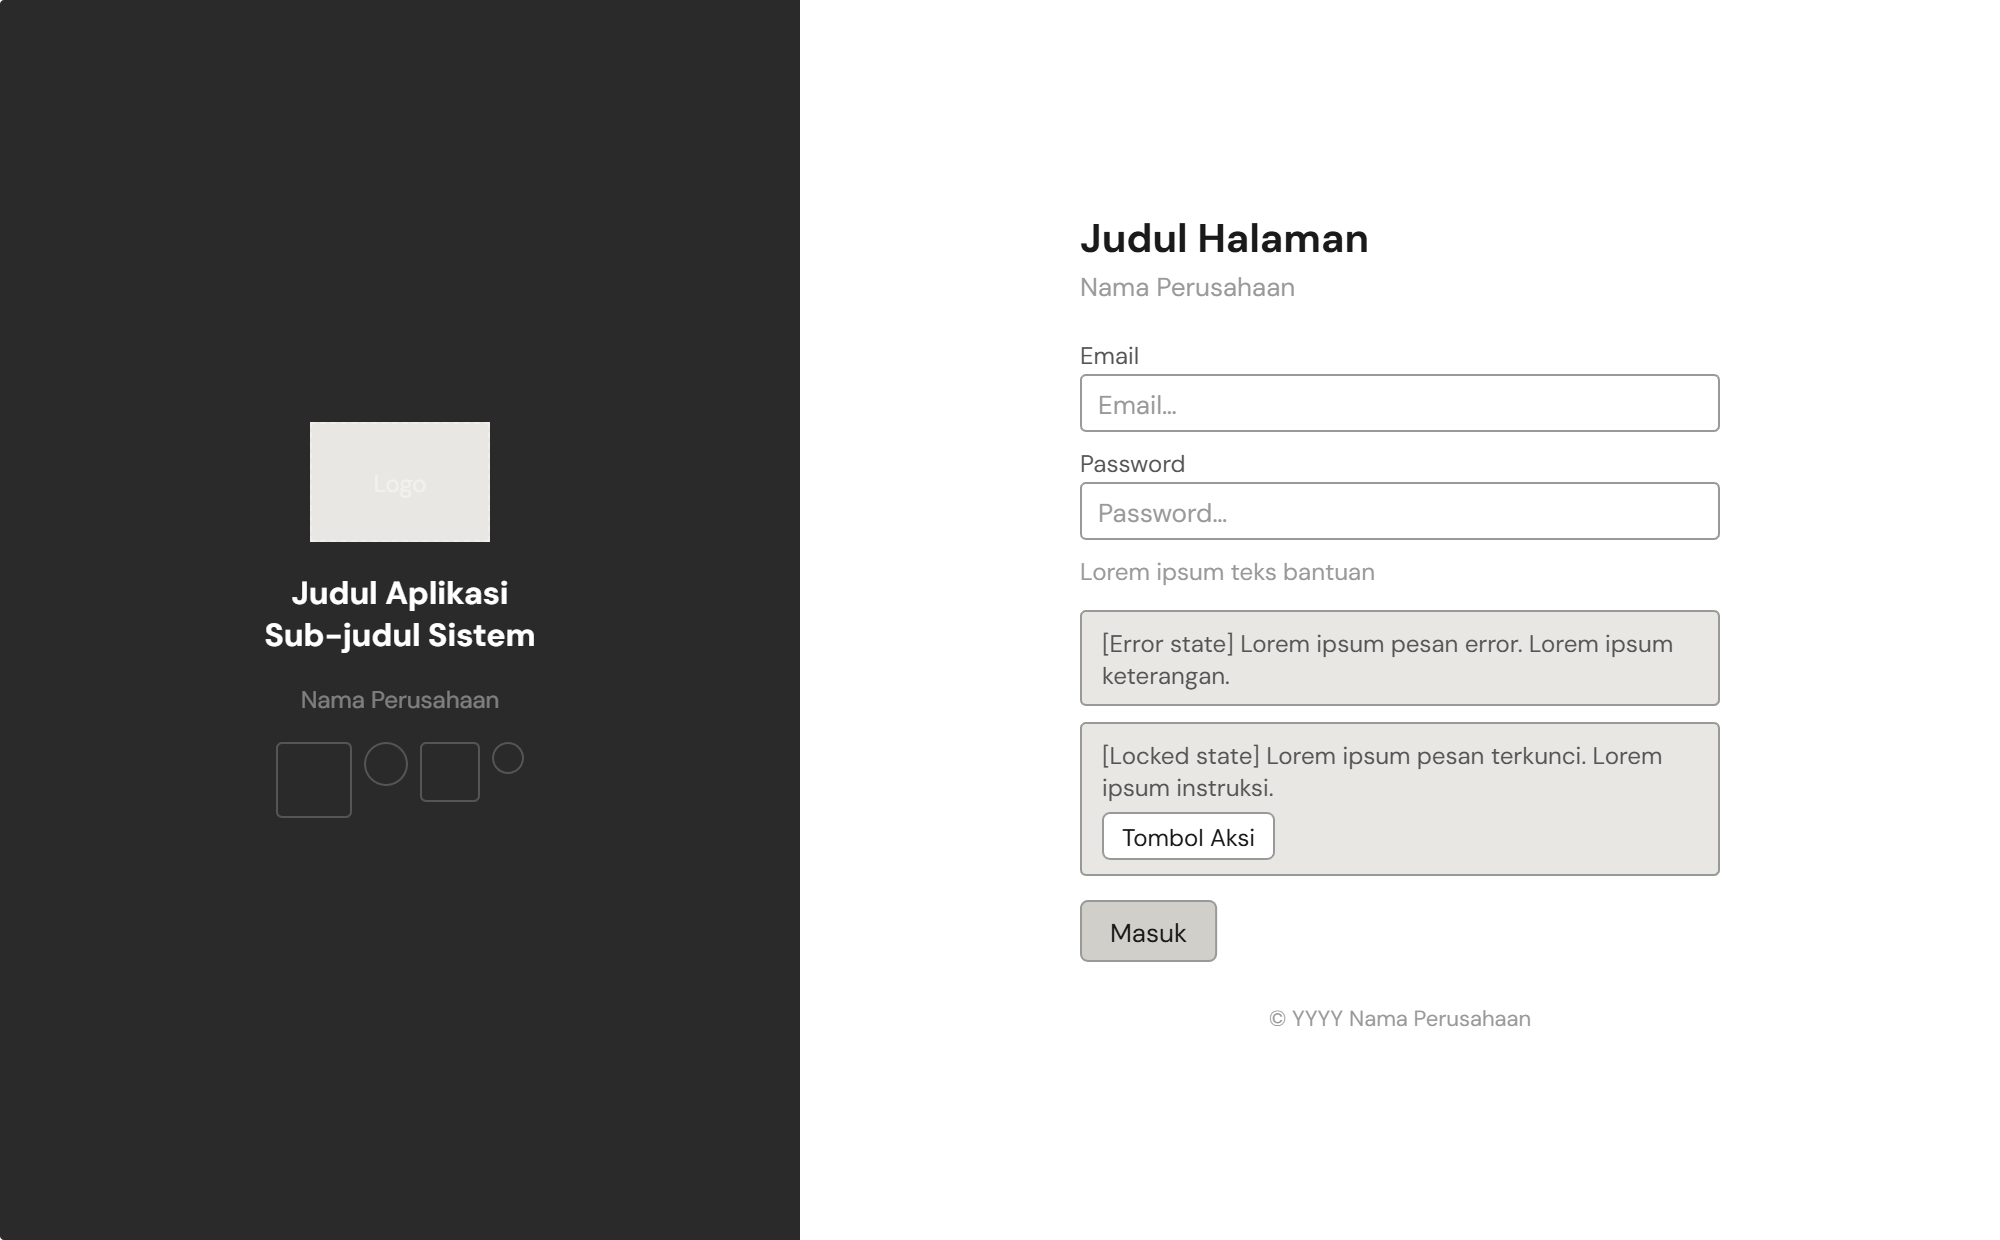
\includegraphics[width=0.85\textwidth]{figure/generated/lowfi-01-login.png}
    \caption{Desain \textit{Mid Fidelity} Halaman Login Sistem}
    \label{fig:3.lofi-01}
\end{figure}

\textbf{2. Halaman Reset Password.} \par
Halaman reset password merupakan halaman yang diakses pengguna setelah menerima token pemulihan yang dikirimkan melalui WhatsApp oleh IT Support. Halaman ini memuat kolom token, kolom kata sandi baru beserta indikator kekuatan kata sandi, dan kolom konfirmasi kata sandi, serta menampilkan pesan kesalahan apabila token tidak valid atau kedaluwarsa. Rancangan halaman reset password dapat dilihat pada Gambar \ref{fig:3.lofi-02} berikut.

\begin{figure}[H]
    \centering
    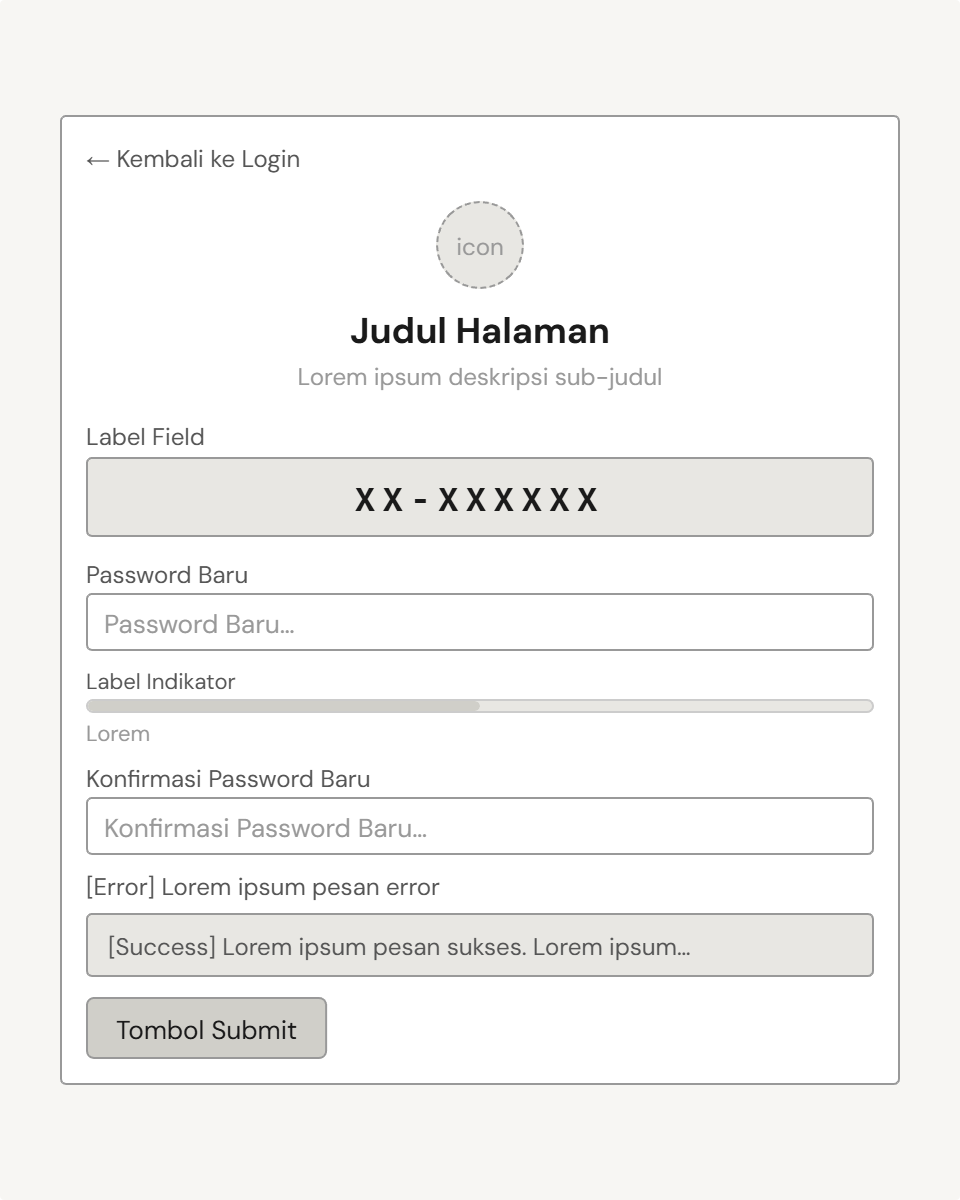
\includegraphics[width=0.85\textwidth]{figure/generated/lowfi-02-reset-password.png}
    \caption{Desain \textit{Mid Fidelity} Halaman Reset Password}
    \label{fig:3.lofi-02}
\end{figure}

\textbf{3. Halaman Dashboard Utama Admin Global.} \par
Rancangan halaman dashboard utama Admin Global ditunjukkan pada Gambar \ref{fig:3.lofi-03}.

\begin{figure}[H]
    \centering
    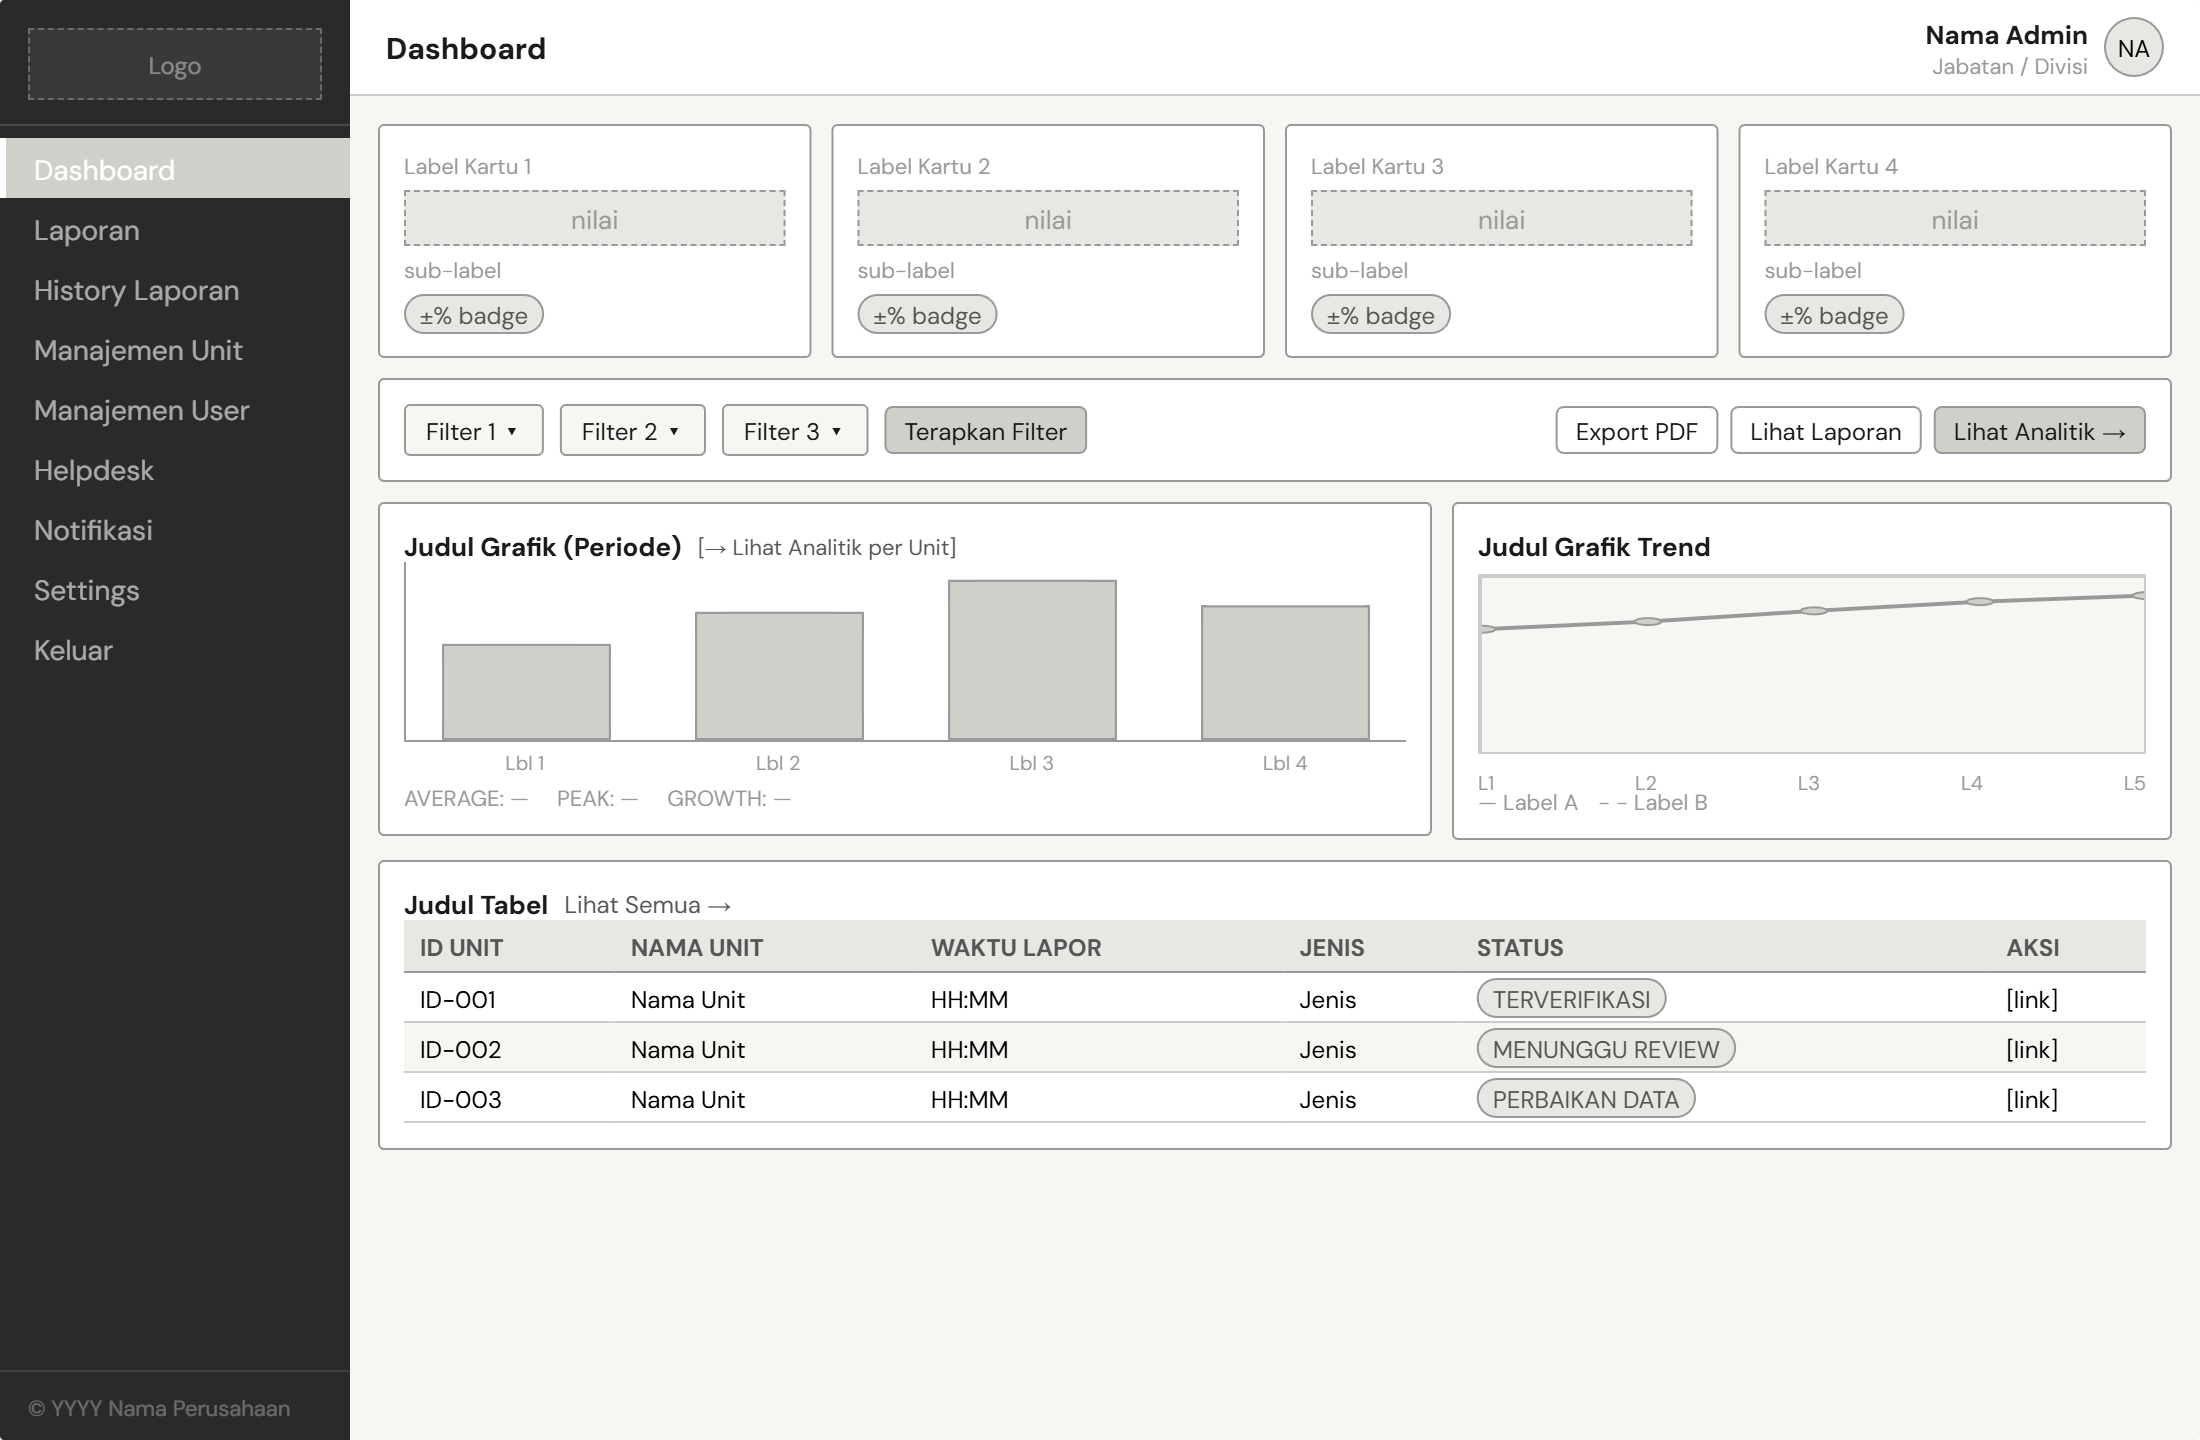
\includegraphics[width=0.85\textwidth]{figure/generated/lowfi-03-dashboard-admin.png}
    \caption{Desain \textit{Mid Fidelity} Halaman Dashboard Utama Admin Global}
    \label{fig:3.lofi-03}
\end{figure}

Berdasarkan Gambar \ref{fig:3.lofi-03}, halaman ini merupakan halaman pertama yang ditampilkan kepada Admin Global setelah masuk dan berfungsi sebagai pusat pemantauan kinerja seluruh unit secara menyeluruh. Halaman ini memuat kartu ringkasan kinerja per unit, grafik tren mingguan dan tahunan, filter data, serta tabel status pelaporan unit terakhir beserta tombol aksi untuk tindak lanjut langsung. \par

\textbf{4. Halaman History Laporan (Admin Global).} \par
Halaman history laporan menyediakan rekam jejak seluruh laporan yang pernah diproses dalam sistem dan dapat diakses oleh Admin Global untuk keperluan penelusuran dan evaluasi data historis. Halaman ini memuat filter berdasarkan unit, bulan, tahun, dan status, serta tabel yang menampilkan seluruh laporan lengkap dengan informasi tanggal, unit, jenis, pengaju, status, reviewer, dan tombol aksi. Rancangan halaman history laporan Admin Global dapat dilihat pada Gambar \ref{fig:3.lofi-19a} berikut.

\begin{figure}[H]
    \centering
    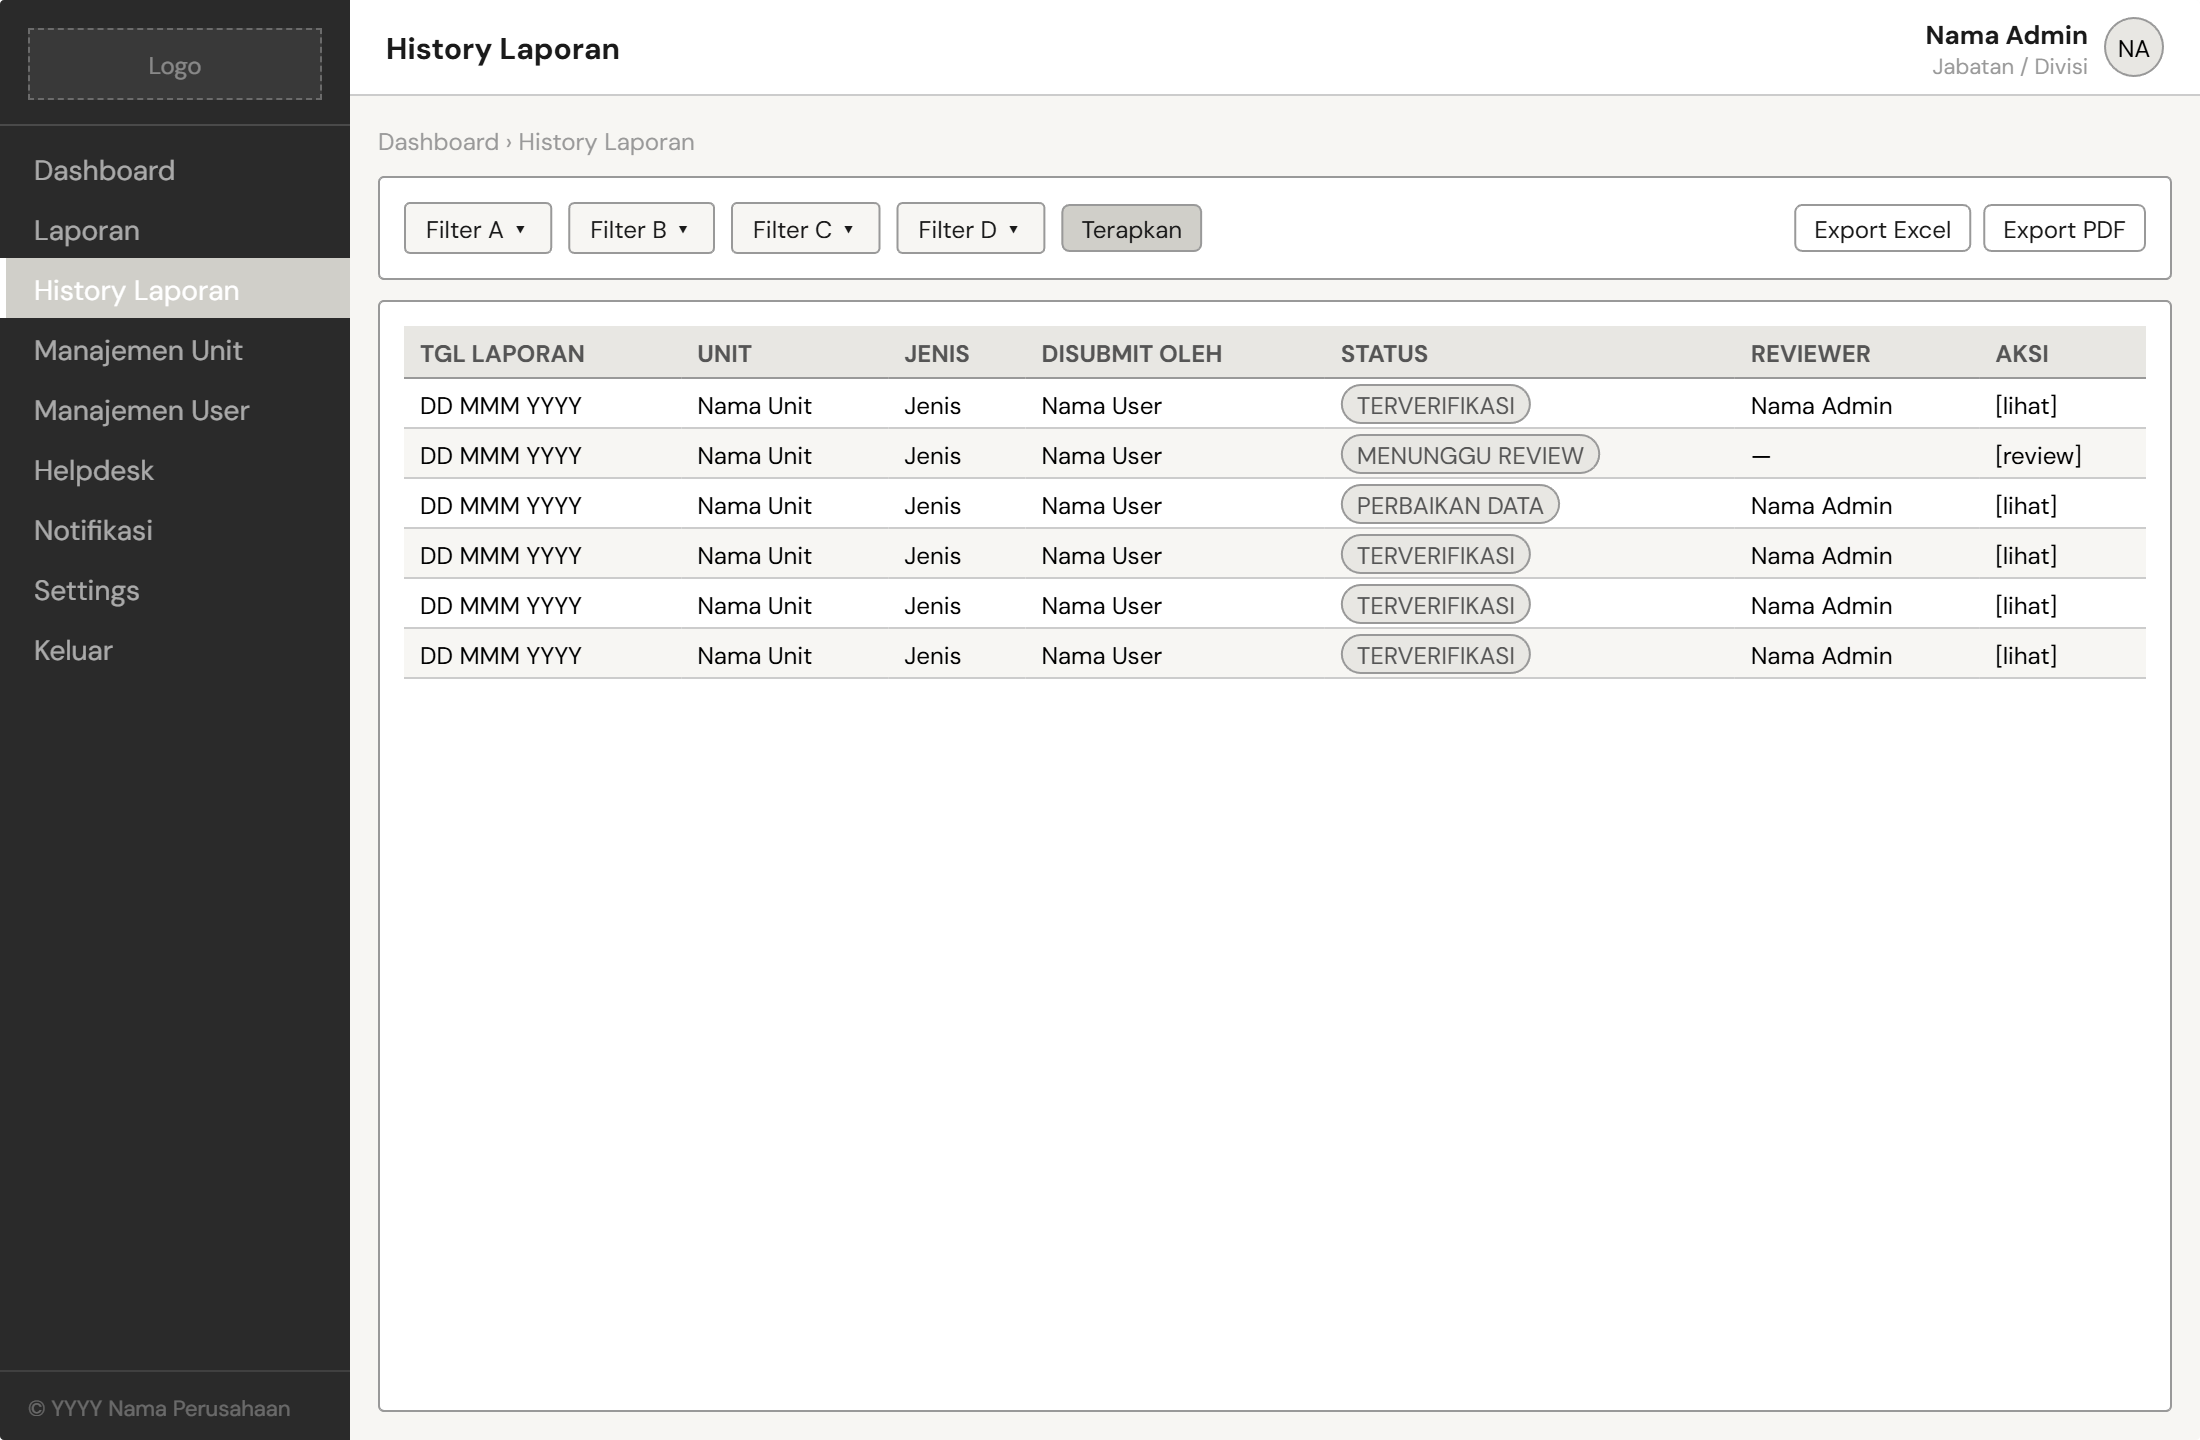
\includegraphics[width=0.85\textwidth]{figure/generated/lowfi-19a-history-laporan-admin.png}
    \caption{Desain \textit{Mid Fidelity} Halaman History Laporan Admin Global}
    \label{fig:3.lofi-19a}
\end{figure}

\textbf{5. Halaman Review Laporan.} \par
\begin{figure}[H]
    \centering
    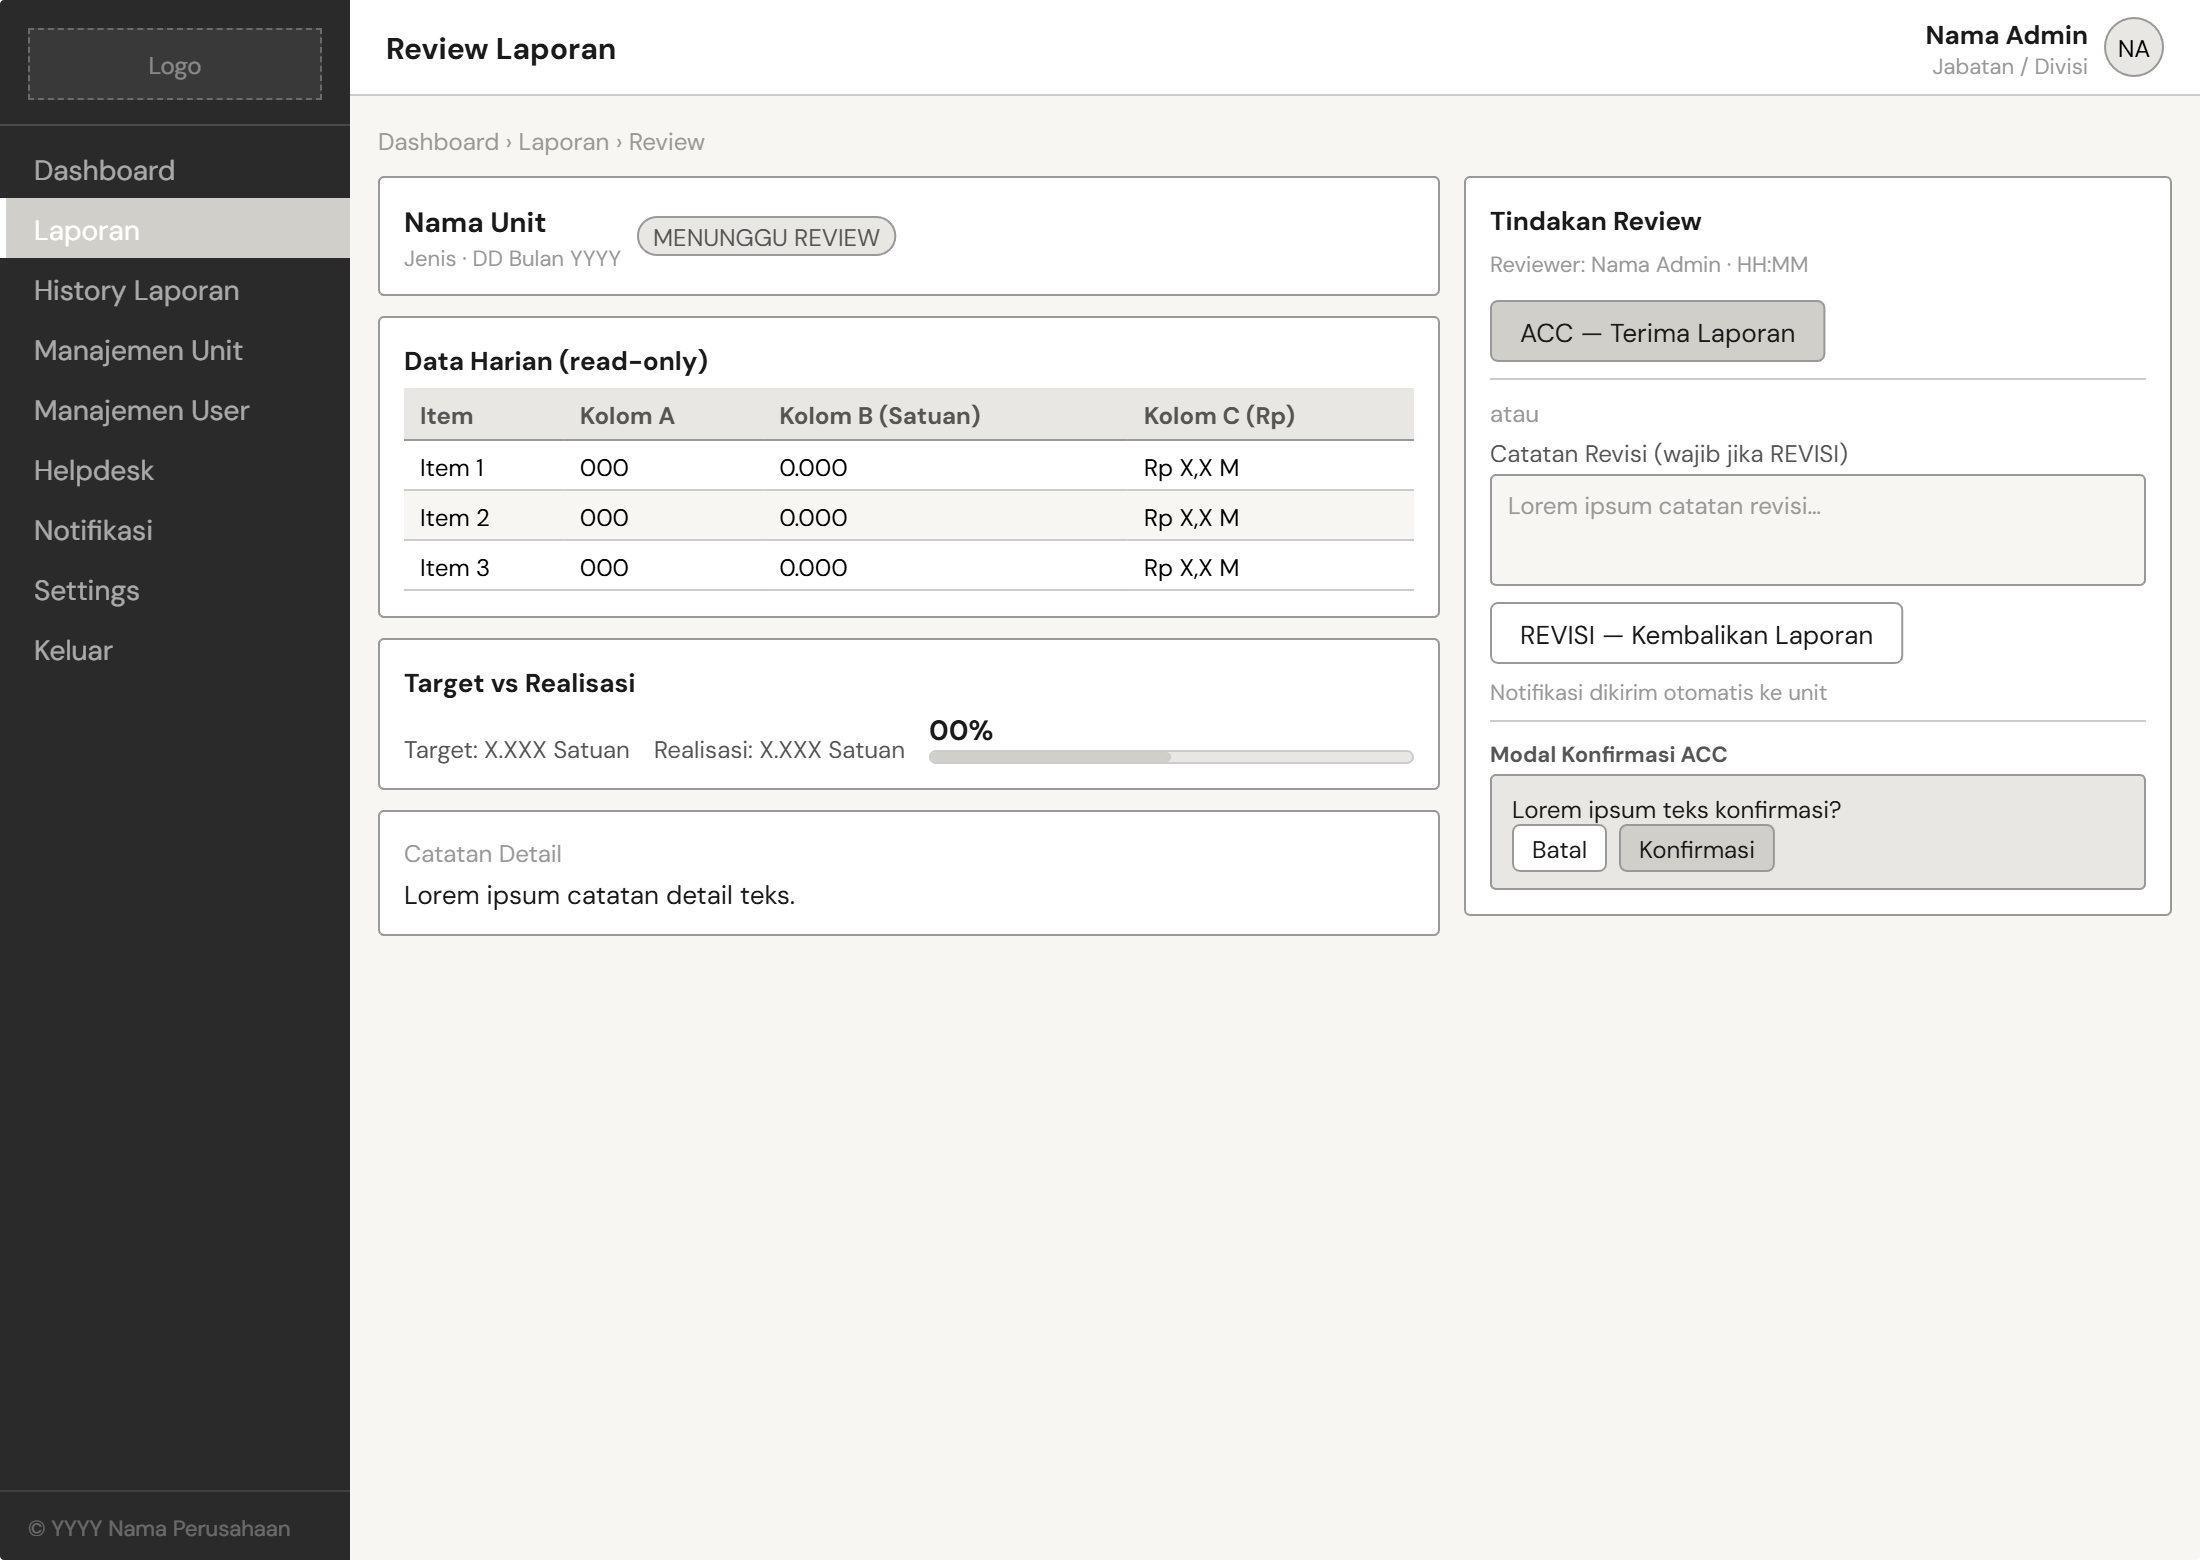
\includegraphics[width=0.85\textwidth]{figure/generated/lowfi-09-review-laporan.png}
    \caption{Desain \textit{Mid Fidelity} Halaman Review Laporan}
    \label{fig:3.lofi-09}
\end{figure}
Rancangan halaman review laporan dapat dilihat pada Gambar \ref{fig:3.lofi-09} diatas. Halaman review laporan merupakan halaman yang digunakan Admin Global untuk meninjau isi laporan yang telah di-\textit{submit} dan memberikan keputusan berupa ACC atau REVISI. Halaman ini menampilkan detail isi laporan dalam mode \textit{read-only} di sisi kiri, serta panel tindakan review di sisi kanan yang memuat tombol ACC, kolom catatan revisi, dan tombol REVISI disertai jendela konfirmasi sebelum keputusan disimpan.

\textbf{6. Halaman Analitik \& Grafik.} \par
Rancangan halaman analitik dan grafik ditunjukkan pada Gambar \ref{fig:3.lofi-13}.

\begin{figure}[H]
    \centering
    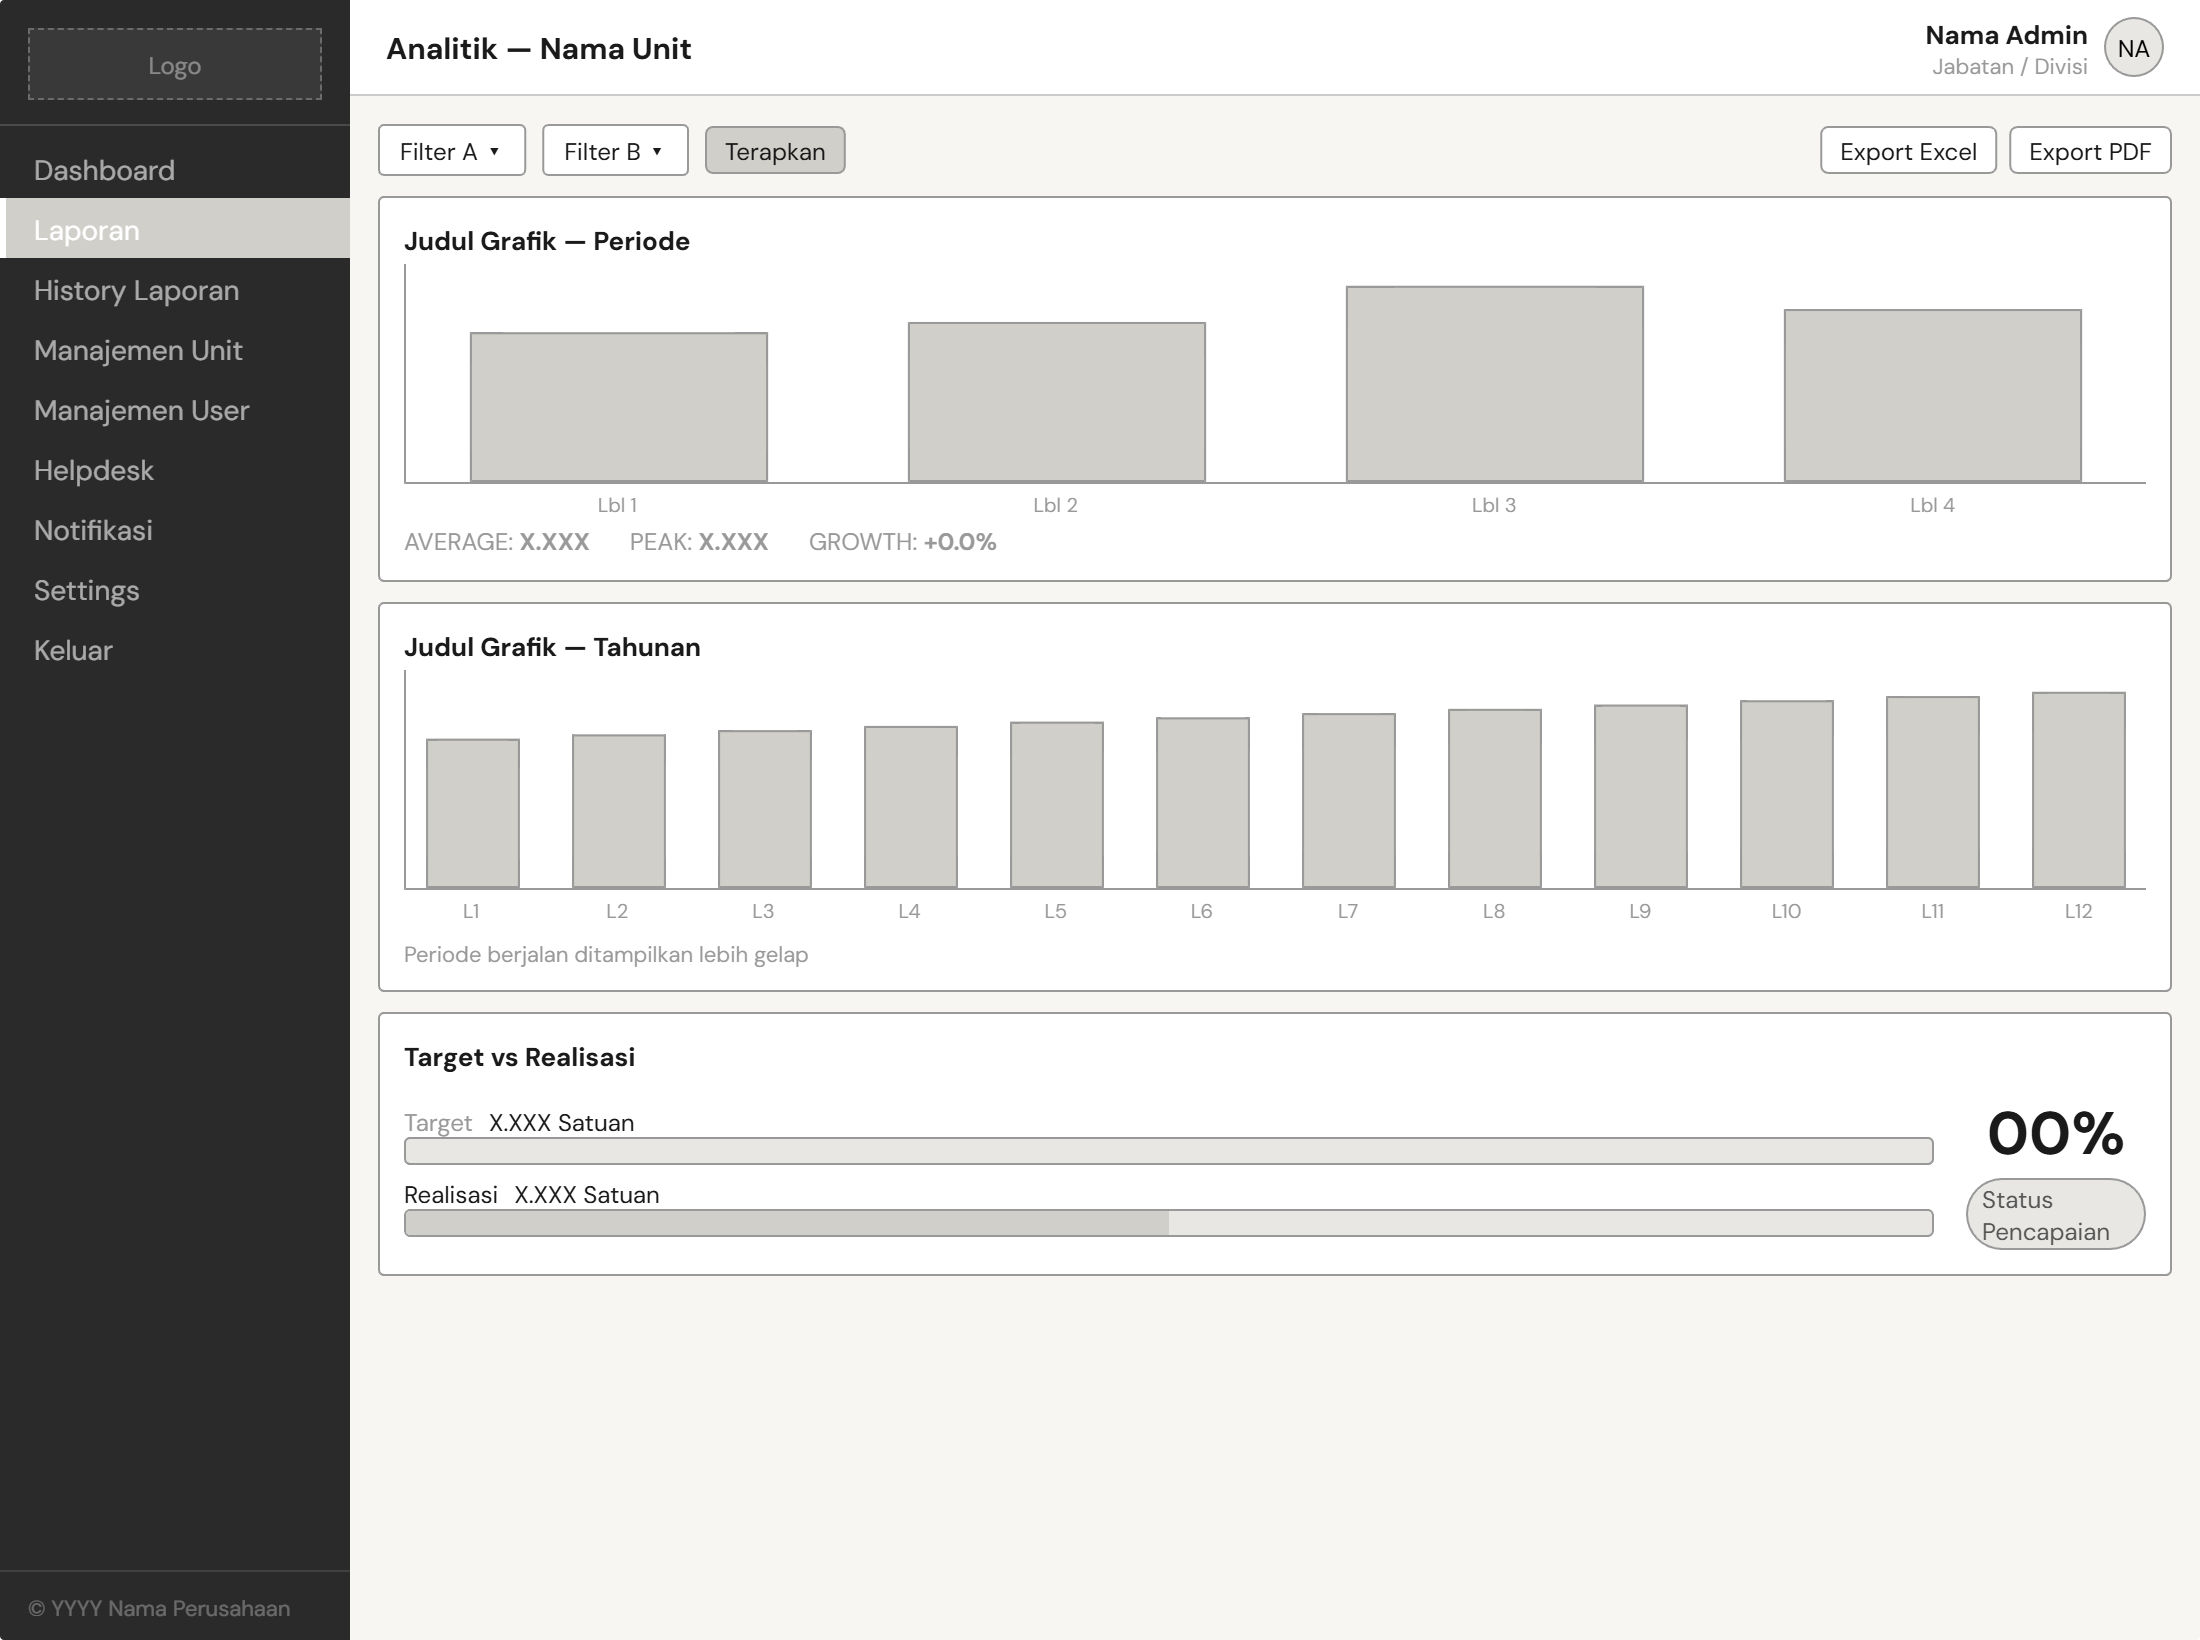
\includegraphics[width=0.85\textwidth]{figure/generated/lowfi-13-analitik-grafik.png}
    \caption{Desain \textit{Mid Fidelity} Halaman Analitik \& Grafik}
    \label{fig:3.lofi-13}
\end{figure}

Berdasarkan Gambar \ref{fig:3.lofi-13}, halaman analitik merupakan halaman yang menyajikan visualisasi data kinerja suatu unit secara lebih mendalam dan dapat diakses Admin Global melalui tombol Lihat Analitik pada \textit{dashboard}. Halaman ini menampilkan grafik batang tren volume mingguan dan bulanan, serta bagian Target vs Realisasi yang memperlihatkan persentase pencapaian unit terhadap target yang telah ditetapkan. \par

\textbf{7. Halaman Manajemen Unit.} \par
Halaman manajemen unit merupakan halaman yang digunakan Admin Global untuk mengelola data seluruh unit kerja yang terdaftar dalam sistem, mencakup penambahan dan perubahan data unit. Halaman ini memuat tabel daftar unit beserta statusnya dan modal Tambah/Edit Unit yang berisi kolom nama unit, penanggung jawab, jenis laporan, dan status. Rancangan halaman manajemen unit dapat dilihat pada Gambar \ref{fig:3.lofi-18} berikut.

\begin{figure}[H]
    \centering
    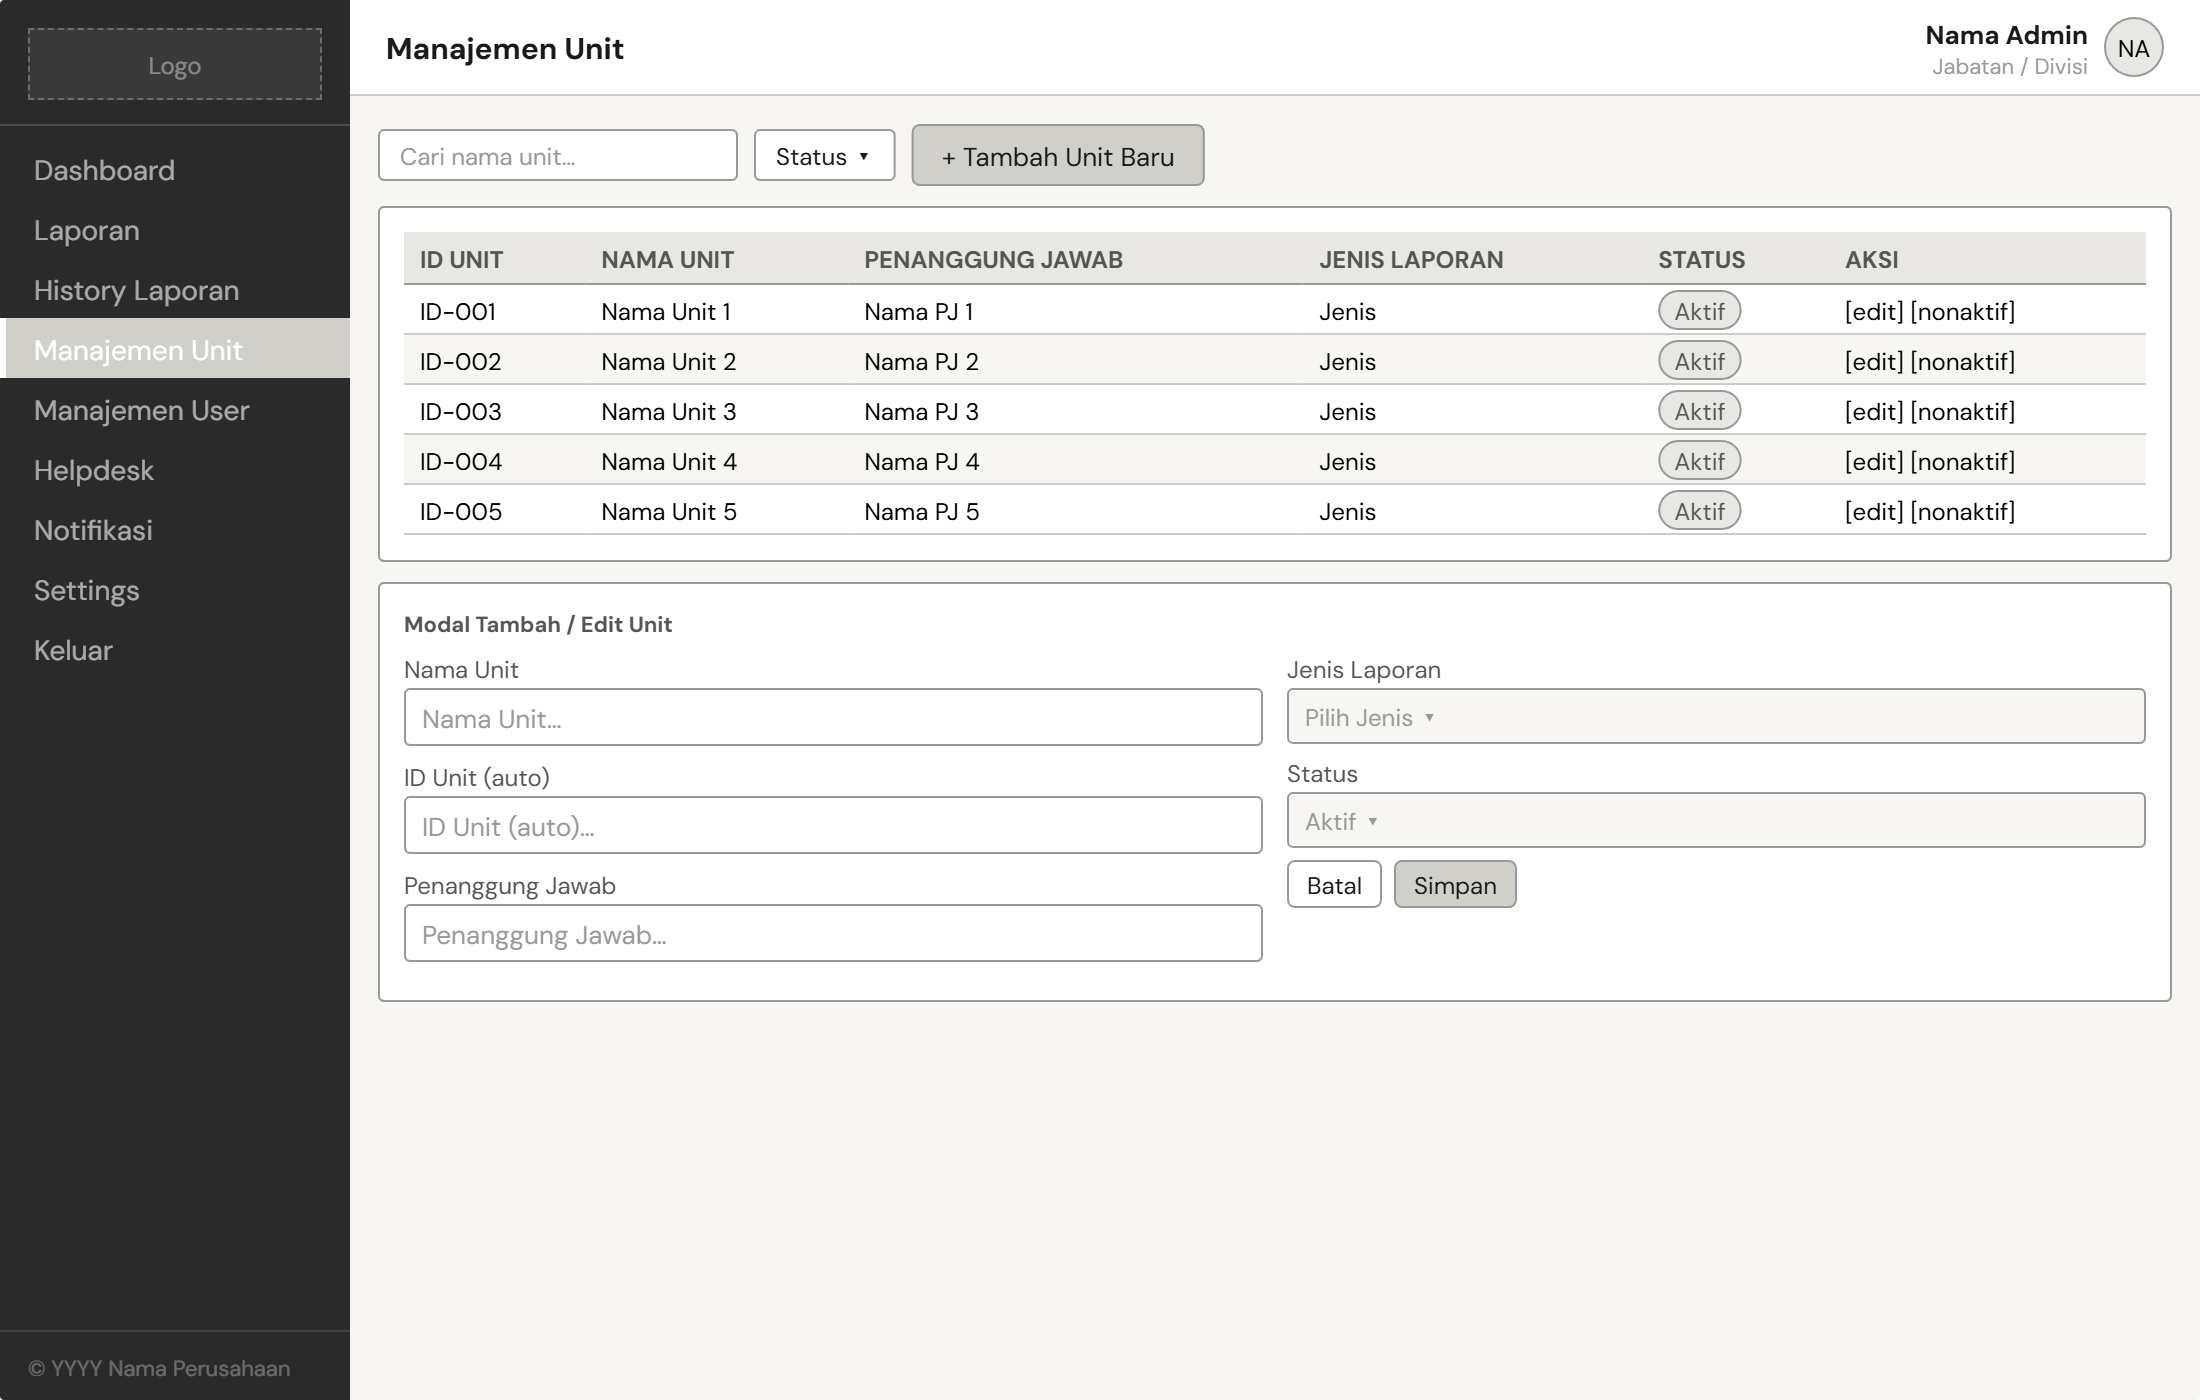
\includegraphics[width=0.85\textwidth]{figure/generated/lowfi-18-manajemen-unit.png}
    \caption{Desain \textit{Mid Fidelity} Halaman Manajemen Unit}
    \label{fig:3.lofi-18}
\end{figure}

\textbf{8. Halaman Manajemen User.} \par
Halaman manajemen user merupakan halaman yang digunakan Admin Global untuk mengelola seluruh akun pengguna yang terdaftar, termasuk pembuatan akun baru, pengeditan data, dan pemantauan status akun. Halaman ini memuat tabel daftar pengguna beserta kondisi akunnya dan modal Tambah/Edit User yang berisi kolom nama, email, nomor WhatsApp, peran, unit, serta kata sandi yang dibangkitkan otomatis oleh sistem. Rancangan halaman manajemen user dapat dilihat pada Gambar \ref{fig:3.lofi-14} berikut.

\begin{figure}[H]
    \centering
    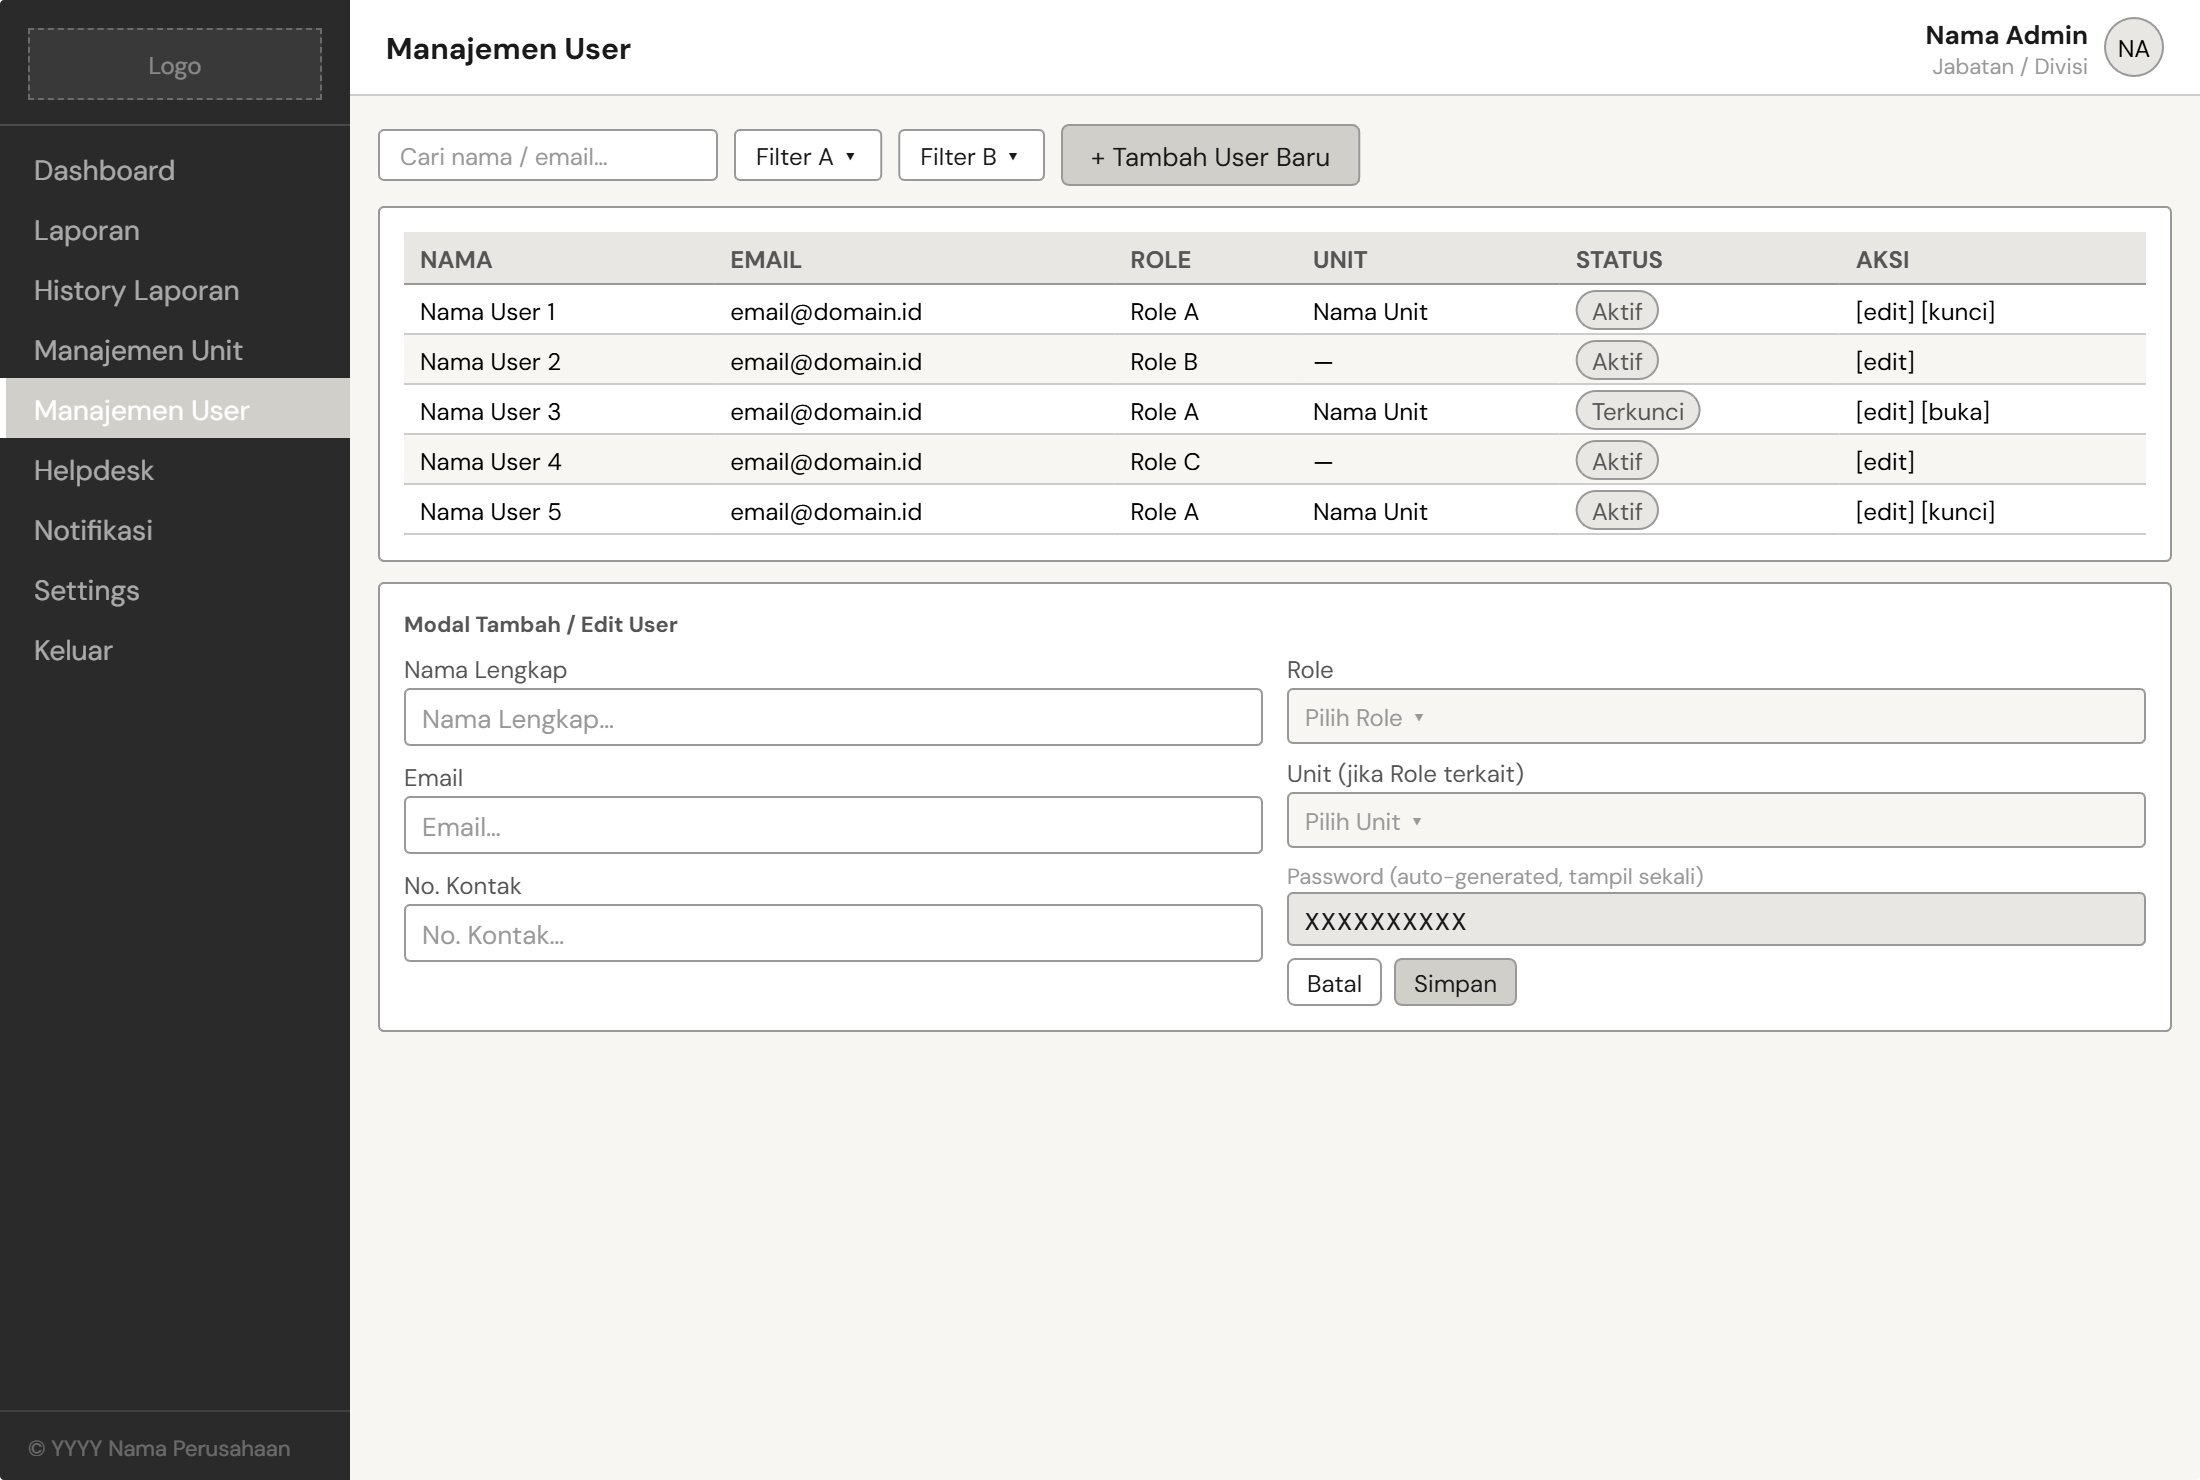
\includegraphics[width=0.85\textwidth]{figure/generated/lowfi-14-manajemen-user.png}
    \caption{Desain \textit{Mid Fidelity} Halaman Manajemen User}
    \label{fig:3.lofi-14}
\end{figure}

\textbf{9. Halaman Manajemen Notifikasi.} \par
Rancangan halaman manajemen notifikasi ditunjukkan pada Gambar \ref{fig:3.lofi-16}.

\begin{figure}[H]
    \centering
    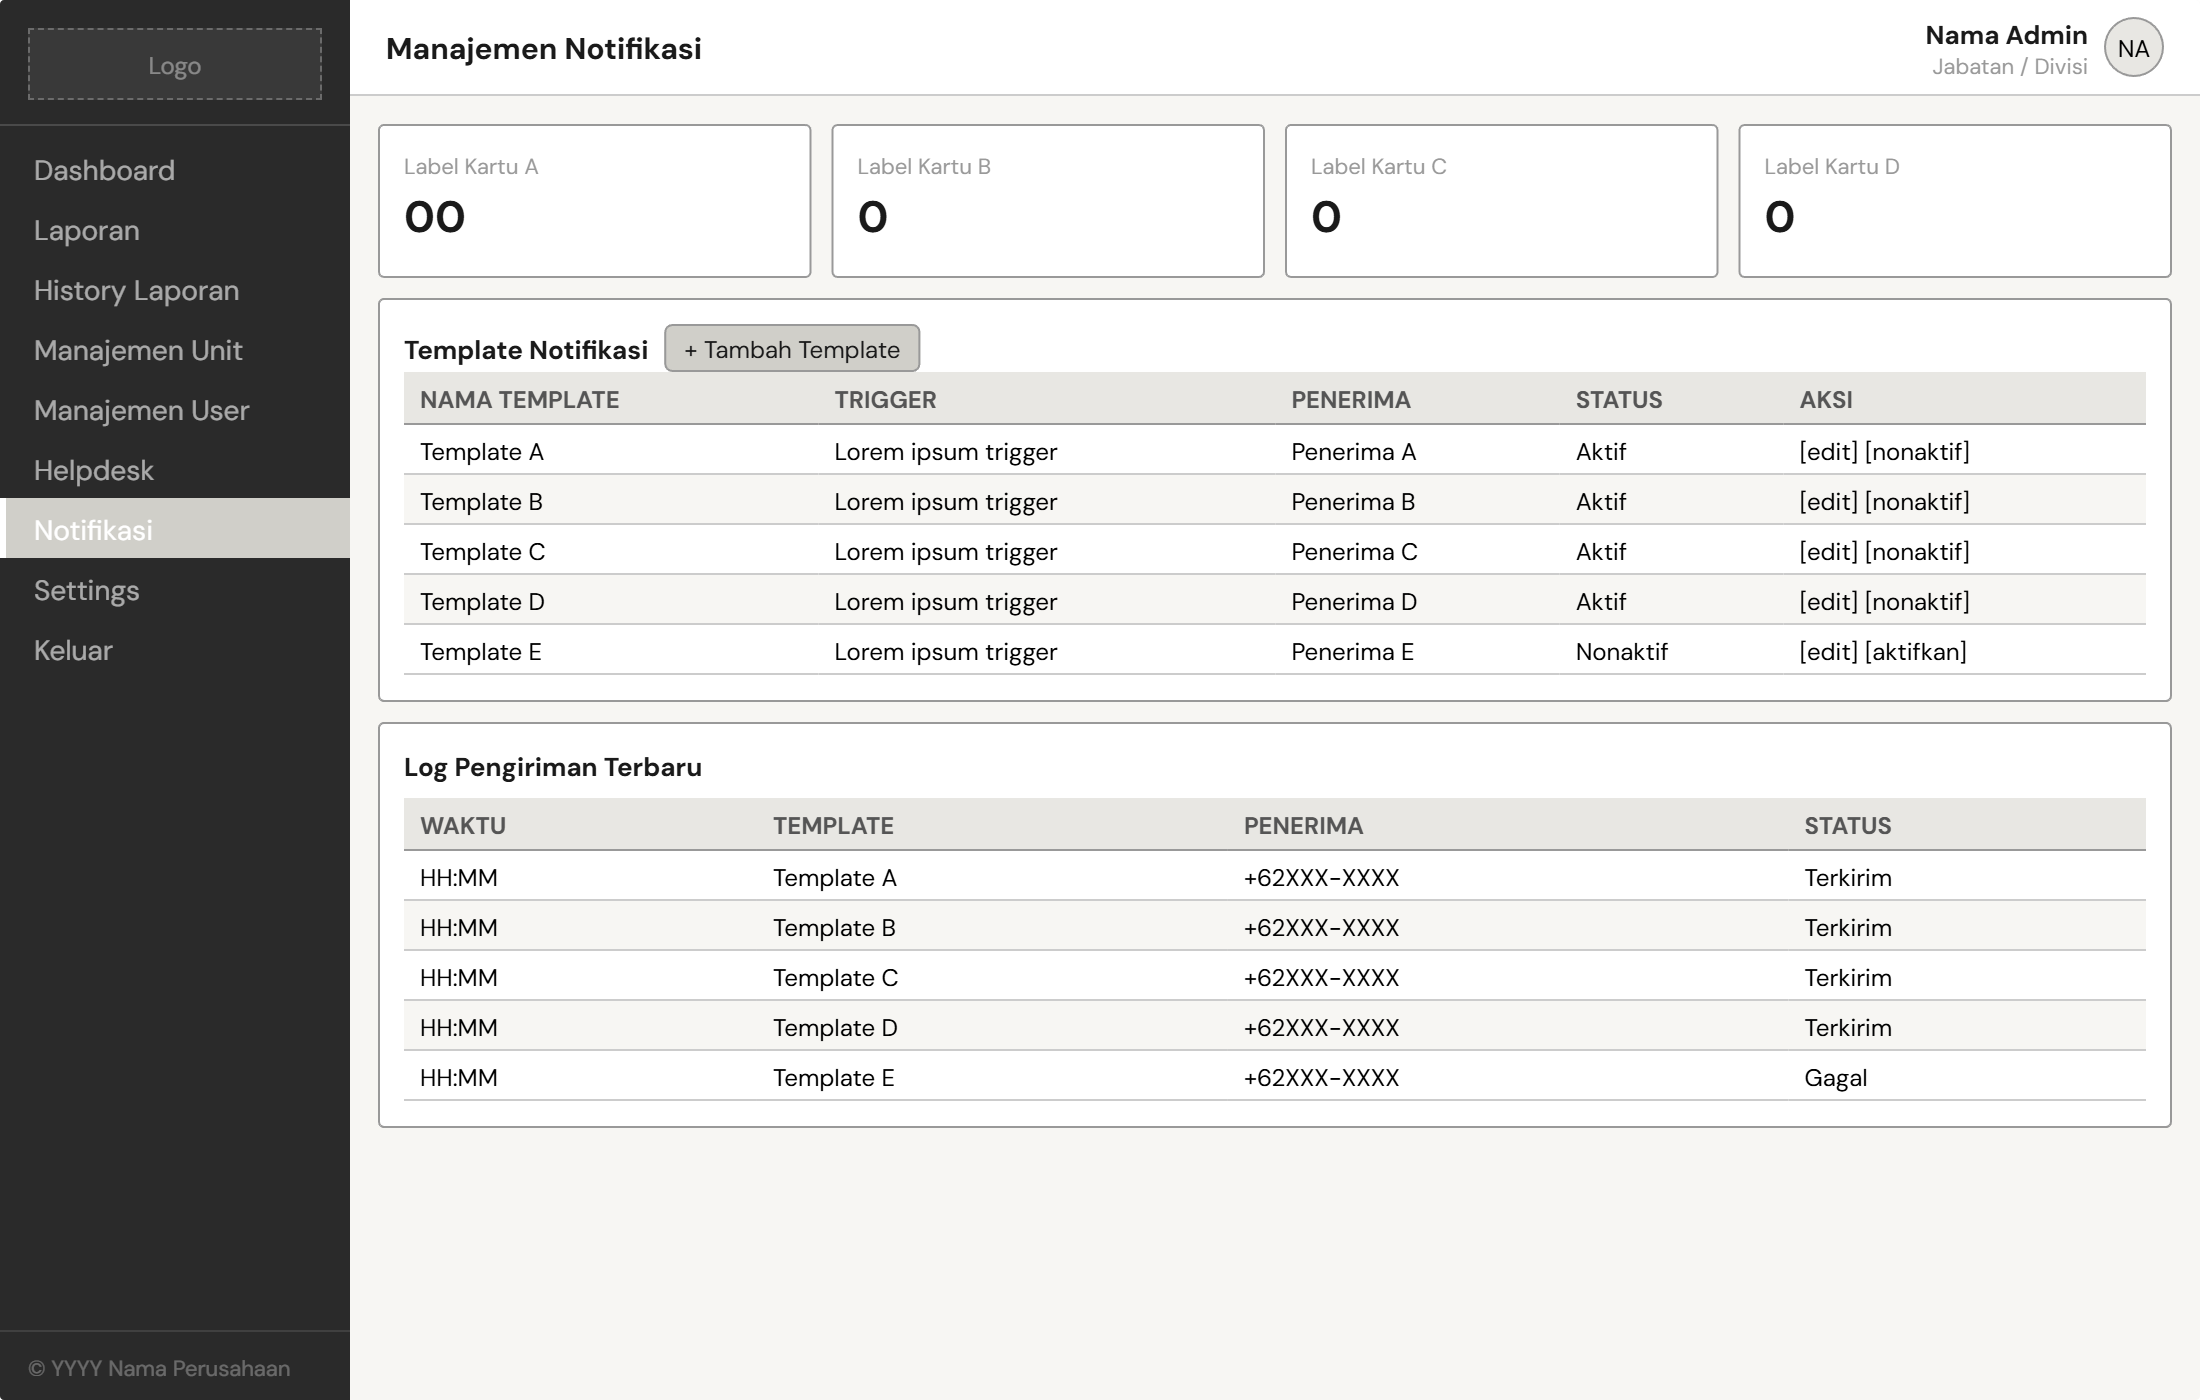
\includegraphics[width=0.85\textwidth]{figure/generated/lowfi-16-manajemen-notifikasi.png}
    \caption{Desain \textit{Mid Fidelity} Halaman Manajemen Notifikasi}
    \label{fig:3.lofi-16}
\end{figure}

Berdasarkan Gambar \ref{fig:3.lofi-16}, halaman manajemen notifikasi merupakan halaman yang digunakan Admin Global untuk memantau dan mengelola seluruh aktivitas pengiriman notifikasi WhatsApp yang berjalan di dalam sistem. Halaman ini memuat kartu ringkasan status pengiriman notifikasi, tabel template notifikasi WhatsApp yang aktif, serta tabel log pengiriman terbaru yang mencatat riwayat notifikasi secara kronologis. \par

\textbf{10. Halaman Settings.} \par
Halaman settings merupakan halaman yang menyediakan pengaturan preferensi tampilan sistem dan dapat diakses oleh Admin Global, User Unit, dan IT Support melalui menu navigasi. Halaman ini memuat pengaturan bahasa antarmuka dan pilihan mode tampilan antara Terang dan Gelap, dilengkapi tombol Simpan dan Reset ke Default. Rancangan halaman settings dapat dilihat pada Gambar \ref{fig:3.lofi-17} berikut.

\begin{figure}[H]
    \centering
    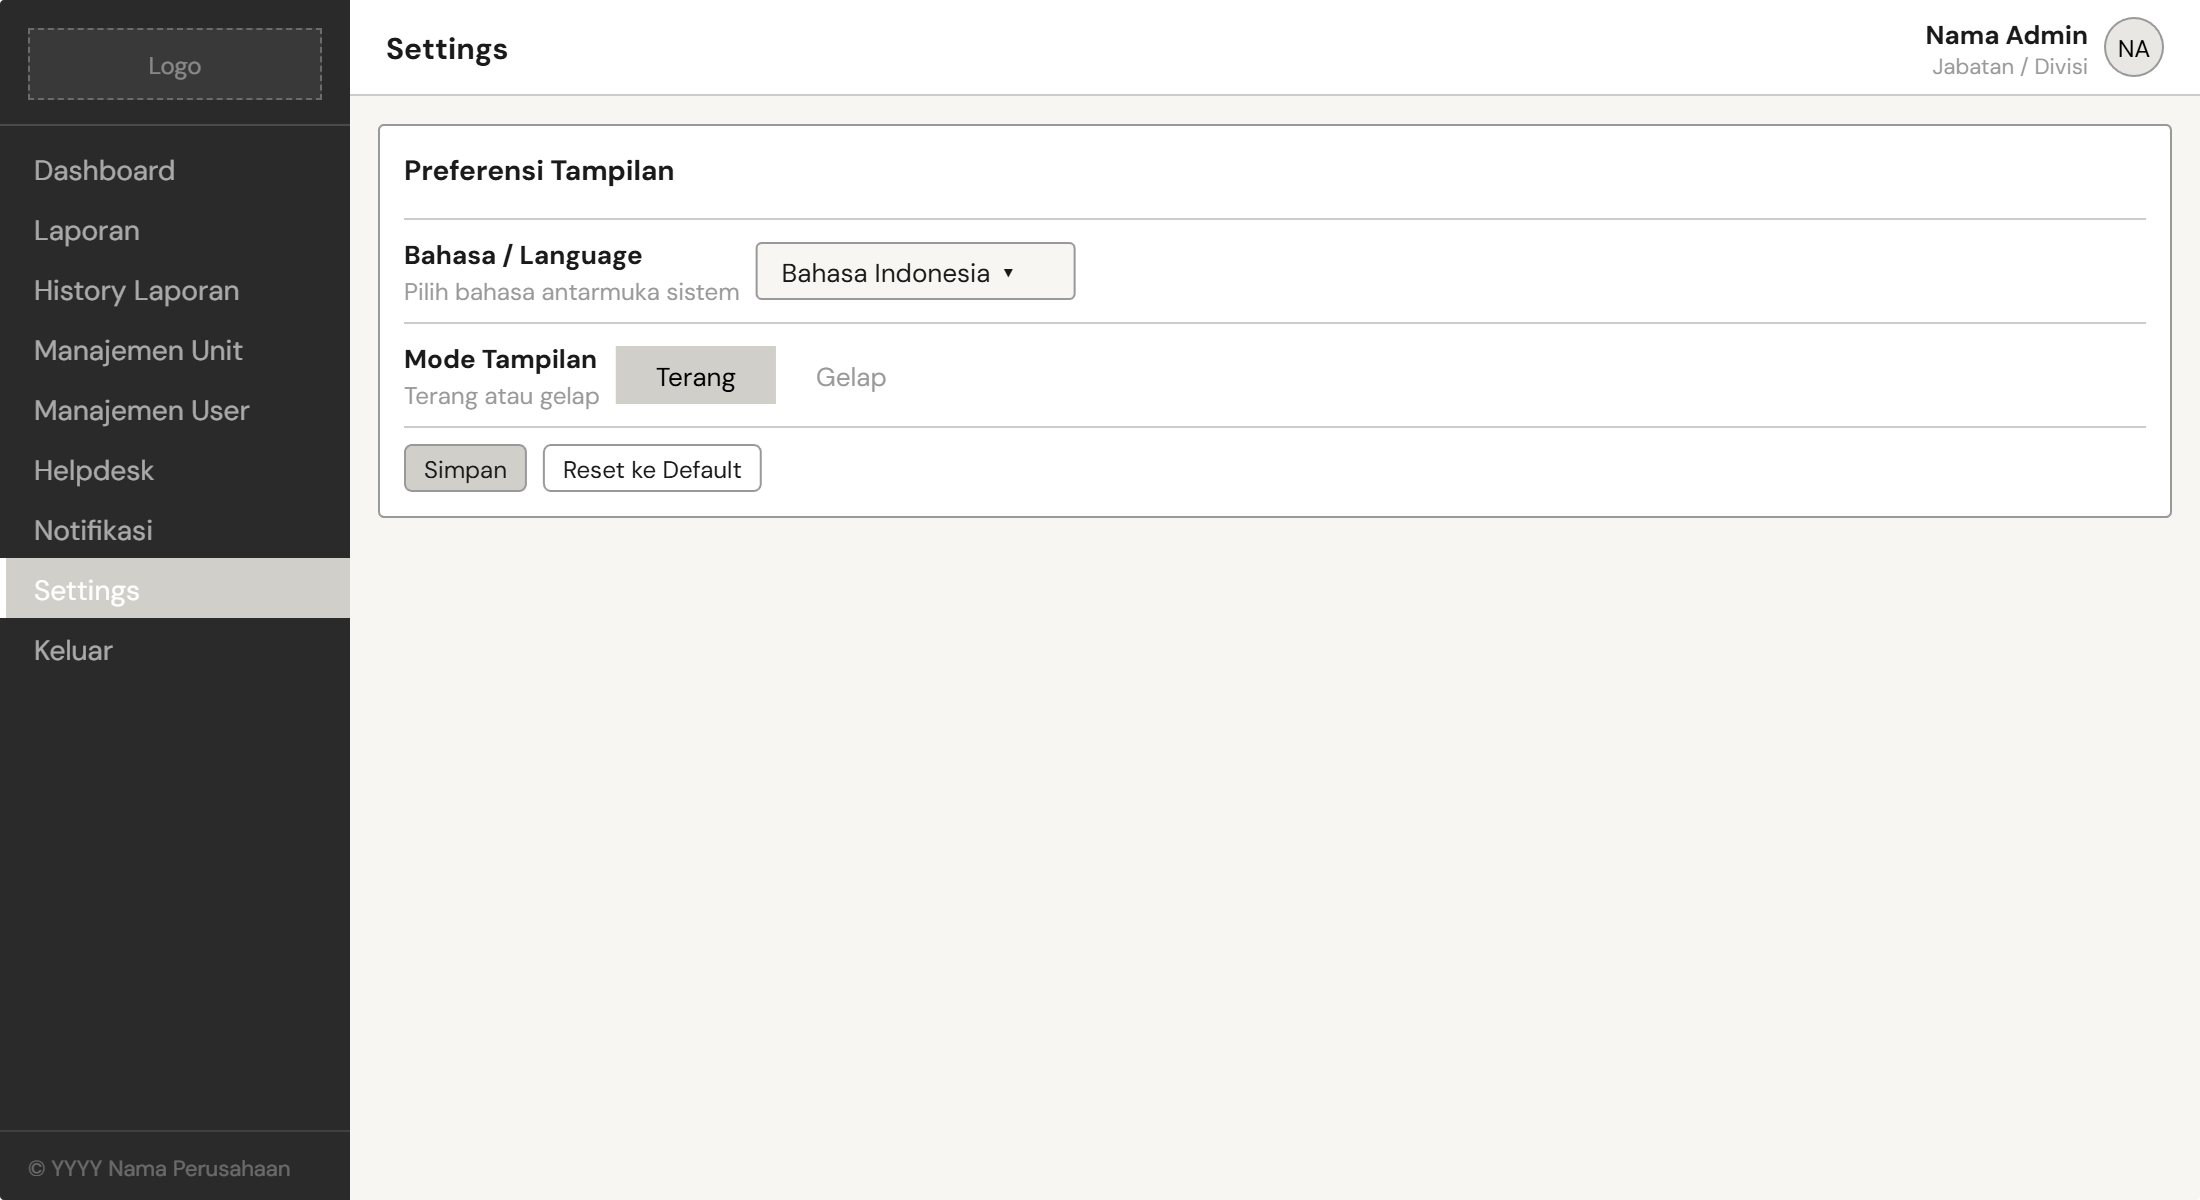
\includegraphics[width=0.85\textwidth]{figure/generated/lowfi-17-settings.png}
    \caption{Desain \textit{Mid Fidelity} Halaman Settings}
    \label{fig:3.lofi-17}
\end{figure}

\textbf{11. Halaman Dashboard User Unit.} \par
Halaman dashboard User Unit merupakan halaman utama yang ditampilkan kepada User Unit setelah masuk dan dirancang untuk memberikan gambaran cepat mengenai status pelaporan unitnya. Halaman ini memuat peringatan otomatis apabila laporan belum di-\textit{submit}, kartu ringkasan status laporan, grafik tren mingguan, serta tabel \textit{history} laporan terbaru. Rancangan halaman dashboard User Unit dapat dilihat pada Gambar \ref{fig:3.lofi-04} berikut.

\begin{figure}[H]
    \centering
    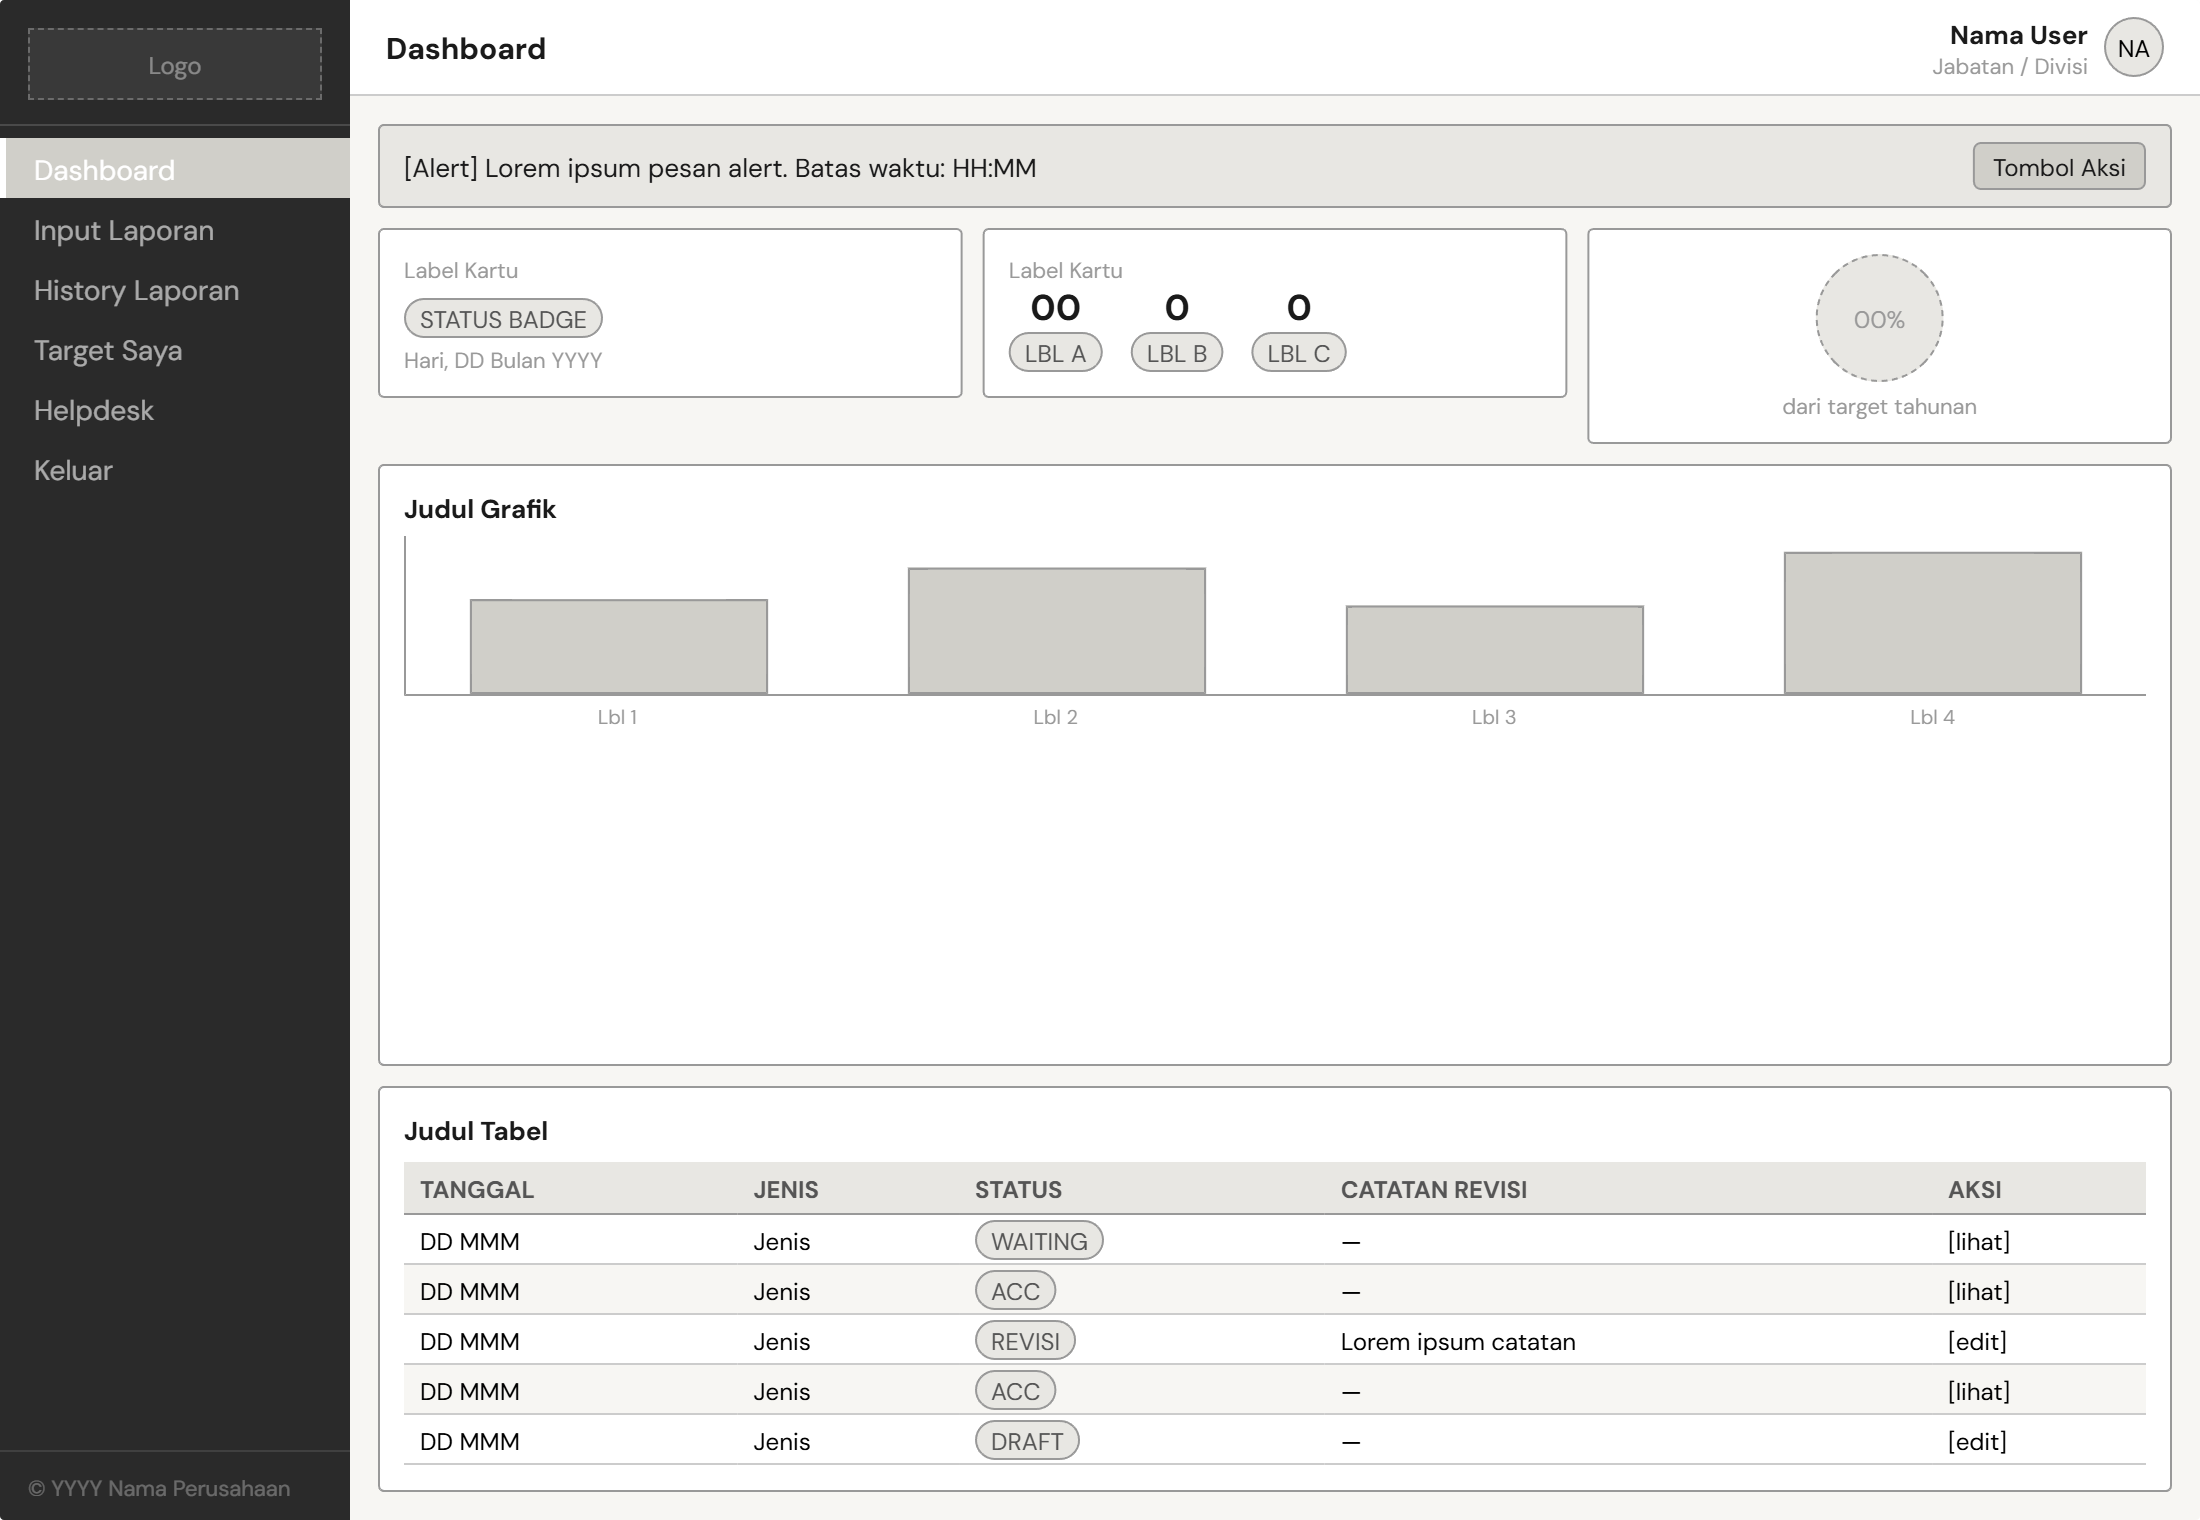
\includegraphics[width=0.85\textwidth]{figure/generated/lowfi-04-dashboard-user-unit.png}
    \caption{Desain \textit{Mid Fidelity} Halaman Dashboard User Unit}
    \label{fig:3.lofi-04}
\end{figure}

\textbf{12. Halaman Input Laporan Harian Unit Angkutan Barang.} \par
\begin{figure}[H]
    \centering
    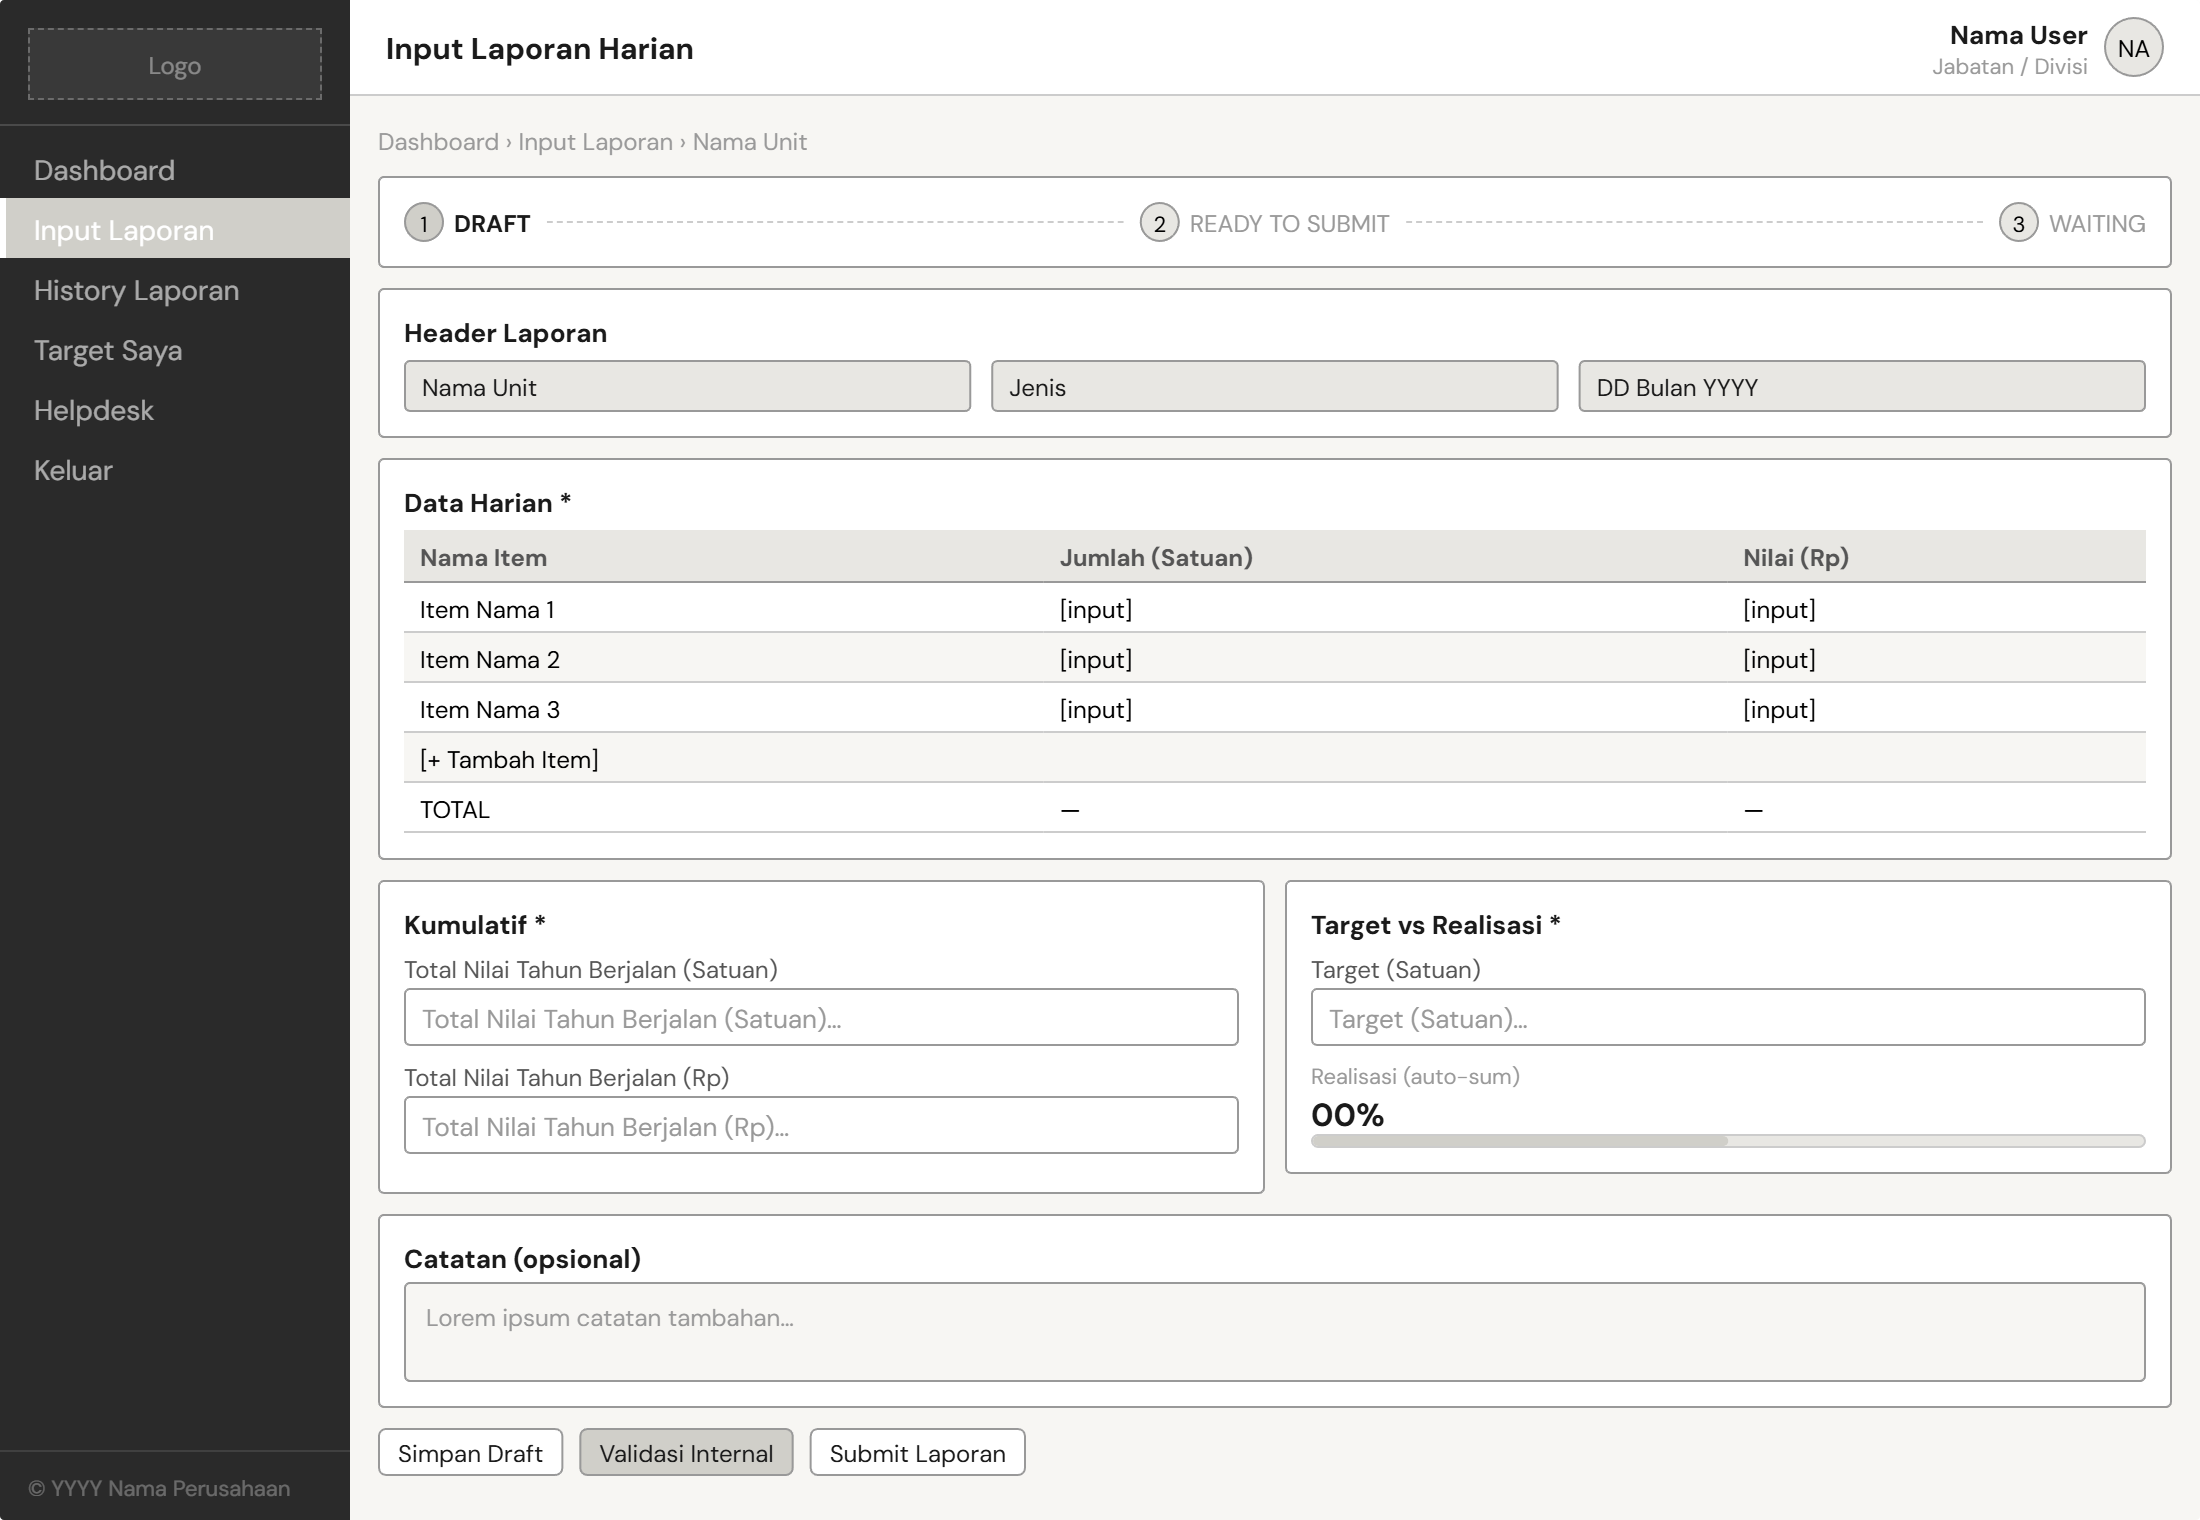
\includegraphics[width=0.85\textwidth]{figure/generated/lowfi-07-input-form-c.png}
    \caption{Desain \textit{Mid Fidelity} Halaman Input Laporan Harian Unit Angkutan Barang}
    \label{fig:3.lofi-07}
\end{figure}
Berdasarkan Gambar \ref{fig:3.lofi-07}, halaman ini digunakan User Unit untuk menginput data operasional harian berupa data per komoditi, data kumulatif, dan perbandingan target serta realisasi. Halaman ini dilengkapi indikator status laporan di bagian atas, kolom \textit{box} detail yang bersifat opsional, serta tiga tombol aksi yaitu Simpan Draft, Validasi Internal, dan Submit Laporan. \par

% \begin{figure}[H]
%     \centering
%     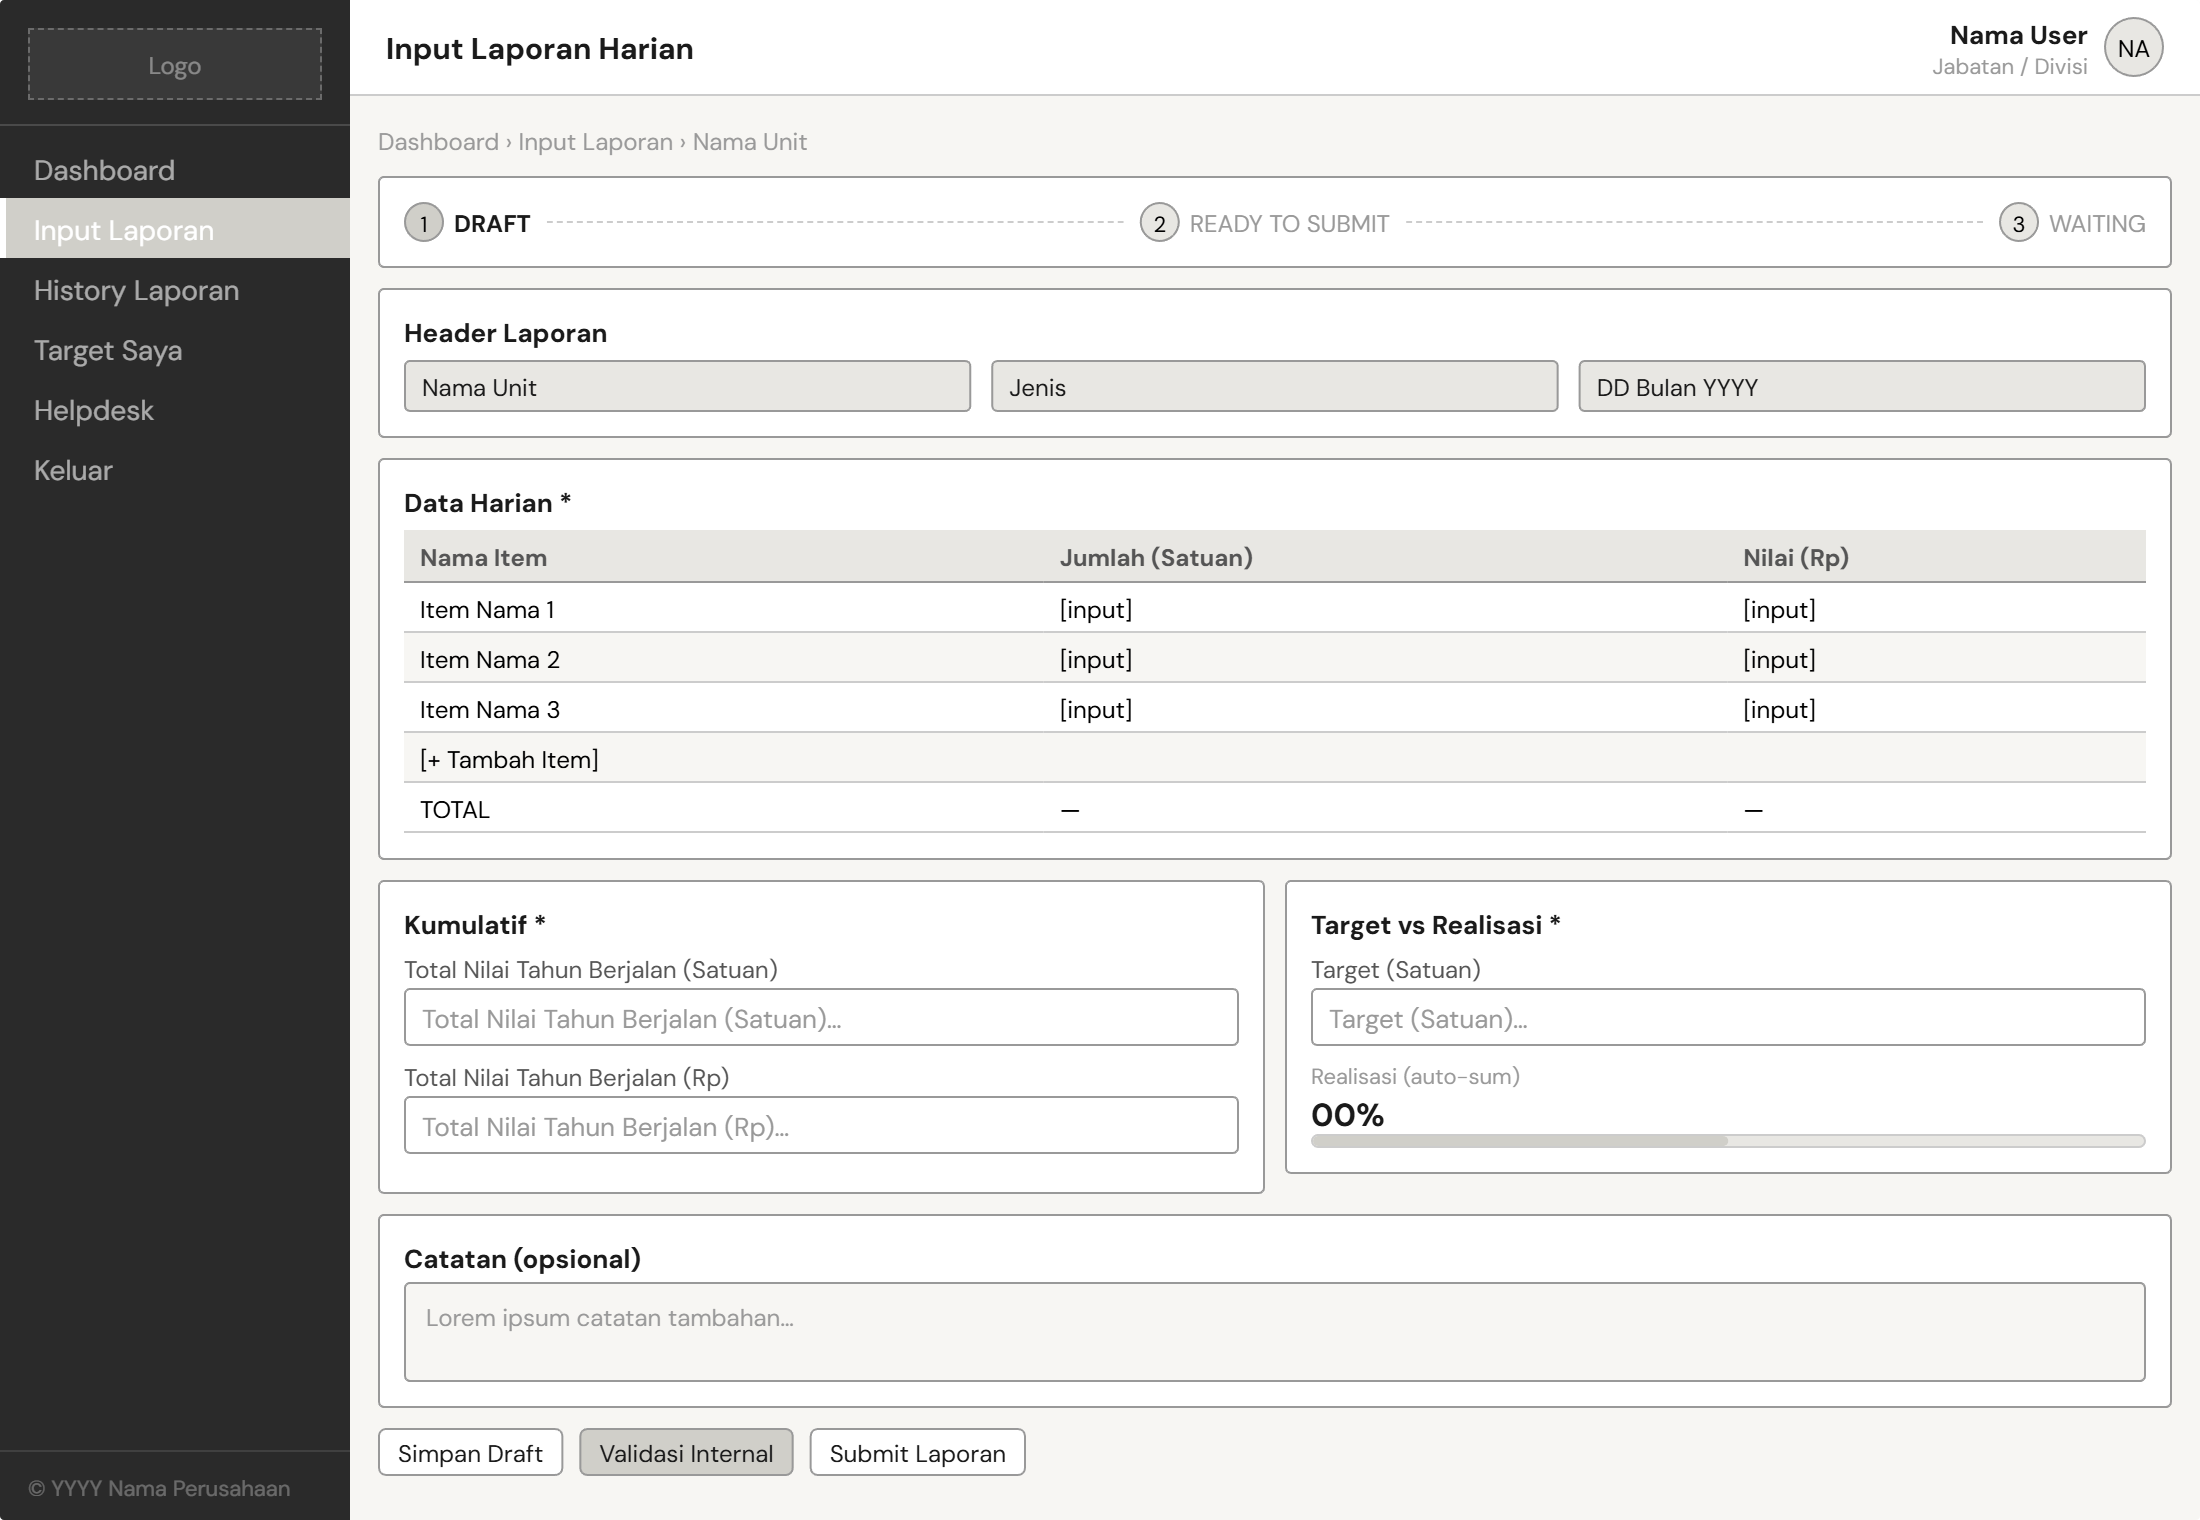
\includegraphics[width=0.85\textwidth]{figure/generated/lowfi-07-input-form-c.png}
%     \caption{Desain \textit{Mid Fidelity} Halaman Input Laporan Harian Unit Angkutan Barang}
%     \label{fig:3.lofi-07}
% \end{figure}

\textbf{13. Halaman Input Laporan Harian Unit KNA.} \par
\begin{figure}[H]
    \centering
    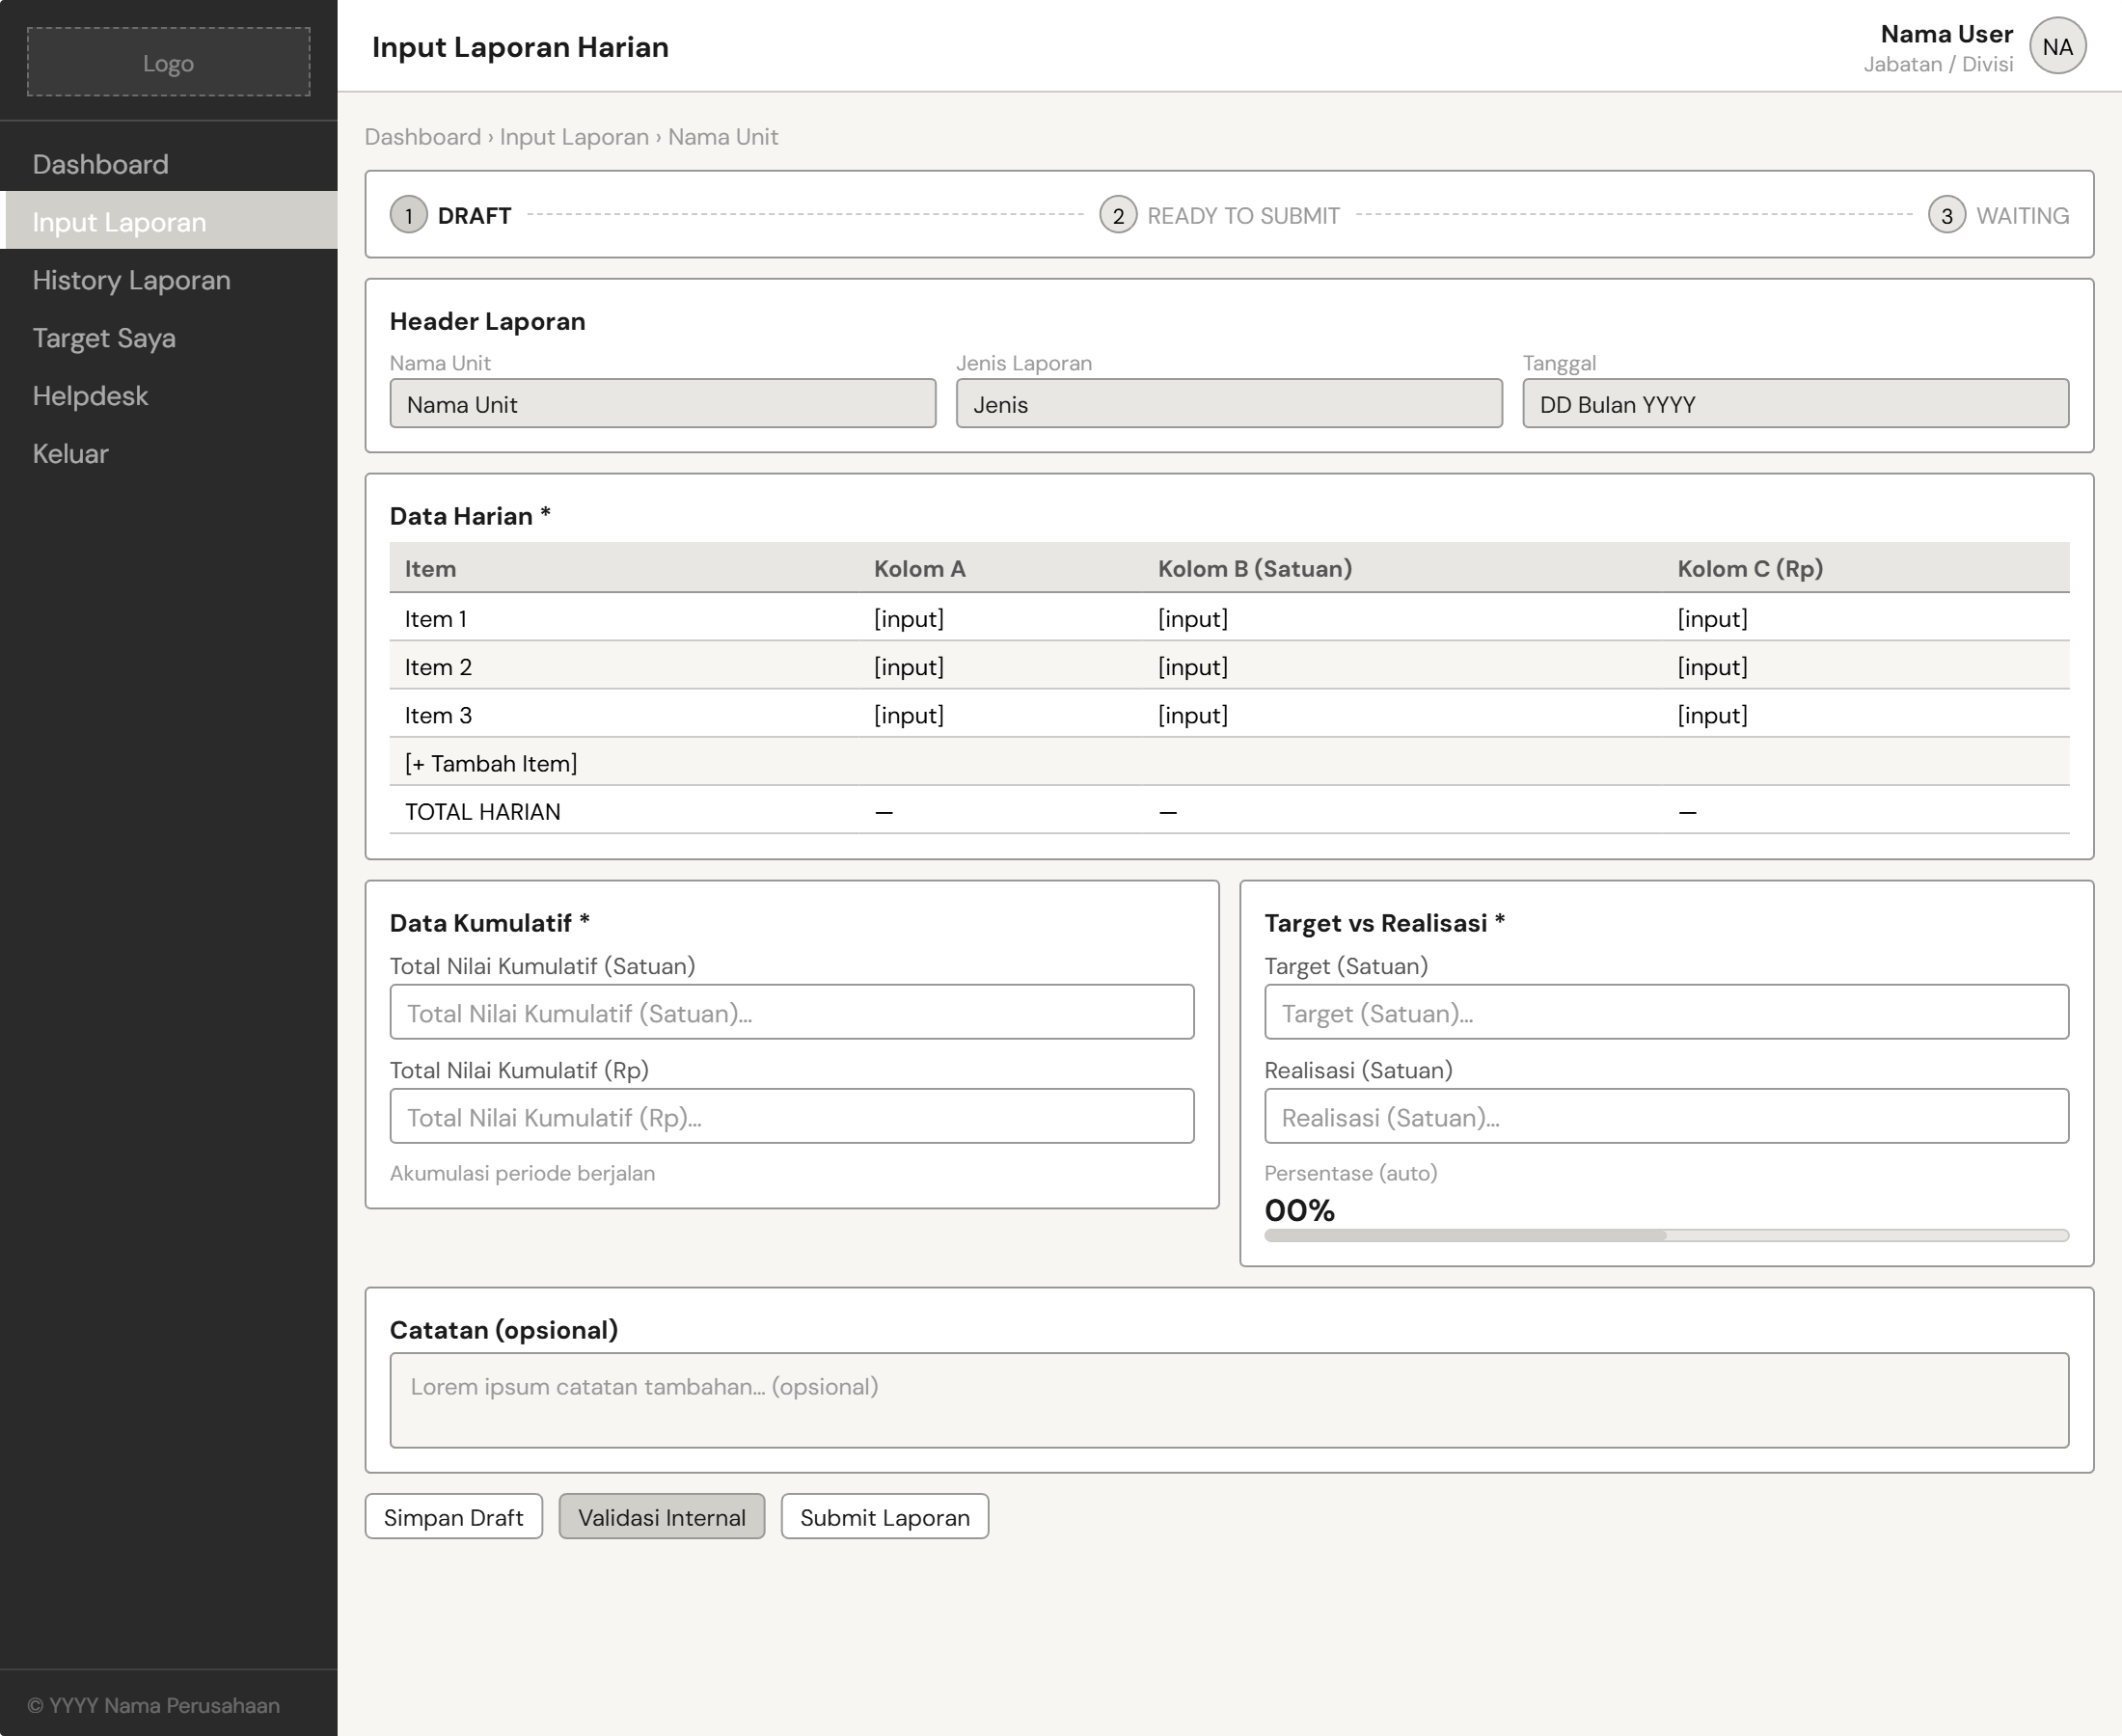
\includegraphics[width=0.85\textwidth]{figure/generated/lowfi-05-input-form-a.png}
    \caption{Desain \textit{Mid Fidelity} Halaman Input Laporan Harian Unit KNA}
    \label{fig:3.lofi-05}
\end{figure}
Rancangan halaman input laporan harian unit KNA dapat dilihat pada Gambar \ref{fig:3.lofi-05} diatas Halaman input laporan harian unit KNA merupakan halaman yang digunakan User Unit KNA untuk menginput data kontrak harian yang terbagi ke dalam dua sub-bagian, yaitu data ROW dan Non-ROW, beserta perbandingan target RKAD dan realisasi. Halaman ini menggunakan label RKAD sebagai acuan target yang membedakannya dari unit lain, dilengkapi kolom \textit{box} detail opsional dan tiga tombol aksi di bagian bawah. 


\textbf{14. Halaman Input Laporan Harian Unit Angkutan Penumpang.} \par
Rancangan halaman input laporan harian unit Angkutan Penumpang dapat dilihat pada Gambar \ref{fig:3.lofi-06}. Halaman input laporan harian unit Angkutan Penumpang merupakan halaman yang digunakan User Unit untuk menginput data jumlah penumpang dan pendapatan per kereta api yang beroperasi pada hari tersebut. Halaman ini memuat tabel data harian per KA, bagian kumulatif tahun berjalan, perbandingan target dan realisasi penumpang, serta kolom \textit{box} detail opsional dan tiga tombol aksi.

\begin{figure}[H]
    \centering
    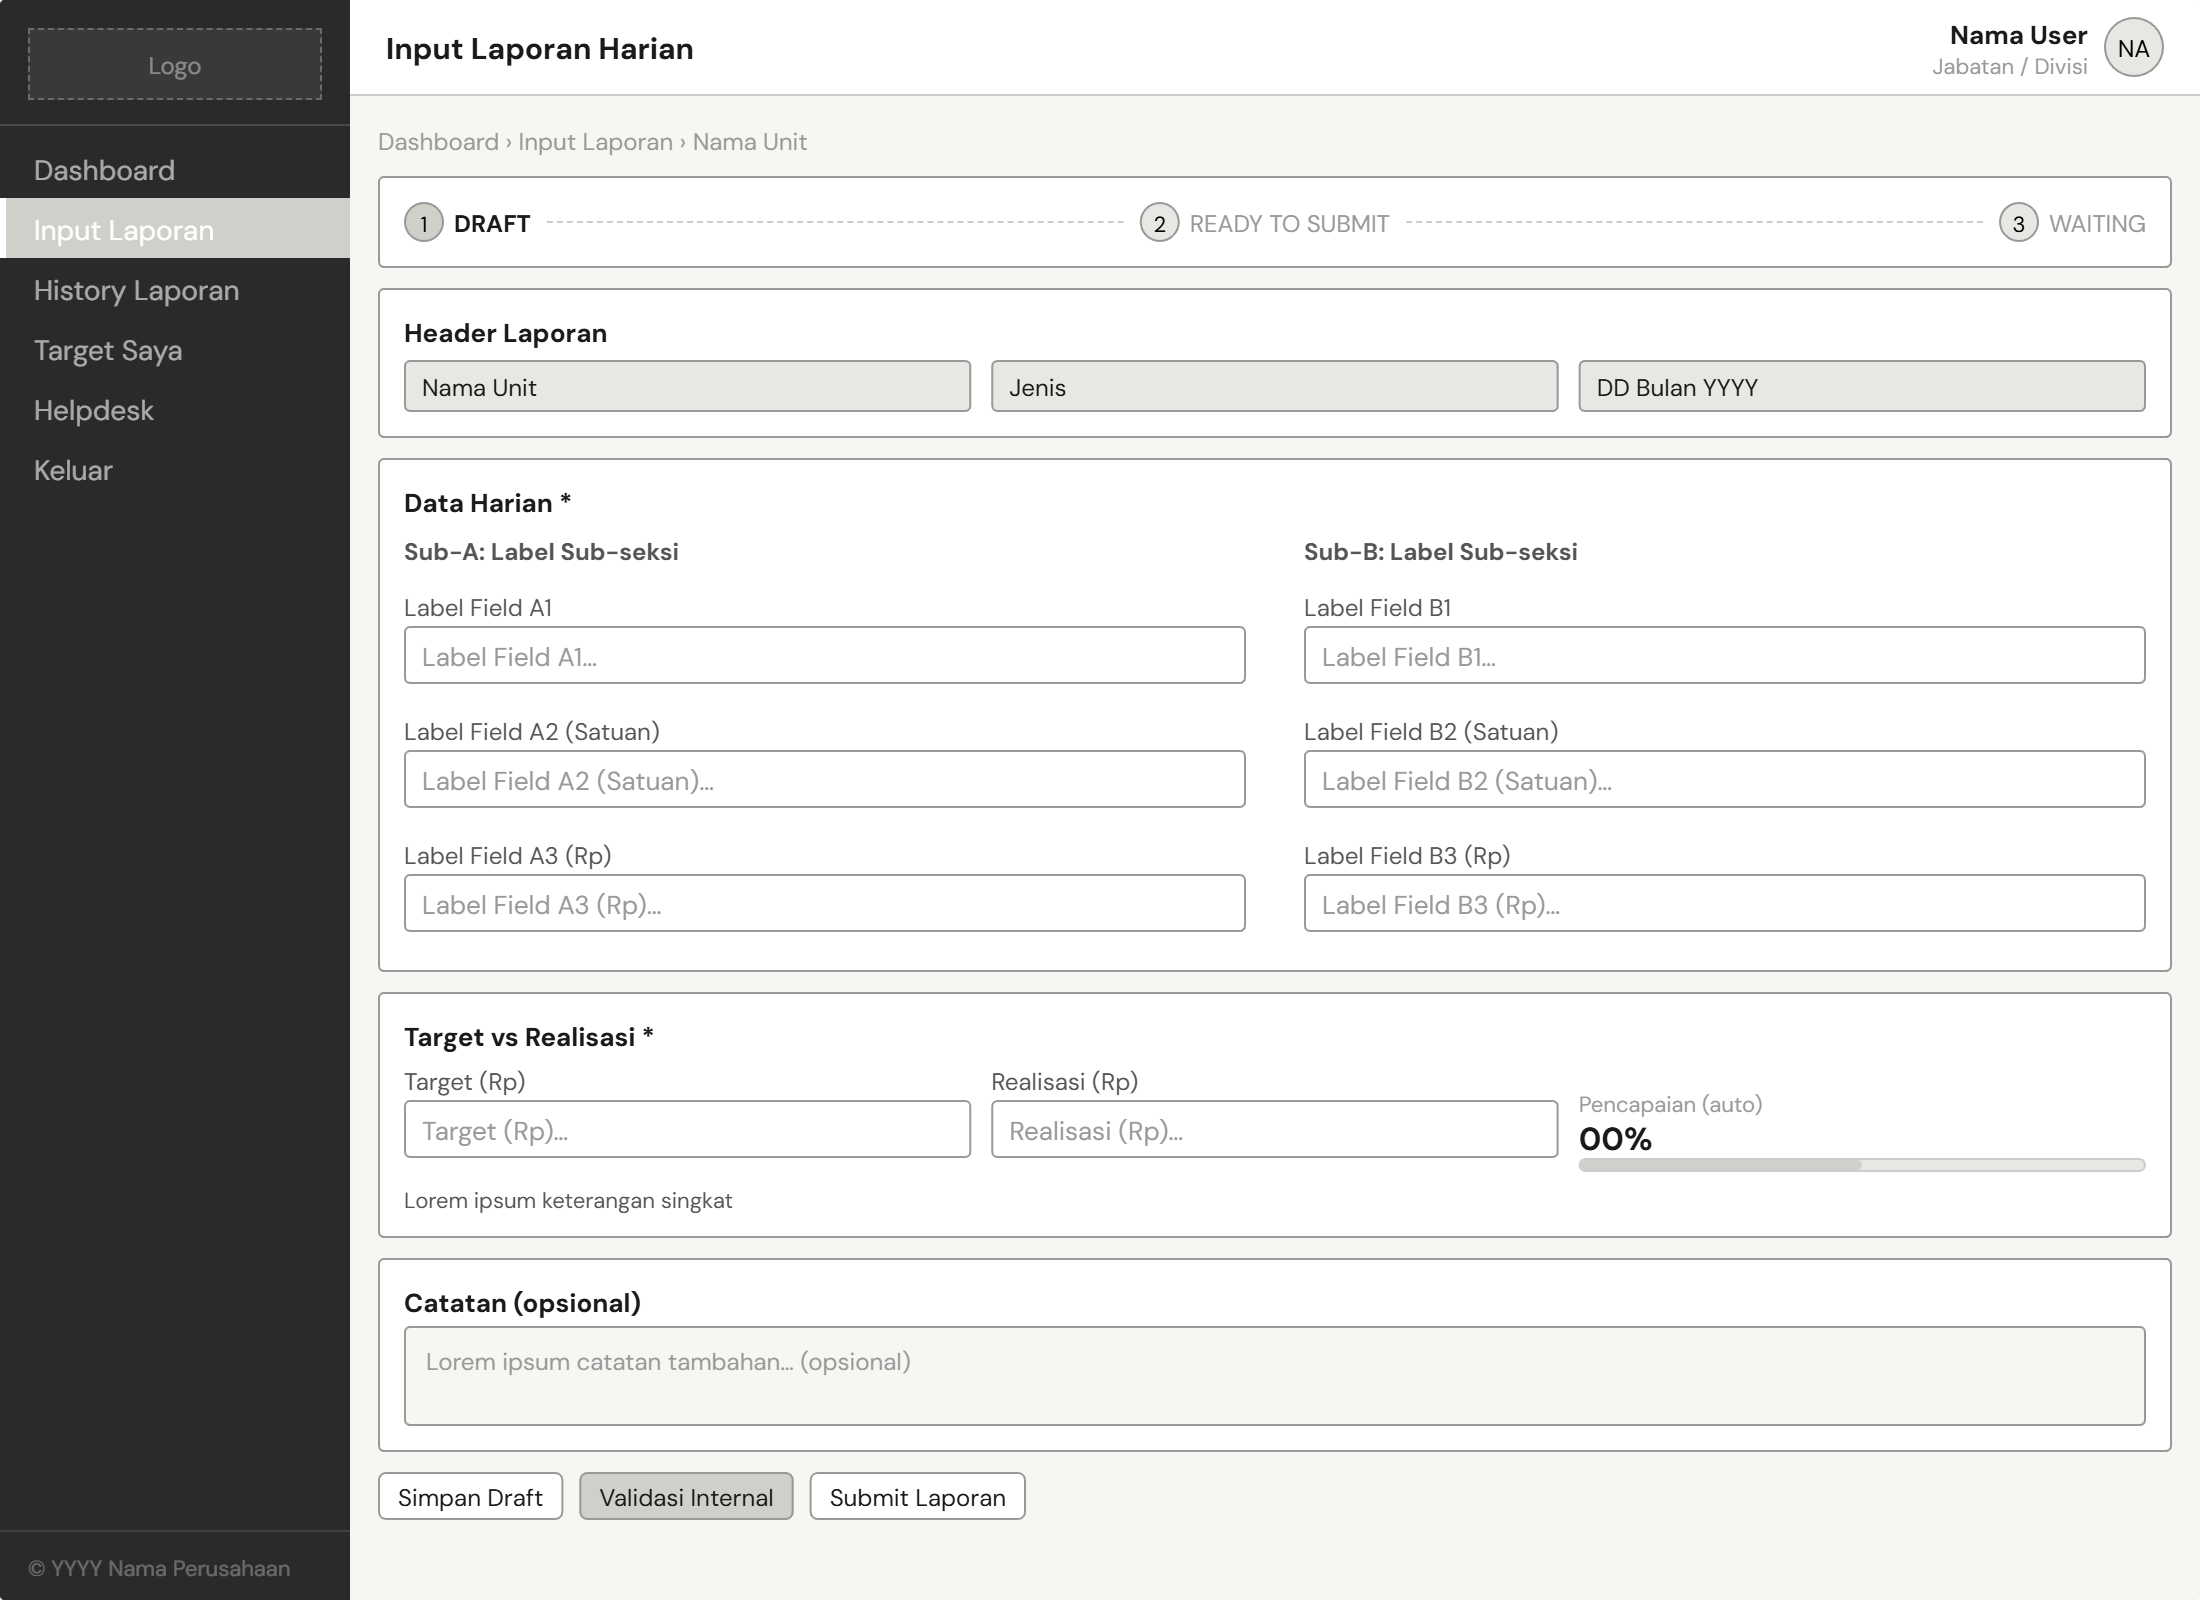
\includegraphics[width=0.85\textwidth]{figure/generated/lowfi-06-input-form-b.png}
    \caption{Desain \textit{Mid Fidelity} Halaman Input Laporan Harian Unit Angkutan Penumpang}
    \label{fig:3.lofi-06}
\end{figure}

\textbf{15. Halaman Input Laporan Harian Unit Keuangan.} \par
Rancangan halaman input laporan harian unit Keuangan ditunjukkan pada Gambar \ref{fig:3.lofi-08}.
Berdasarkan Gambar \ref{fig:3.lofi-08}, halaman ini digunakan User Unit untuk menginput data keuangan harian yang terdiri dari tiga bagian utama, yaitu Data Harian dengan kolom Nilai A, Nilai B, dan Nilai C yang dihitung secara otomatis oleh sistem, bagian Kumulatif yang menampilkan total nilai kumulatif beserta total nilai C kumulatif secara otomatis, serta bagian Target vs Realisasi yang dilengkapi indikator persentase pencapaian. Halaman ini juga menyediakan kolom catatan opsional dan tiga tombol aksi Simpan Draft, Validasi Internal, dan Submit Laporan di bagian bawah. \par

\begin{figure}[H]
    \centering
    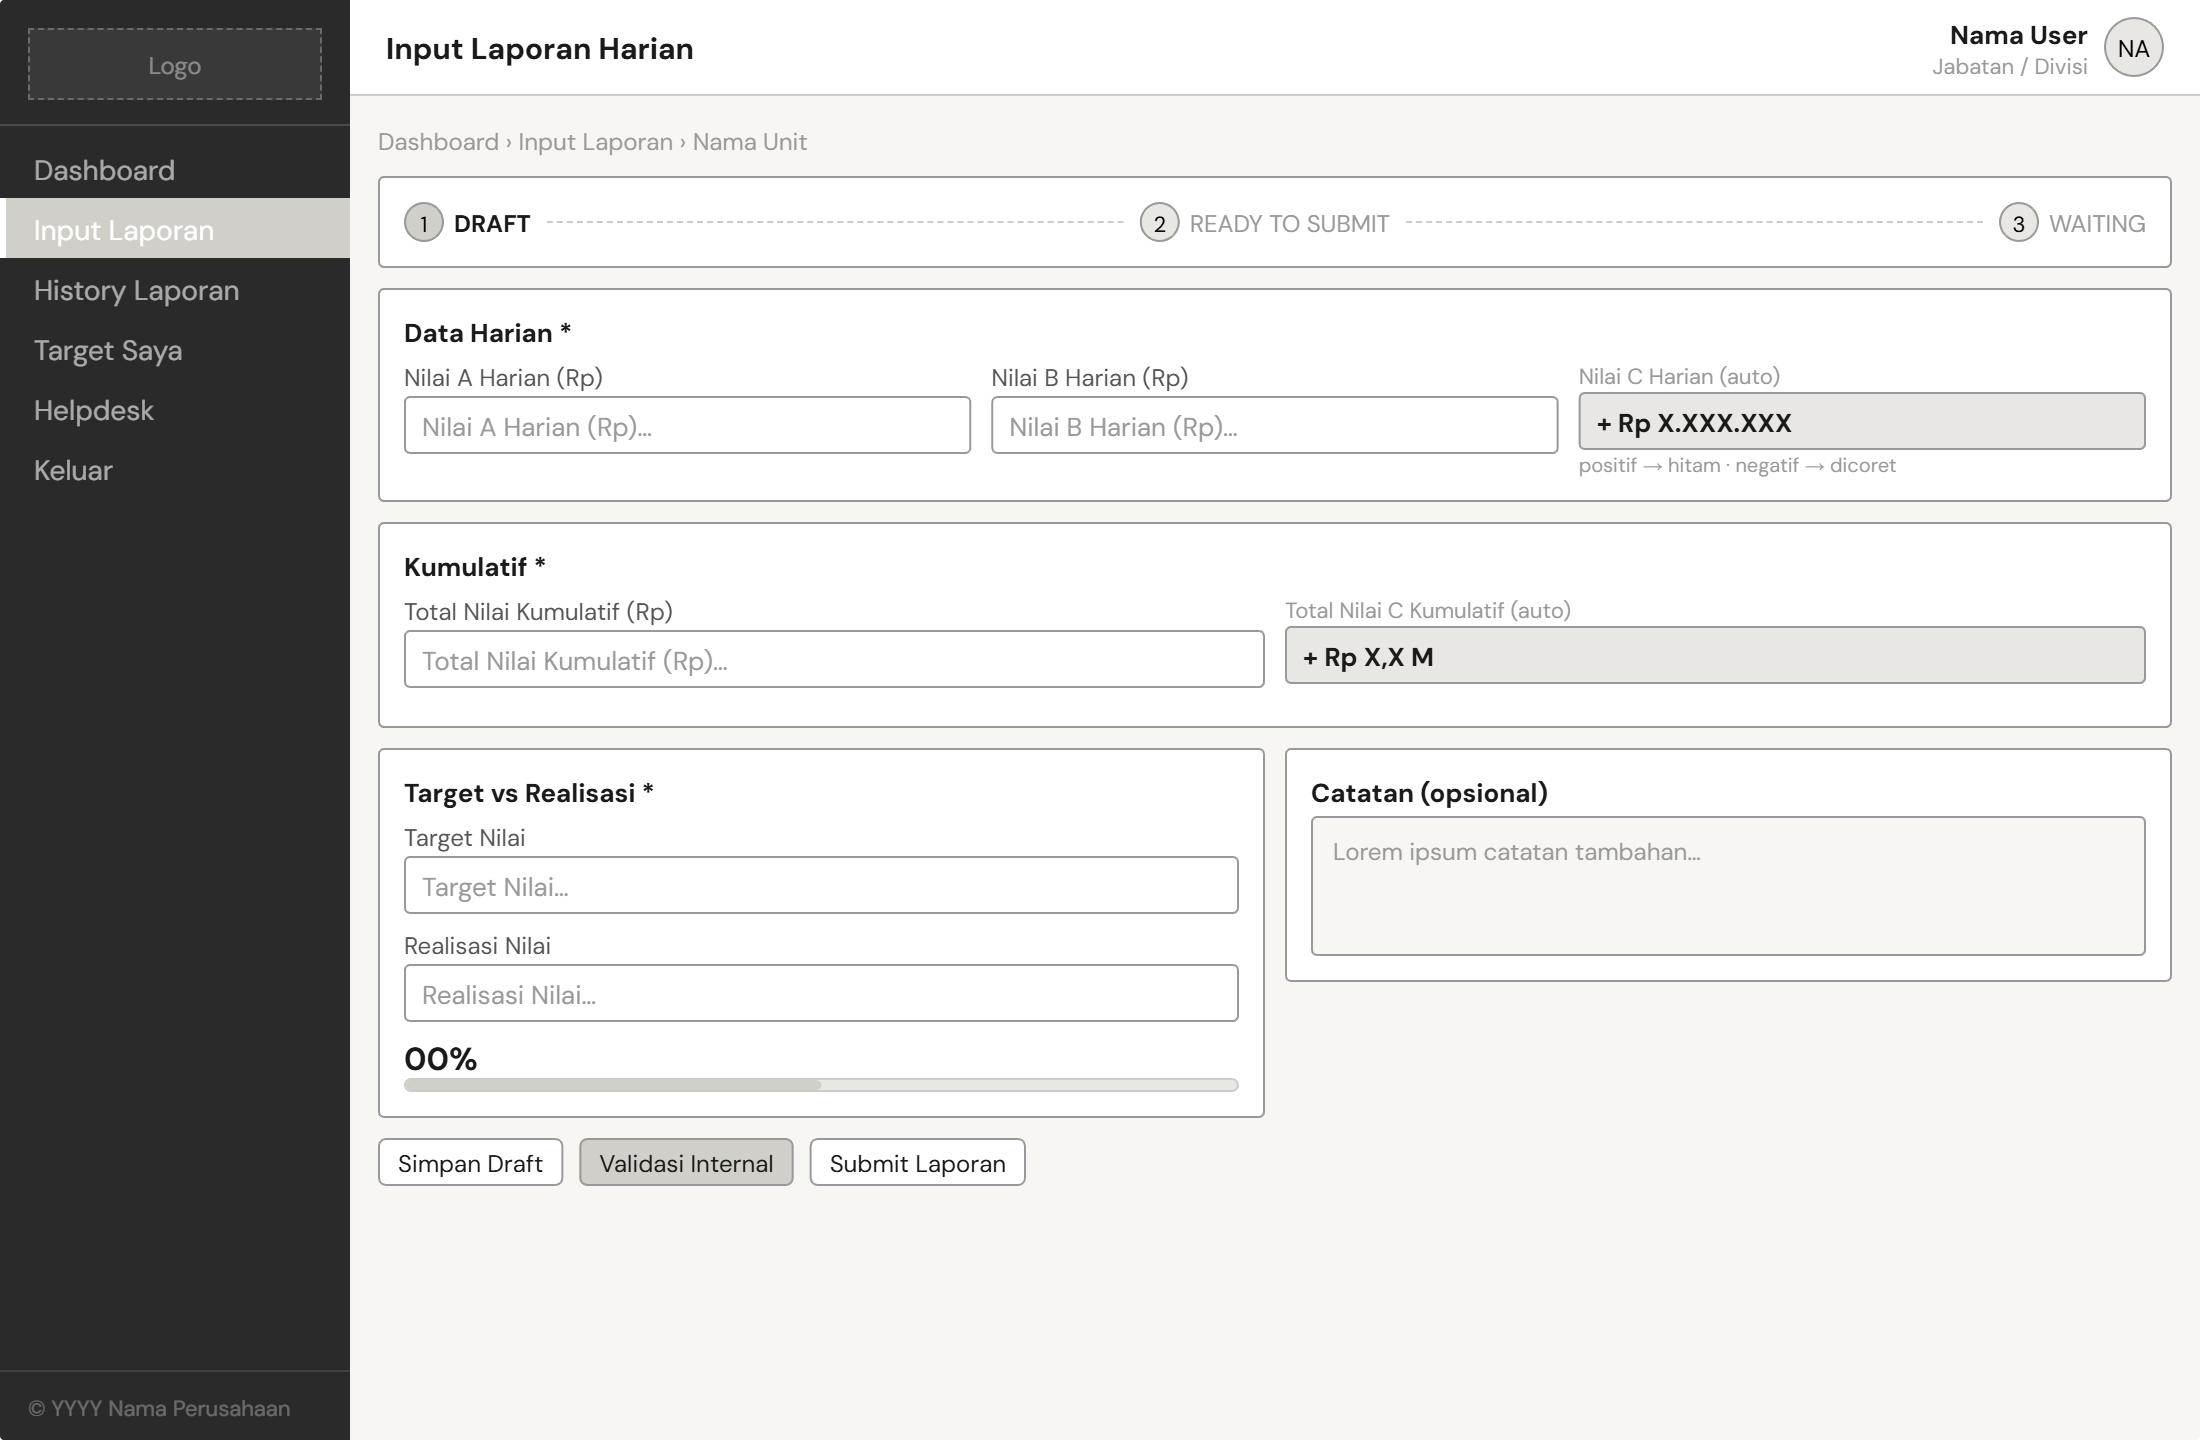
\includegraphics[width=0.85\textwidth]{figure/generated/lowfi-08-input-form-d.png}
    \caption{Desain \textit{Mid Fidelity} Halaman Input Laporan Harian Unit Keuangan}
    \label{fig:3.lofi-08}
\end{figure}


\textbf{16. Halaman History Laporan User Unit.} \par
\begin{figure}[H]
    \centering
    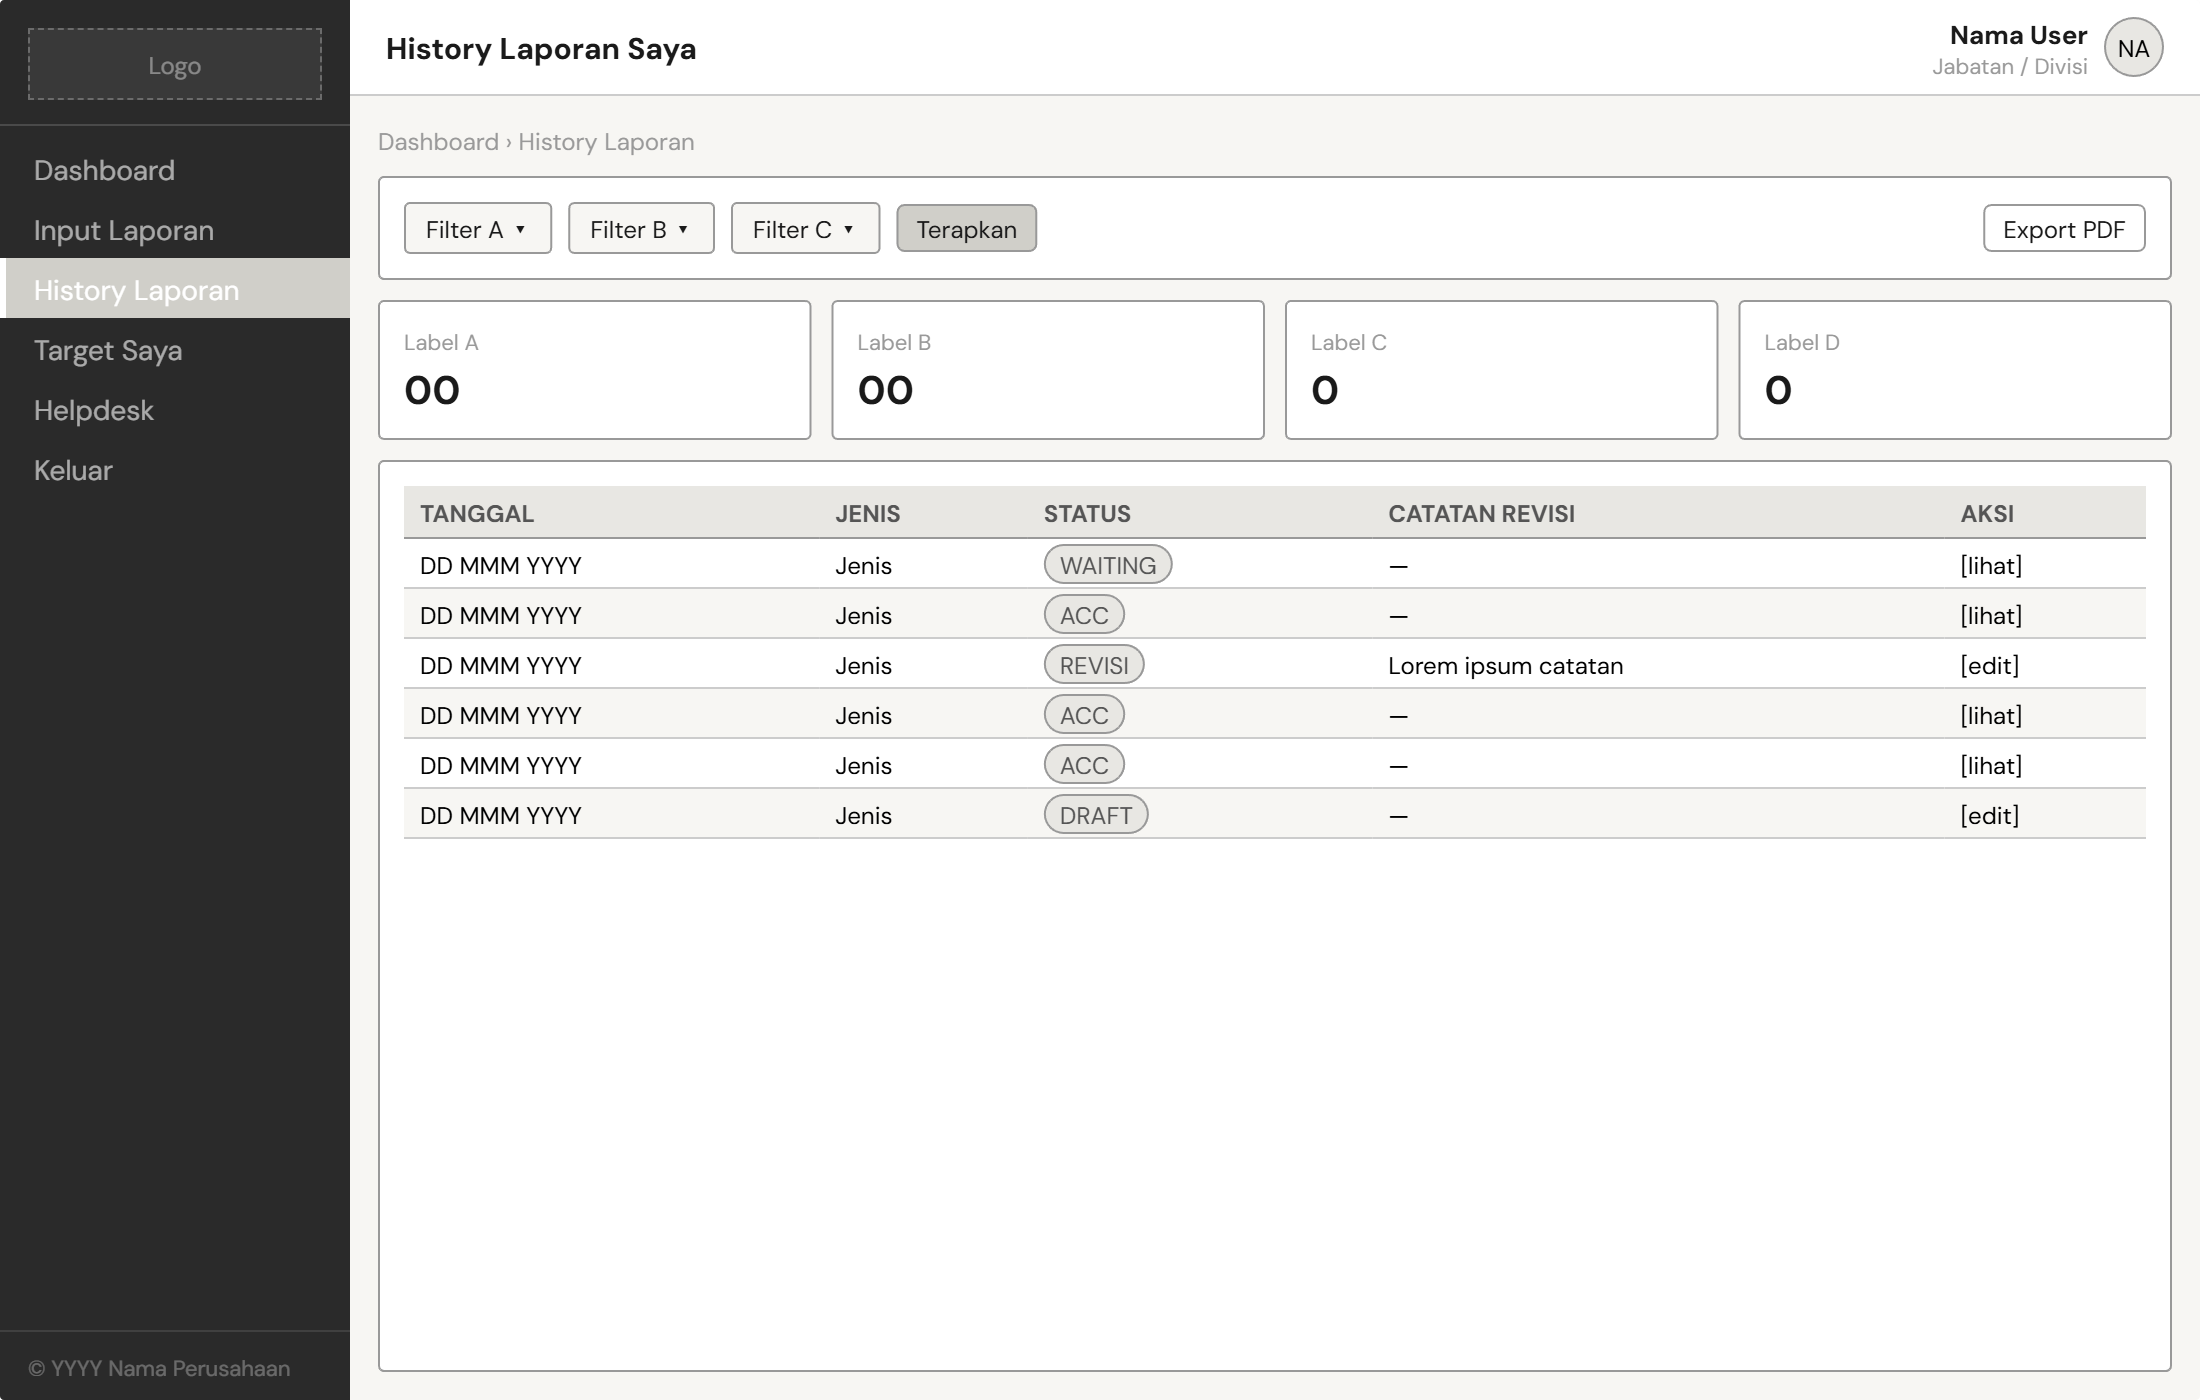
\includegraphics[width=0.85\textwidth]{figure/generated/lowfi-19b-history-laporan-user.png}
    \caption{Desain \textit{Mid Fidelity} Halaman History Laporan User Unit}
    \label{fig:3.lofi-19b}
\end{figure}
Rancangan halaman history laporan User Unit dapat dilihat pada Gambar \ref{fig:3.lofi-19b} diatas. Halaman history laporan User Unit merupakan halaman yang menyediakan rekam jejak seluruh laporan yang pernah dikirimkan oleh unit yang bersangkutan beserta status terkininya. Halaman ini memuat kartu ringkasan jumlah laporan per status, filter berdasarkan bulan, tahun, dan status, serta tabel laporan yang menampilkan tanggal, jenis, status, catatan revisi, dan tombol aksi. 

% \begin{figure}[H]
%     \centering
%     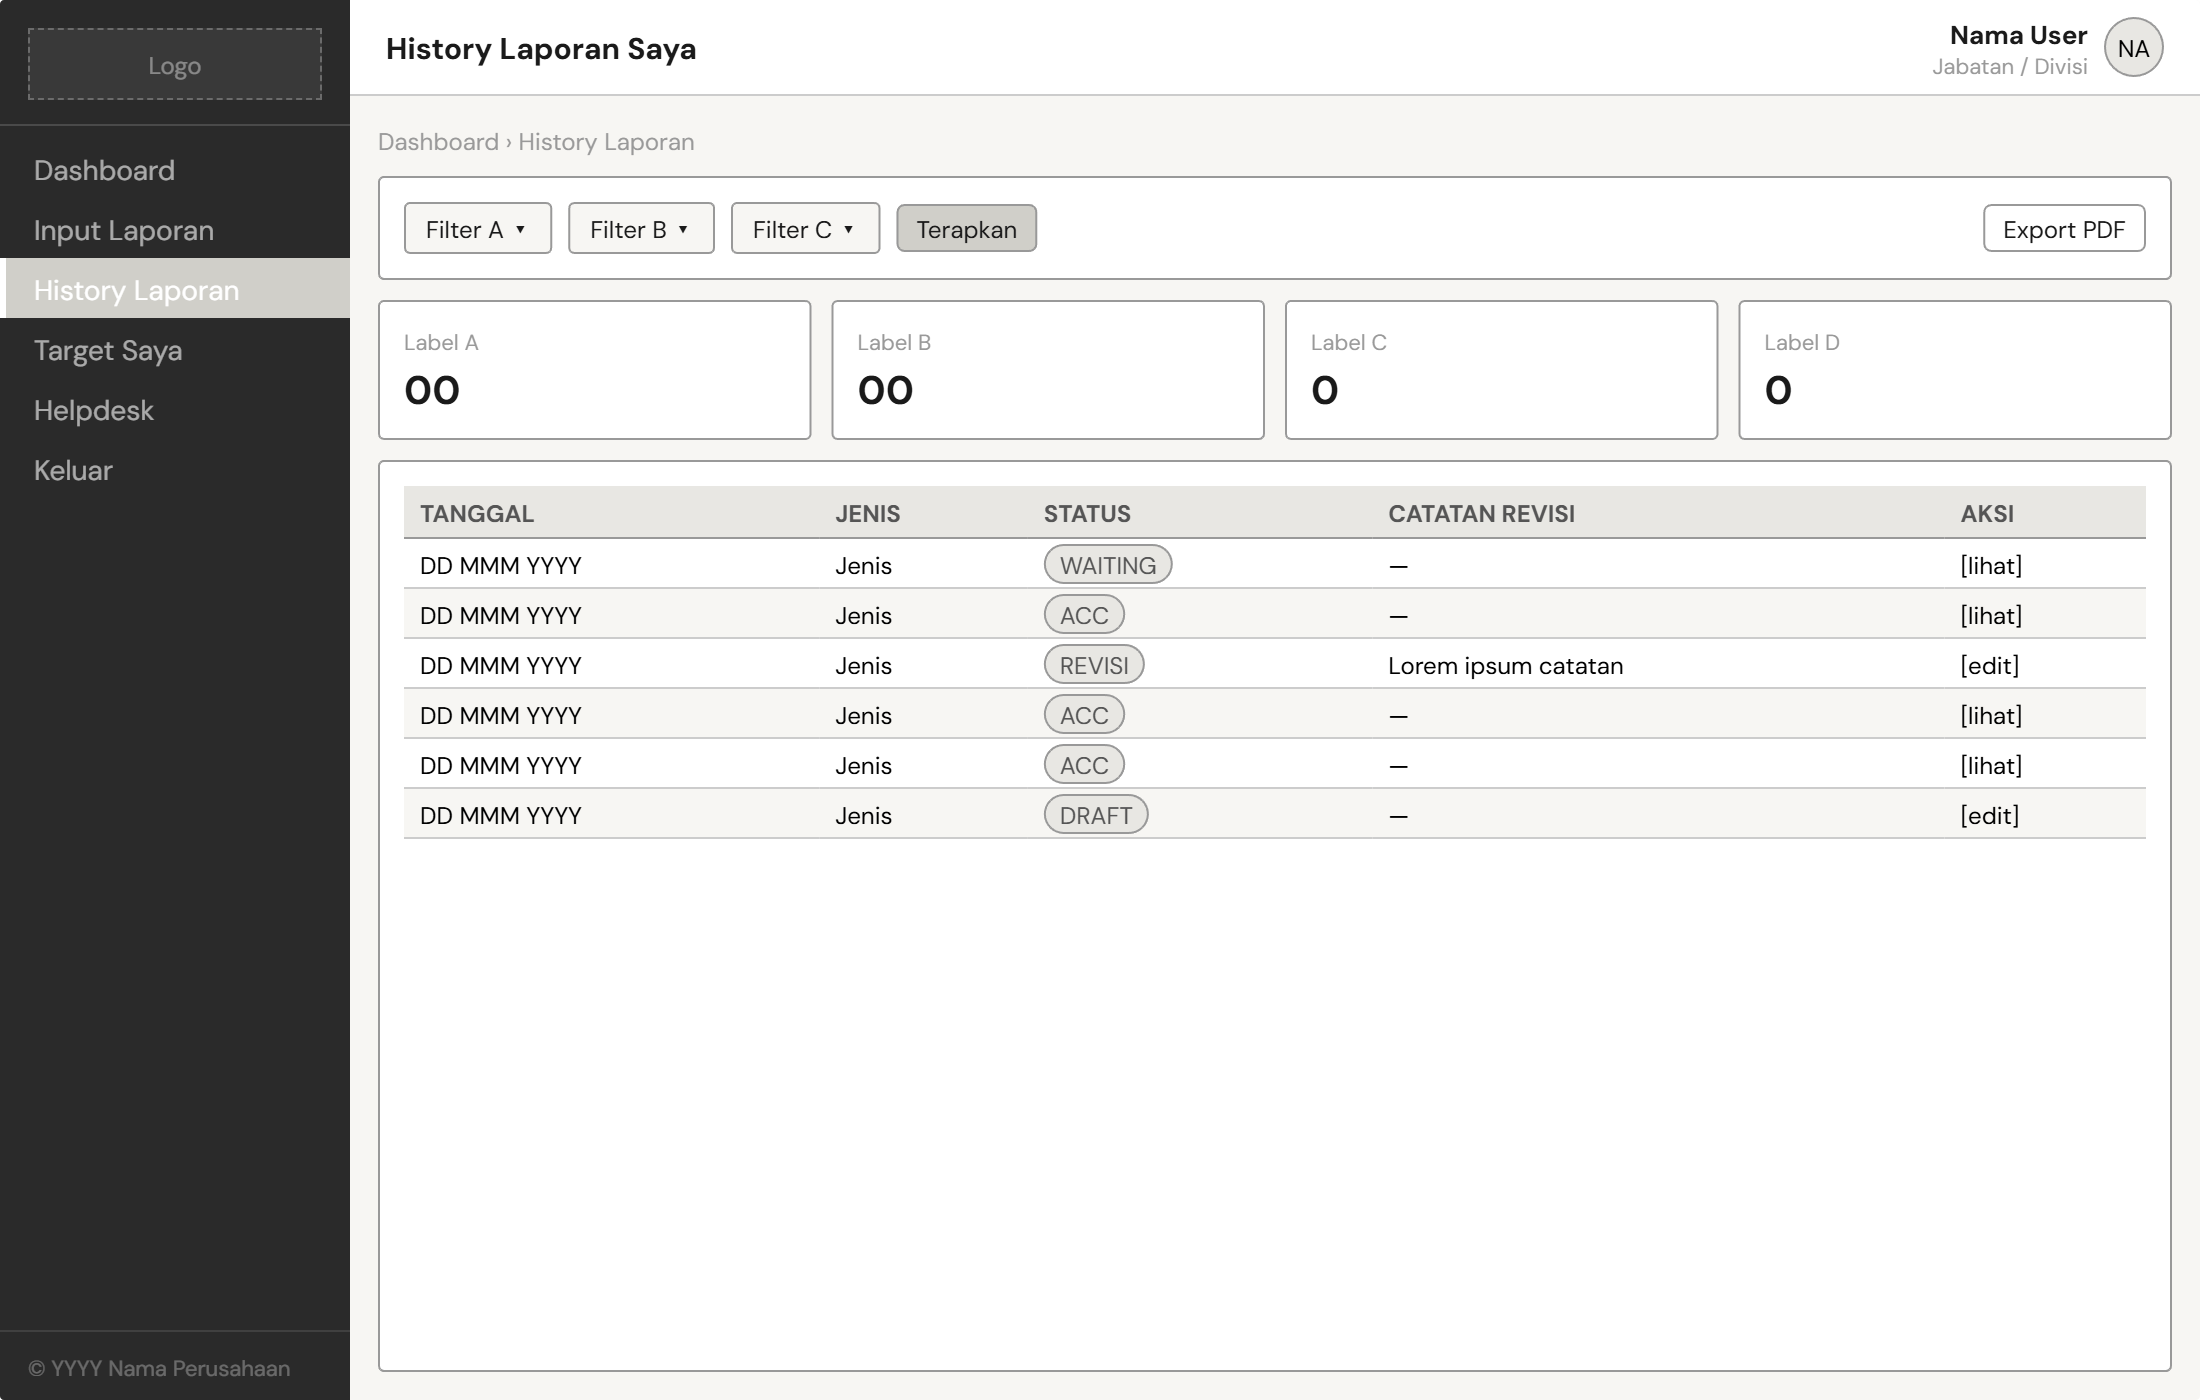
\includegraphics[width=0.85\textwidth]{figure/generated/lowfi-19b-history-laporan-user.png}
%     \caption{Desain \textit{Mid Fidelity} Halaman History Laporan User Unit}
%     \label{fig:3.lofi-19b}
% \end{figure}

\textbf{17. Halaman Helpdesk \& Bantuan.} \par
Halaman helpdesk dan bantuan merupakan halaman yang digunakan User Unit dan Admin Global untuk mengajukan tiket permintaan bantuan kepada pihak yang berwenang tanpa perlu berkomunikasi di luar sistem. Halaman ini menyediakan tiga pilihan jenis tiket yaitu TOKEN, ISSUE, dan REVISION, dilengkapi kolom deskripsi wajib dan konfirmasi pengiriman setelah tiket berhasil dikirimkan. Rancangan halaman helpdesk dan bantuan dapat dilihat pada Gambar \ref{fig:3.lofi-10} berikut.

\begin{figure}[H]
    \centering
    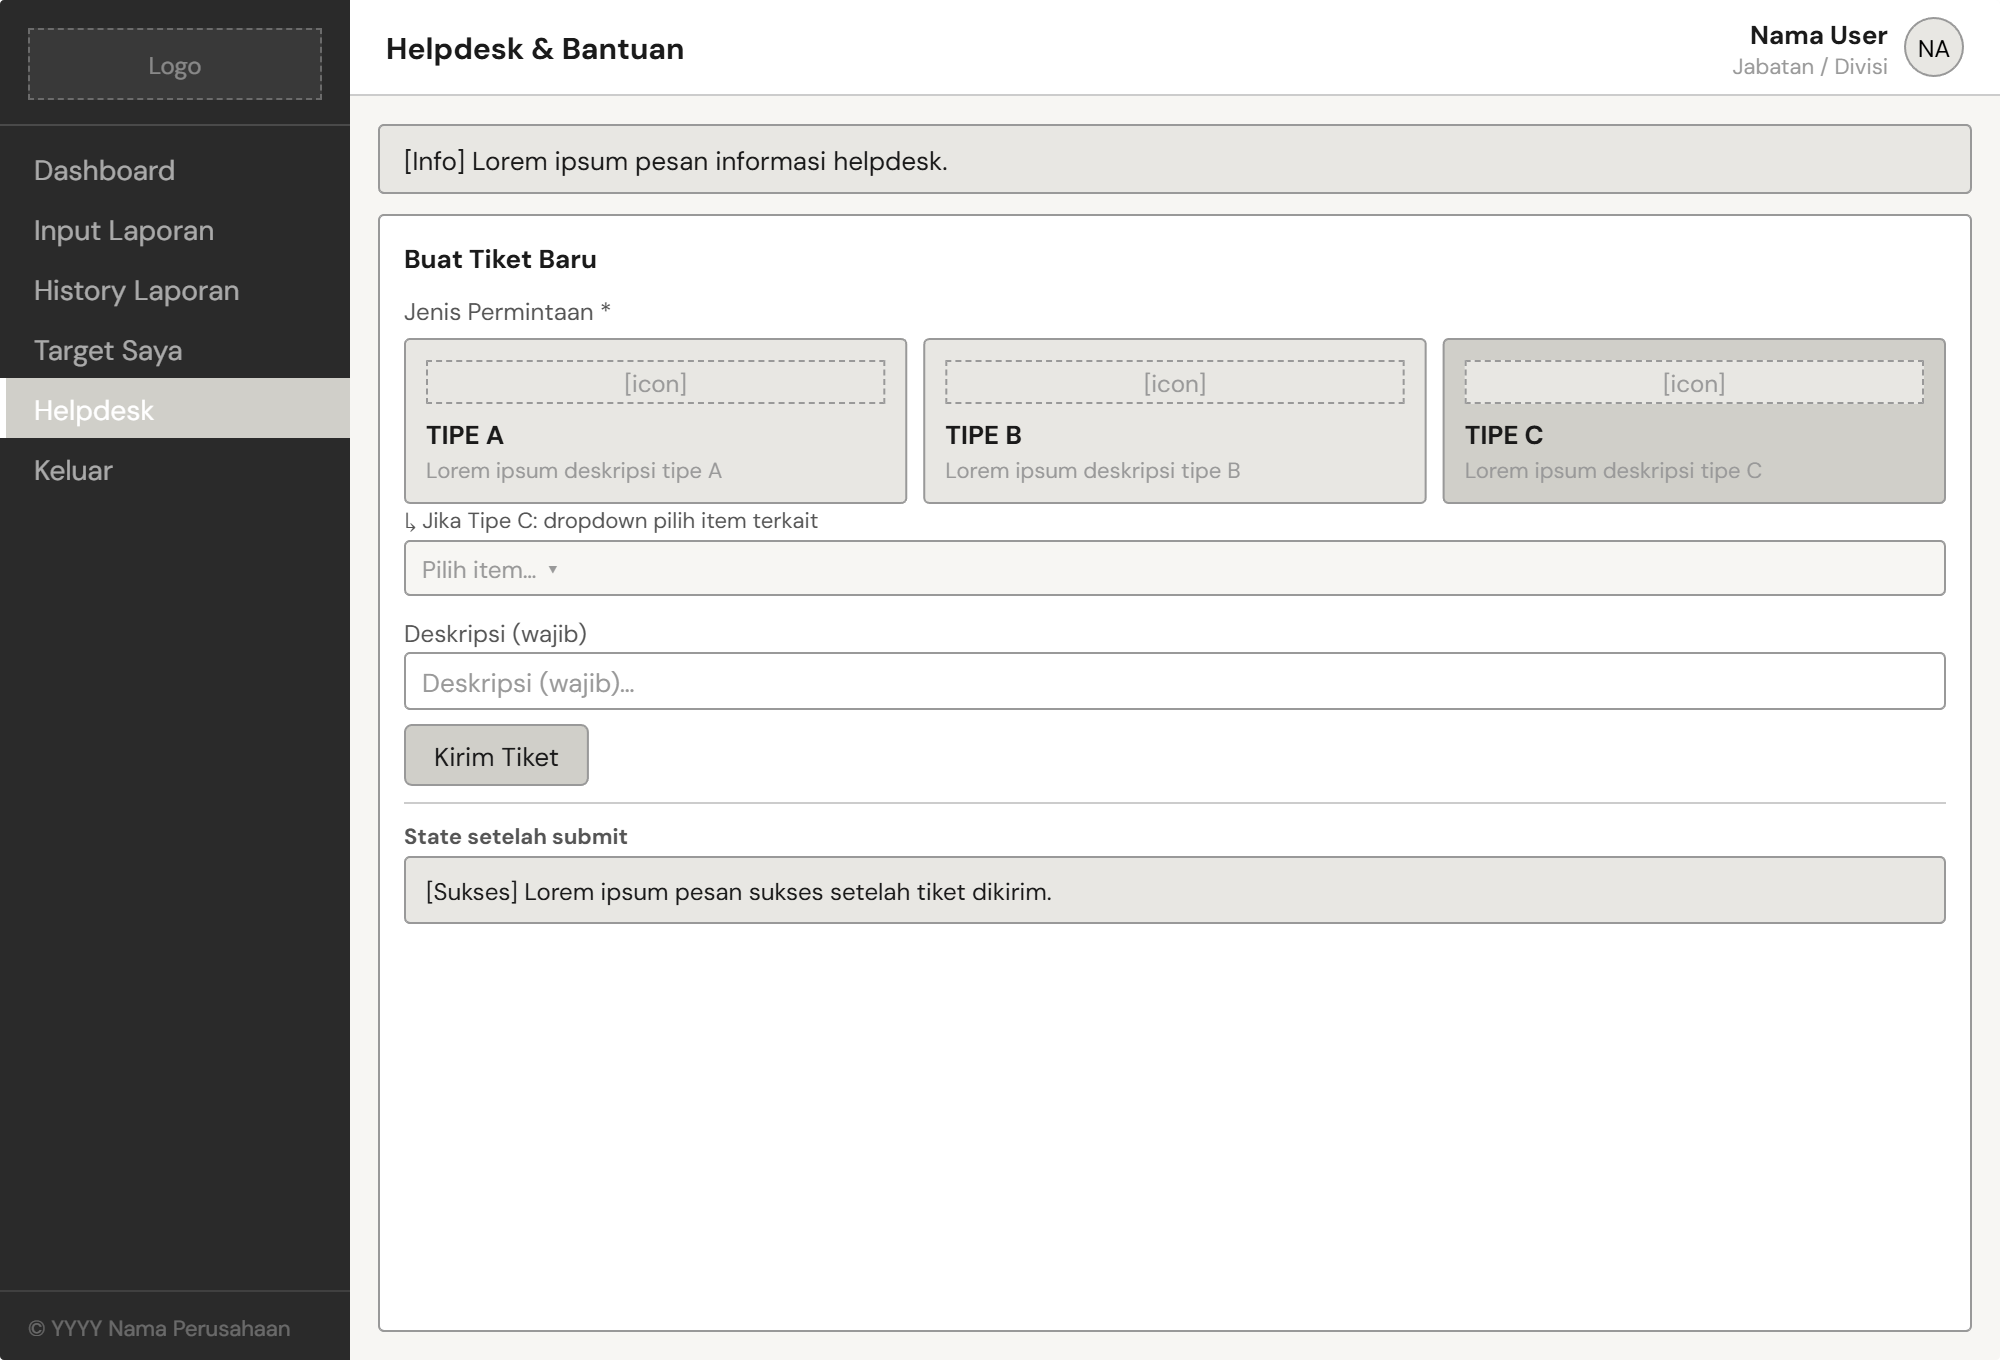
\includegraphics[width=0.85\textwidth]{figure/generated/lowfi-10-helpdesk-ajukan-tiket.png}
    \caption{Desain \textit{Mid Fidelity} Halaman Helpdesk \& Bantuan}
    \label{fig:3.lofi-10}
\end{figure}

\textbf{18. Halaman Dashboard IT Support.} \par
Rancangan halaman dashboard IT Support ditunjukkan pada Gambar \ref{fig:3.lofi-12}.

\begin{figure}[H]
    \centering
    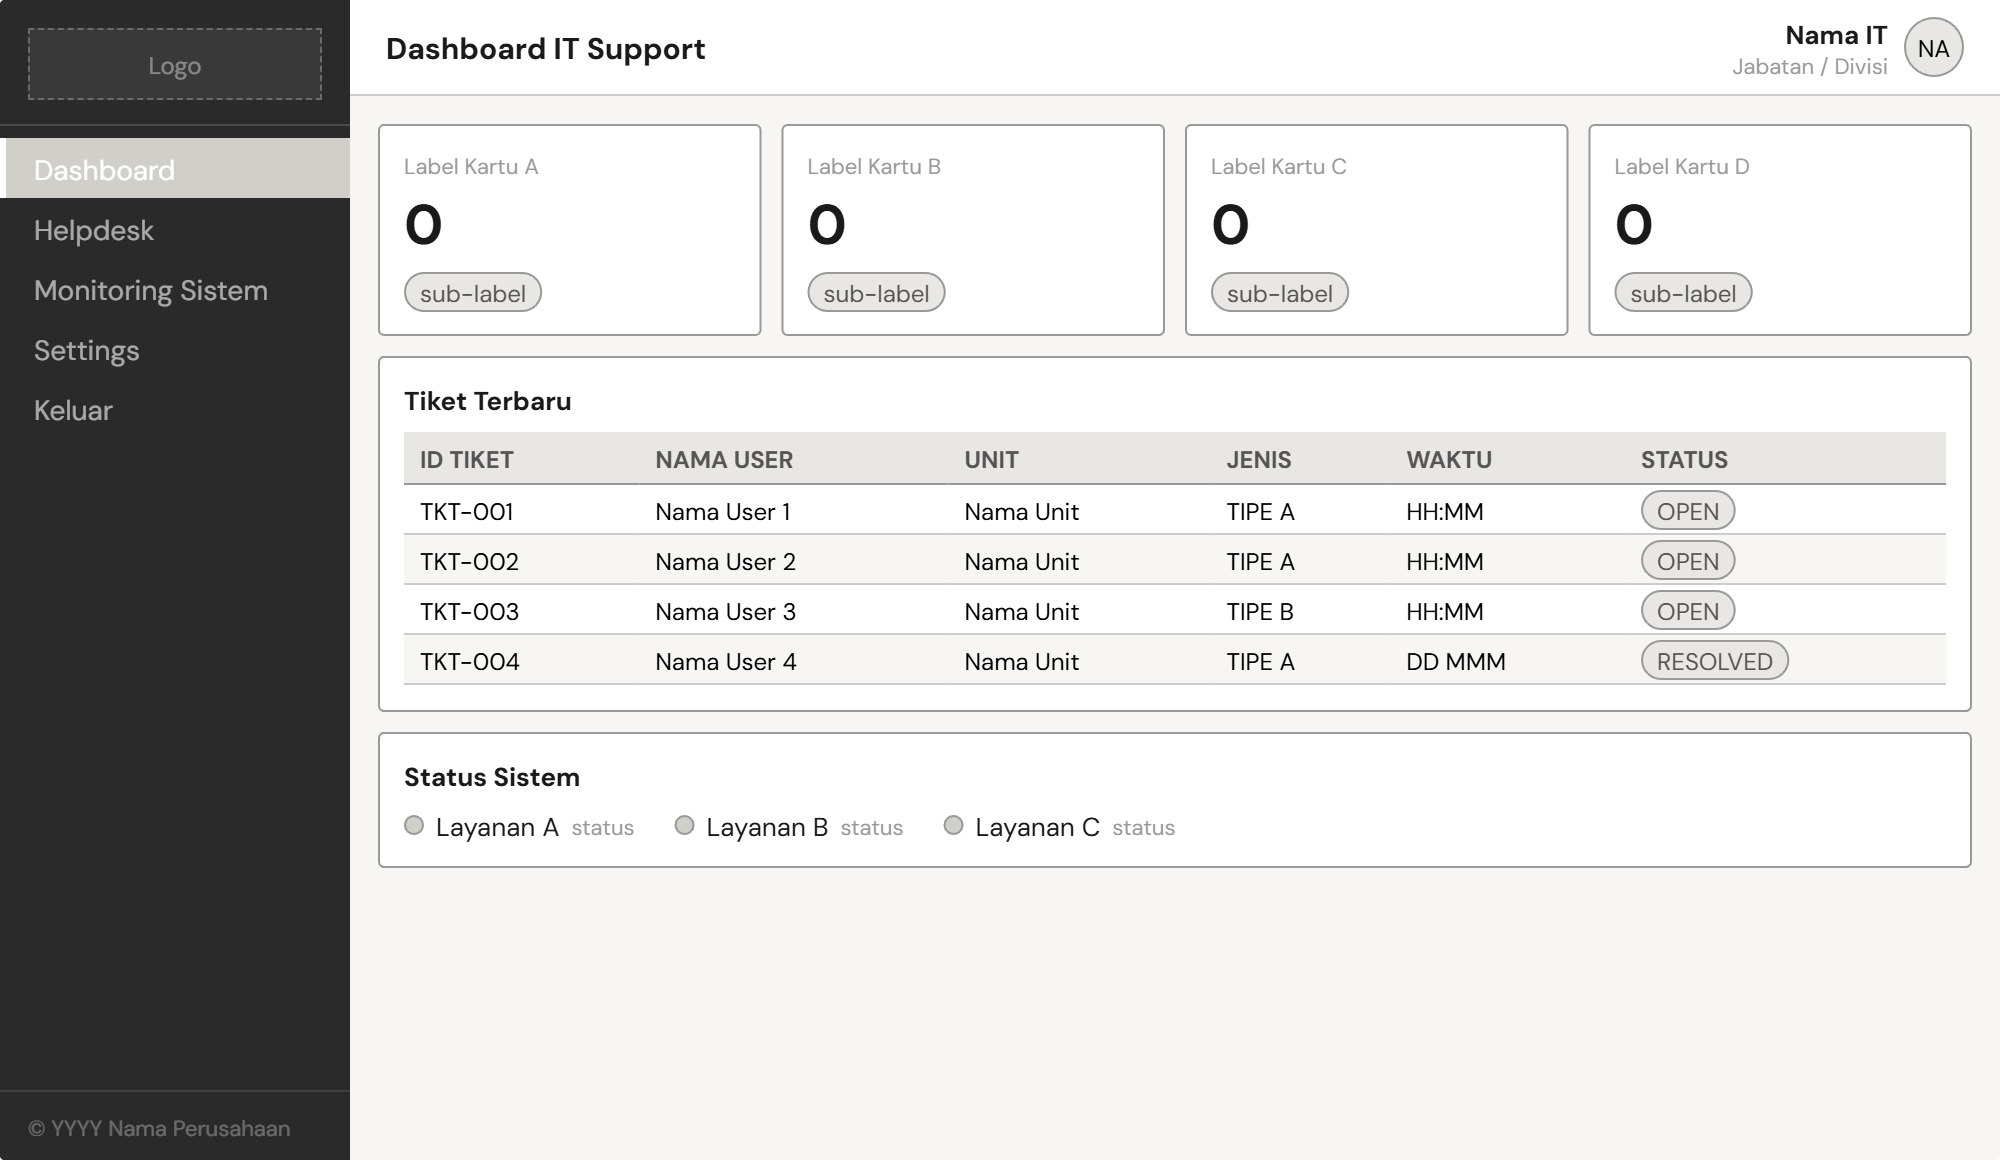
\includegraphics[width=0.85\textwidth]{figure/generated/lowfi-12-dashboard-it-support.png}
    \caption{Desain \textit{Mid Fidelity} Halaman Dashboard IT Support}
    \label{fig:3.lofi-12}
\end{figure}

Berdasarkan Gambar \ref{fig:3.lofi-12}, halaman ini merupakan halaman utama yang ditampilkan kepada IT Support setelah masuk dan dirancang untuk memberikan gambaran cepat mengenai kondisi tiket dan kesehatan sistem. Halaman ini memuat kartu ringkasan jumlah tiket TOKEN dan ISSUE yang \textit{pending}, tabel tiket terbaru, serta panel Status Sistem yang menampilkan kondisi \textit{Backend}, \textit{Database}, dan WhatsApp Gateway secara \textit{real-time}. \par

\textbf{19. Halaman Manajemen Helpdesk: Daftar Tiket (IT Support).} \par
\begin{figure}[H]
    \centering
    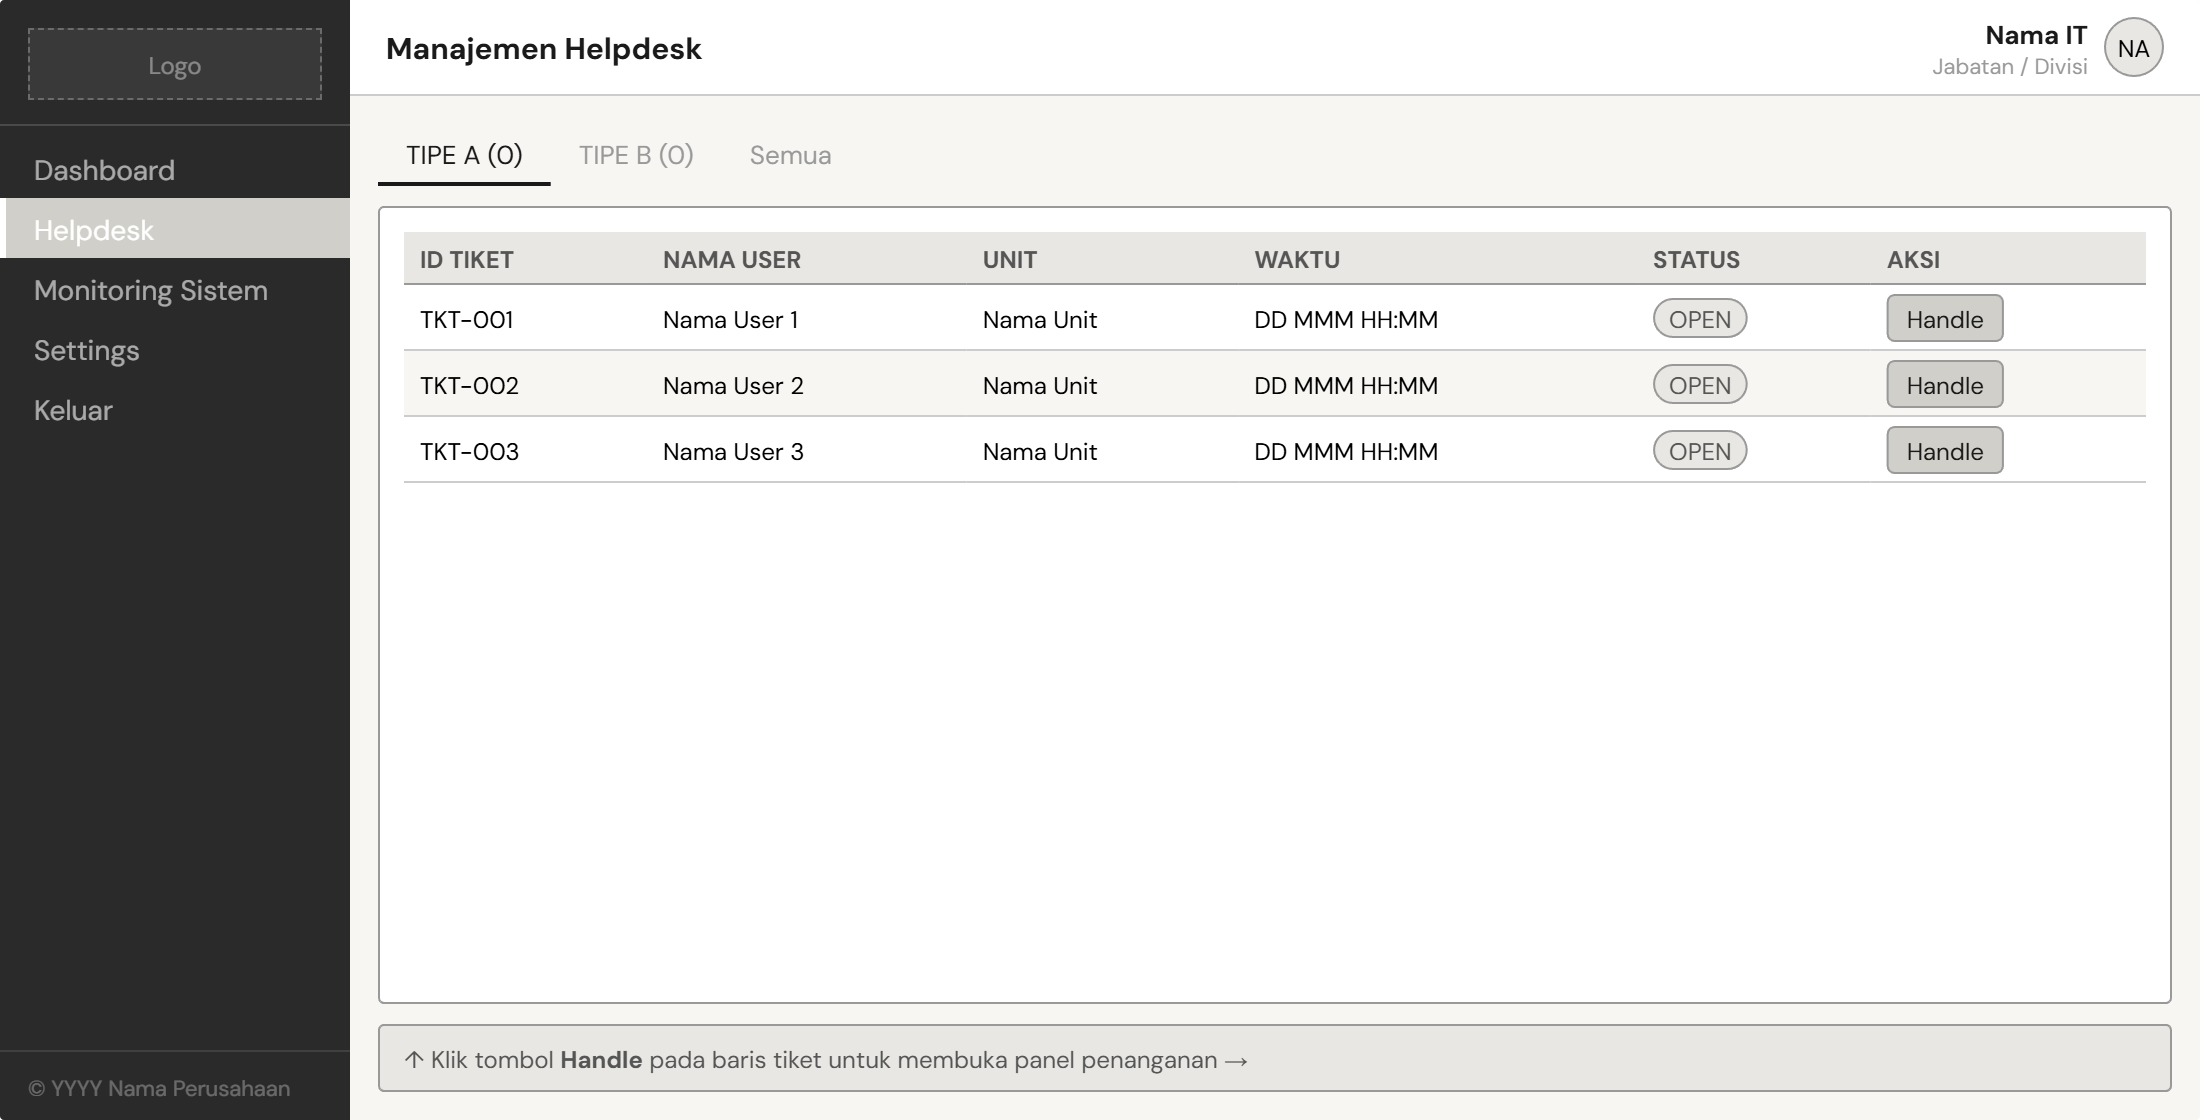
\includegraphics[width=0.85\textwidth]{figure/generated/lowfi-11a-helpdesk-daftar-tiket.png}
    \caption{Desain \textit{Mid Fidelity} Halaman Manajemen Helpdesk: Daftar Tiket}
    \label{fig:3.lofi-11a}
\end{figure}
Rancangan halaman manajemen helpdesk daftar tiket IT Support dapat dilihat pada Gambar \ref{fig:3.lofi-11a} diatas. Halaman manajemen helpdesk merupakan halaman kerja utama IT Support dalam mengelola seluruh tiket yang masuk, dengan sistem tab yang memisahkan tiket TOKEN, ISSUE, dan Semua. Halaman ini menampilkan tabel daftar tiket beserta status dan tombol Handle pada setiap baris untuk membuka panel penanganan tiket secara langsung. 


\textbf{20. Halaman Manajemen Helpdesk: Panel Handle Tiket TOKEN.} \par
Halaman ini menampilkan panel Handle yang muncul setelah IT Support menekan tombol Handle pada tiket TOKEN, memuat informasi lengkap pengaju tiket dan tombol Generate Token sebagai tindakan utama yang perlu dilakukan. Panel ini memungkinkan IT Support memproses tiket tanpa berpindah halaman, dengan panduan langkah yang ditampilkan secara jelas di dalam panel. Rancangan panel handle tiket TOKEN dapat dilihat pada Gambar \ref{fig:3.lofi-11b} berikut.

\begin{figure}[H]
    \centering
    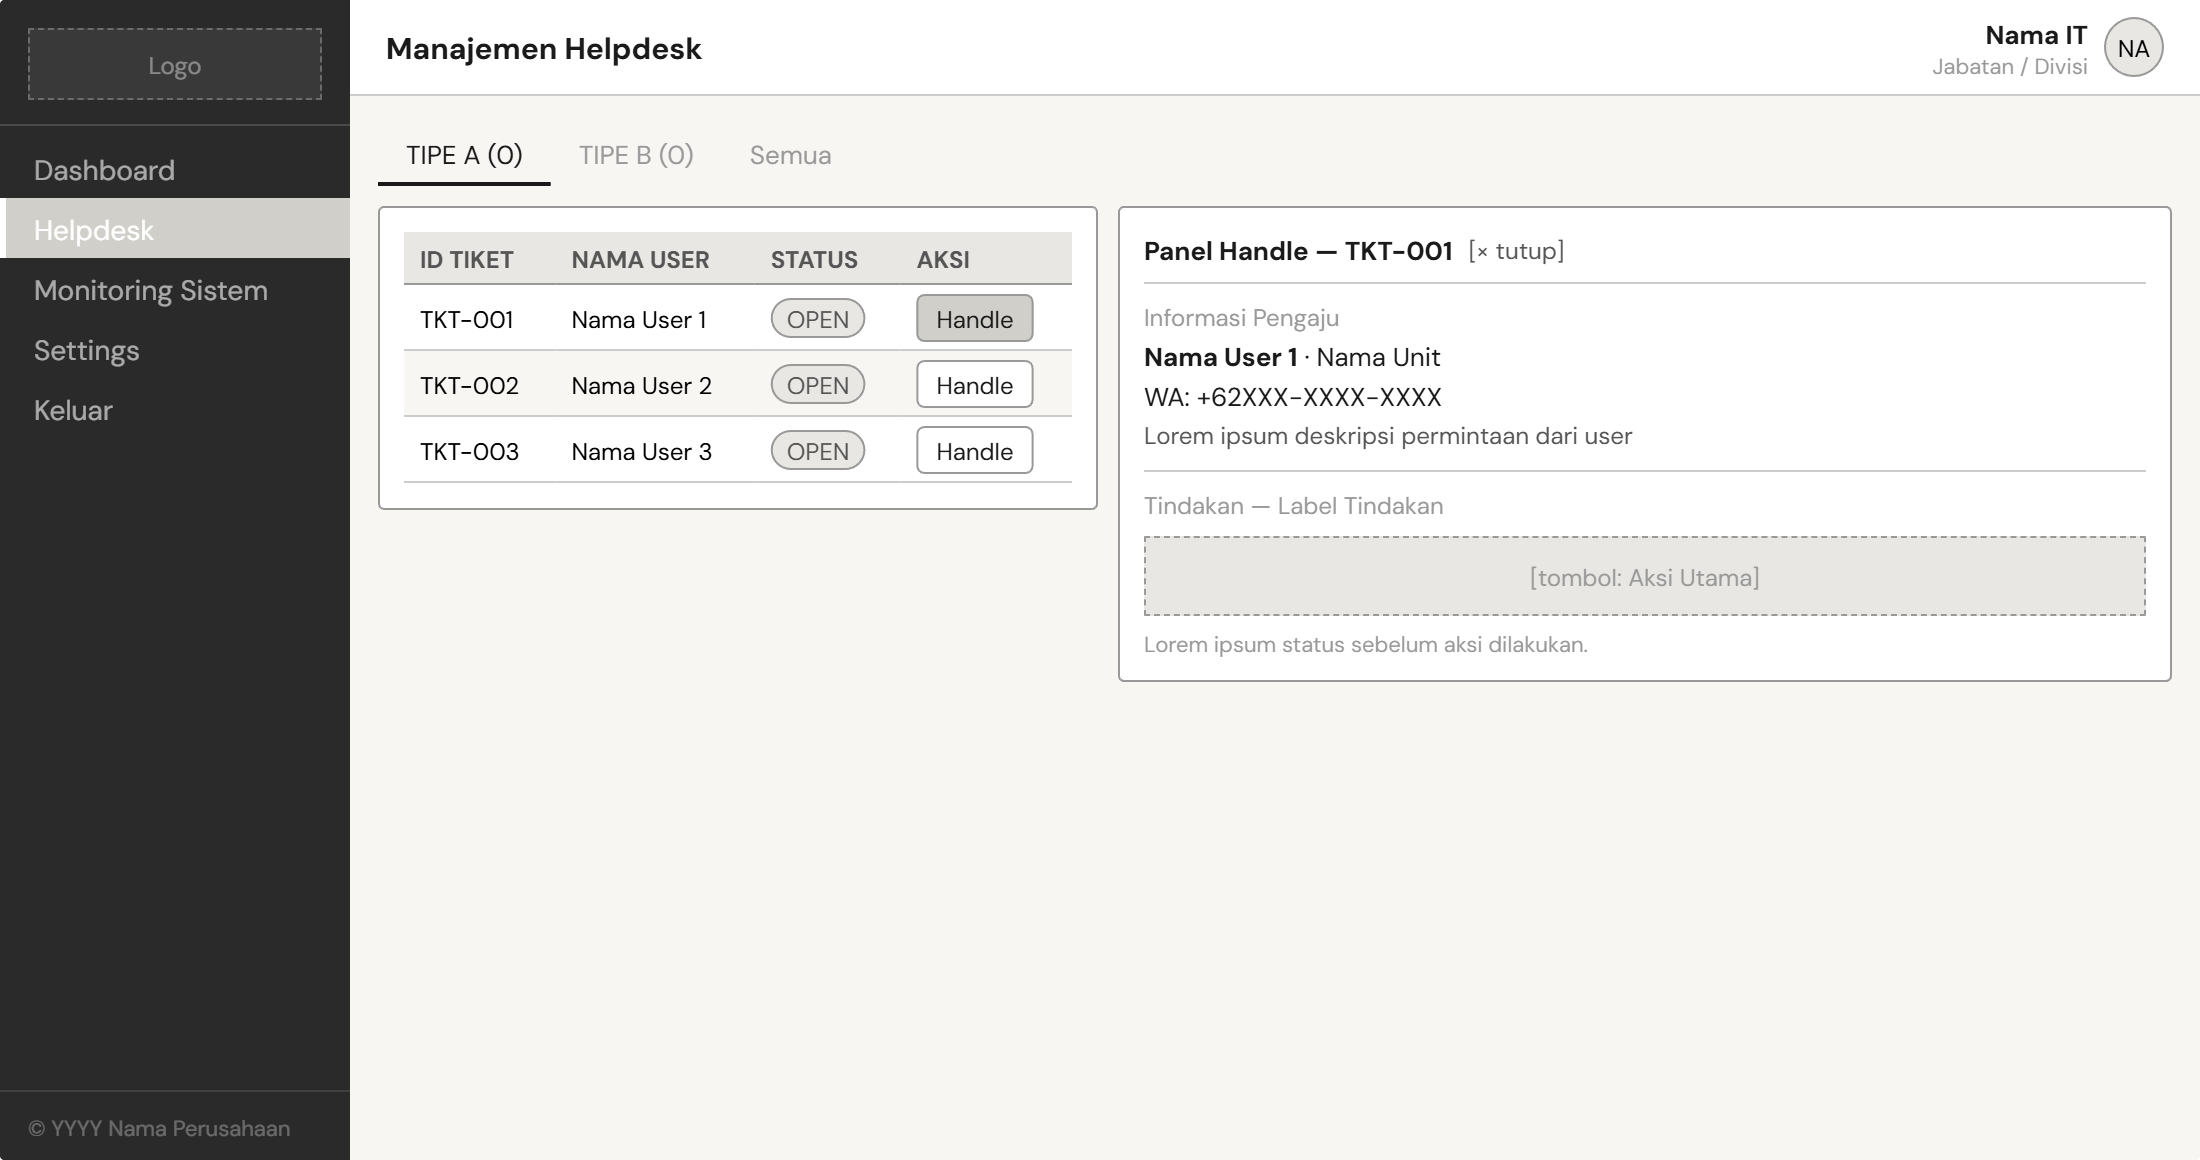
\includegraphics[width=0.85\textwidth]{figure/generated/lowfi-11b-helpdesk-panel-handle.png}
    \caption{Desain \textit{Mid Fidelity} Halaman Manajemen Helpdesk: Panel Handle Tiket TOKEN}
    \label{fig:3.lofi-11b}
\end{figure}

\textbf{21. Halaman Manajemen Helpdesk: Token Dibangkitkan \& Dikirim.} \par
Halaman ini menampilkan kondisi panel Handle setelah IT Support berhasil membangkitkan token, di mana token ditampilkan lengkap dengan masa berlakunya dan tombol Kirim via WhatsApp untuk mengirimkan token langsung ke pengguna. Setelah pengiriman berhasil, sistem menampilkan pesan konfirmasi dan IT Support dapat menutup tiket dengan menekan tombol Tandai Selesai \& Tutup. Rancangan panel handle tiket TOKEN setelah token dibangkitkan dan dikirim dapat dilihat pada Gambar \ref{fig:3.lofi-11c} berikut.

\begin{figure}[H]
    \centering
    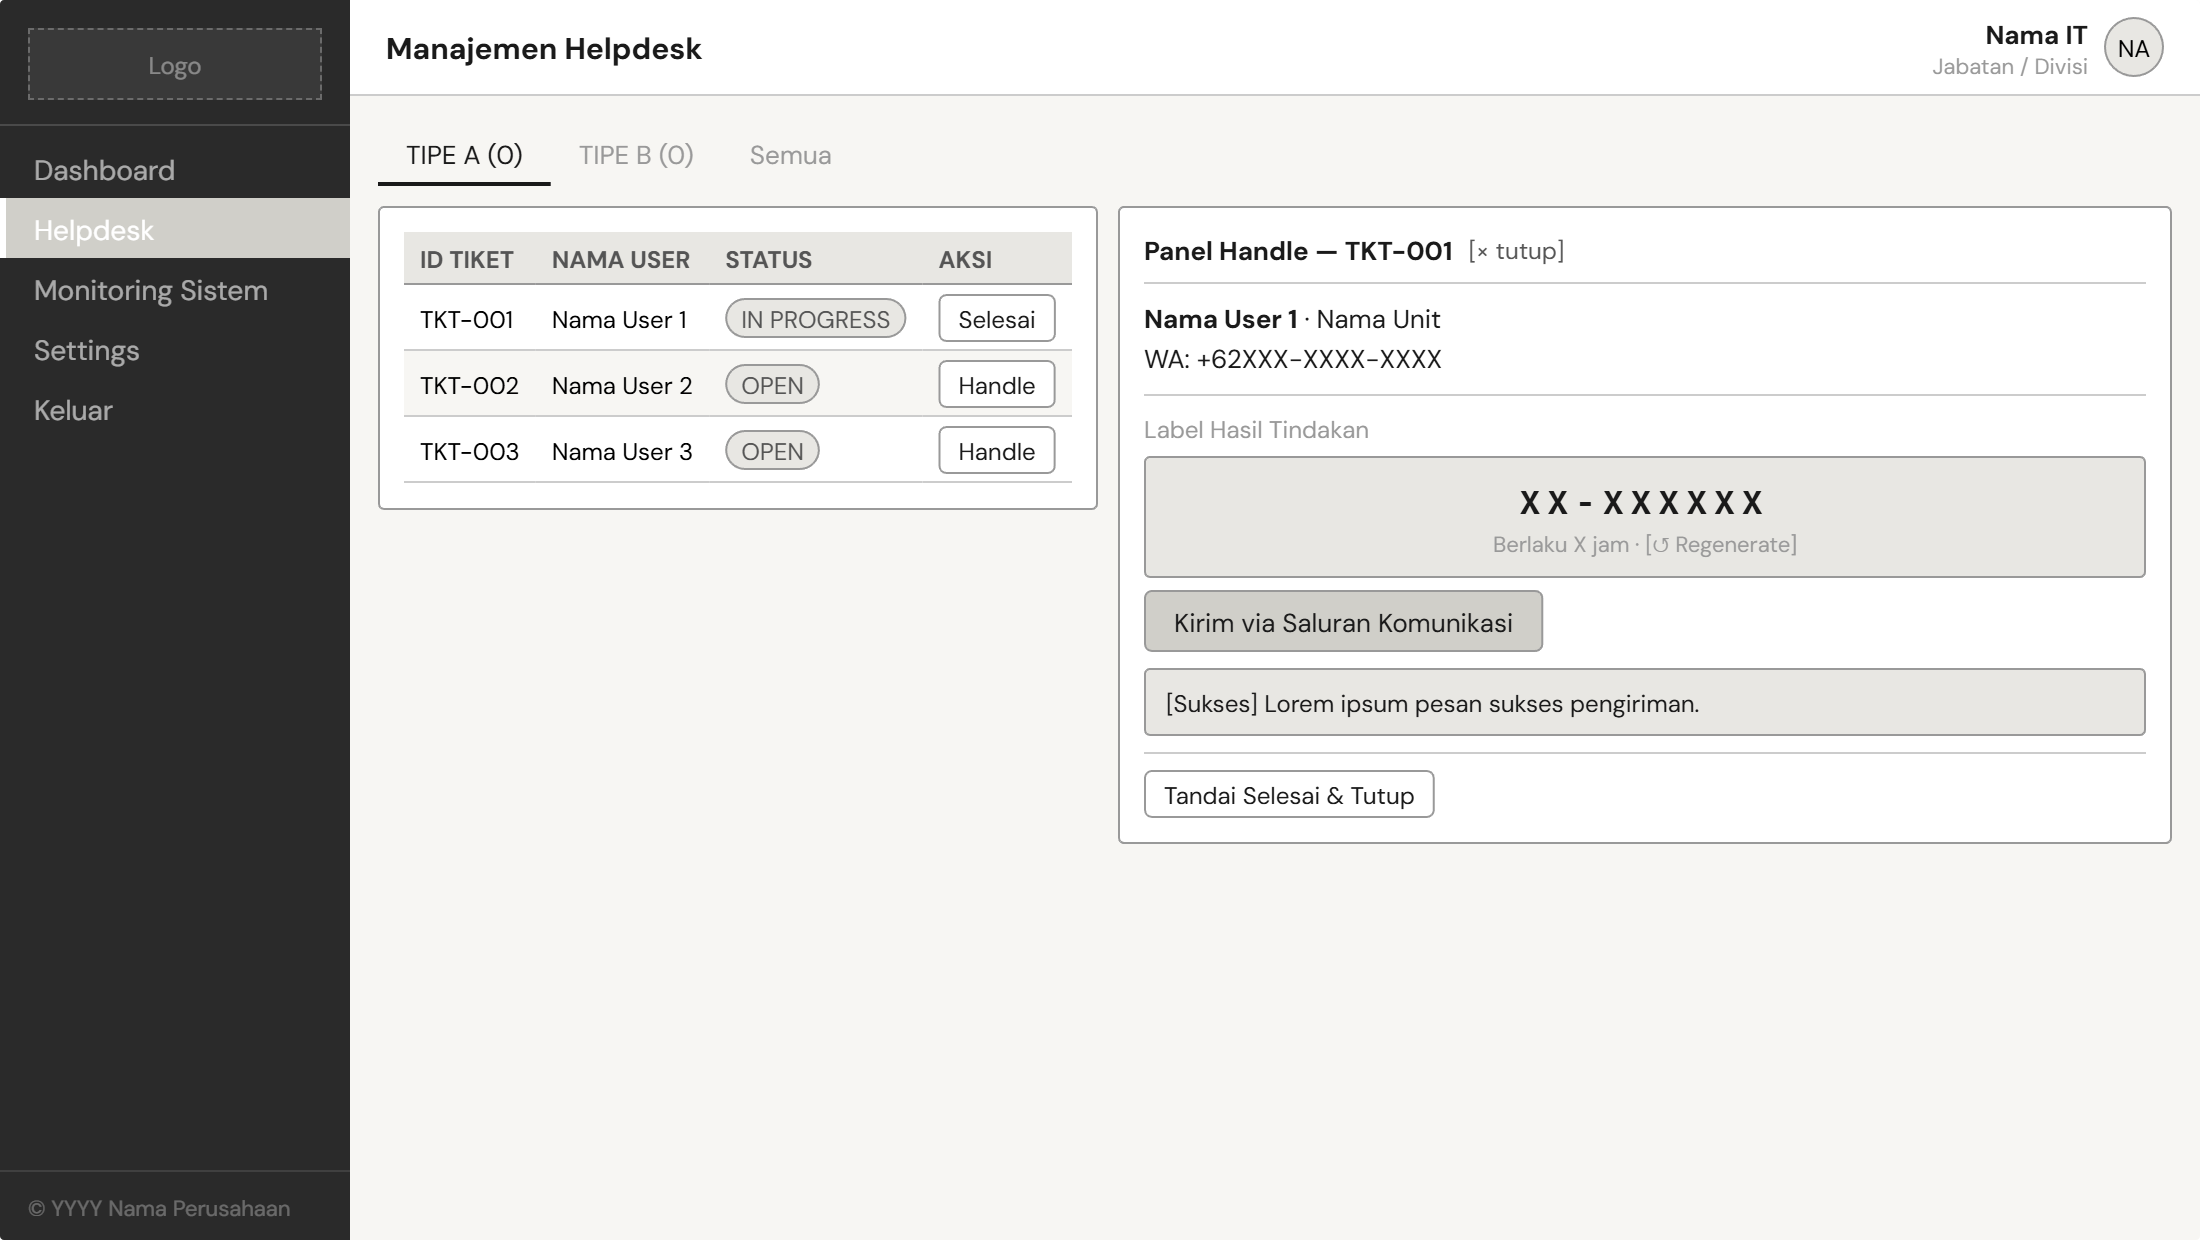
\includegraphics[width=0.85\textwidth]{figure/generated/lowfi-11c-helpdesk-token-kirim.png}
    \caption{Desain \textit{Mid Fidelity} Halaman Manajemen Helpdesk: Token Dibangkitkan \& Dikirim}
    \label{fig:3.lofi-11c}
\end{figure}

\subsection{Implementasi} \label{III.ImplDetail}
Pada tahap ini, peneliti mengimplementasikan rancangan sistem yang telah disetujui sebelumnya ke dalam bentuk program aplikasi yang dapat dijalankan. Peneliti mentransformasikan desain antarmuka, alur logika, serta struktur basis data ke dalam kode pemrograman sesuai dengan spesifikasi teknis yang telah ditetapkan pada tahap desain. Proses implementasi dilakukan secara bertahap dan modular, di mana setiap modul dikembangkan dan diuji secara mandiri sebelum diintegrasikan dengan modul lainnya. \par

Lingkungan pengembangan dibangun menggunakan sejumlah perangkat lunak yang telah ditetapkan pada Subbab \ref{III.Alat}. Sisi \textit{server} dikembangkan menggunakan Node.js dengan \textit{framework} Express.js untuk membangun dan mengelola \textit{Application Programming Interface} (API) sistem, sementara pengelolaan basis data MySQL ditangani melalui Prisma ORM. Sisi \textit{frontend} dibangun menggunakan React.js, komunikasi \textit{real-time} ditangani oleh Socket.io, dan integrasi WhatsApp menggunakan Baileys. Urutan implementasi mengikuti alur modular yang dimulai dari pengaturan skema basis data, modul autentikasi dan token, manajemen pengguna dan unit, laporan per jenis unit, validasi berlapis, \textit{helpdesk}, notifikasi, dasbor pemantauan, hingga ekspor laporan dalam format PDF dan Excel. \par

\subsection{Pengujian} \label{III.PengujianDetail}
Tahap pengujian dilakukan untuk memastikan bahwa sistem yang telah dibangun berjalan sesuai dengan kebutuhan yang telah ditetapkan dan dapat diterima oleh pengguna akhir. Pengujian pada penelitian ini menggunakan dua metode, yaitu \textit{black box testing} untuk memverifikasi fungsionalitas sistem dan \textit{User Acceptance Testing} (UAT) untuk mengukur tingkat keberterimaan sistem oleh pengguna \cite{abdillah2023blackbox}. Hasil pengujian menjadi dasar evaluasi apakah sistem layak untuk dirilis dan digunakan dalam lingkungan operasional nyata. \par

\subsubsection*{A. Blackbox Testing}
\textit{Black box testing} merupakan metode pengujian perangkat lunak yang berfokus pada verifikasi keluaran sistem terhadap masukan yang diberikan, tanpa memperhatikan struktur kode internal yang menjalankannya \cite{abdillah2023blackbox}. Metode ini digunakan untuk memastikan bahwa setiap fungsi yang telah diimplementasikan menghasilkan keluaran yang sesuai dengan kebutuhan fungsional yang telah ditetapkan sebelumnya. Pengujian dilakukan dengan mensimulasikan berbagai skenario penggunaan, baik skenario yang sesuai (positif) maupun skenario yang tidak sesuai (negatif), untuk memastikan sistem mampu menangani kedua kondisi tersebut dengan tepat. Detail skenario pengujian \textit{black box} disusun berdasarkan kebutuhan fungsional F-01 hingga F-12 yang telah dijabarkan pada Subbab \ref{III.AnalisKebutuhan}, sebagaimana ditunjukkan pada Tabel \ref{table:3.blackbox} berikut: \par

\begin{longtable}{|p{0.10\textwidth}|p{0.12\textwidth}|p{0.2\textwidth}|p{0.20\textwidth}|p{0.12\textwidth}|}
    \caption{Rancangan Skenario Blackbox Testing}
    \label{table:3.blackbox}\\
    \hline
    \textbf{Kode} & \textbf{Skenario} & \textbf{Deskripsi Pengujian} & \textbf{Hasil yang Diharapkan} & \textbf{Aktor} \\
    \hline
    \endfirsthead
    \multicolumn{5}{l}{\textit{Lanjutan dari halaman sebelumnya}} \\
    \caption[]{Rancangan Skenario Blackbox Testing} \\
    \hline
    \textbf{Kode} & \textbf{Skenario} & \textbf{Deskripsi Pengujian} & \textbf{Hasil yang Diharapkan} & \textbf{Aktor} \\
    \hline
    \endhead
    \hline
    \multicolumn{5}{r}{\textit{Bersambung ke halaman berikutnya}} \\
    \endfoot
    \endlastfoot
    F01-P1 & Login dengan kredensial valid & Login dengan \textit{username} dan \textit{password} yang benar & Berhasil masuk dan menampilkan \textit{dashboard} yang sesuai & User Unit, Admin Global, IT Support \\
    \hline
    F01-N1 & Login dengan \textit{username} tidak terdaftar & \textit{Username} tidak tersimpan di \textit{database} & Pesan error akses ditolak & User Unit, Admin Global, IT Support \\
    \hline
    F01-N2 & Login dengan \textit{password} salah & \textit{Username} benar, \textit{password} salah & Pesan error akses ditolak & User Unit, Admin Global, IT Support \\
    \hline
    F01-N3 & Akun terkunci ketika gagal login & Salah \textit{password} sebanyak 3 kali mencoba login ke sistem & Akun dikunci secara otomatis oleh sistem & User Unit / Admin Global / IT Support \\
    \hline
    F02-P1 & Input laporan dengan data wajib & User Unit mengisi seluruh data wajib laporan harian sesuai format unitnya & Laporan tersimpan ke dalam basis data dengan status DRAFT & User Unit \\
    \hline
    F02-P2 & Input laporan dengan \textit{box detail} & User Unit mengisi data wajib dan turut mengisi kolom \textit{box detail} opsional & Laporan tersimpan beserta data \textit{box detail} dengan status DRAFT & User Unit \\
    \hline
    F02-N1 & Input laporan dengan data tidak lengkap & User Unit mencoba menyimpan laporan tanpa mengisi salah satu atau lebih kolom wajib & Sistem menampilkan pesan kesalahan dan laporan tidak tersimpan & User Unit \\
    \hline
    F02-N2 & Input laporan kedua dalam satu hari & User Unit mencoba membuat laporan baru pada hari yang sama saat laporan sudah tersedia & Sistem menampilkan pesan bahwa laporan hari ini telah dibuat dan menghentikan proses & User Unit \\
    \hline
    F03-P1 & Validasi internal pada laporan lengkap & User Unit melakukan validasi pada laporan yang telah terisi lengkap dan benar & Status laporan berhasil berubah dari DRAFT menjadi \texttt{READY\allowbreak\_TO\allowbreak\_SUBMIT} & User Unit \\
    \hline
    F03-N1 & Validasi internal pada laporan tidak lengkap & User Unit mencoba melakukan validasi pada laporan yang masih memiliki kekurangan data & Status laporan berubah menjadi \texttt{NEED\allowbreak\_REVISION\allowbreak\_INTERNAL} dan meminta perbaikan & User Unit \\
    \hline
    F03-N2 & Validasi laporan milik unit lain & User Unit mencoba mengakses dan memvalidasi laporan milik unit lain & Sistem menolak akses dan menampilkan pesan bahwa laporan tidak dapat diakses & User Unit \\
    \hline
    F04-P1 & Submit laporan berstatus \texttt{READY\allowbreak\_TO\allowbreak\_SUBMIT} & User Unit menekan tombol \textit{submit} pada laporan yang berstatus \texttt{READY\allowbreak\_TO\allowbreak\_SUBMIT} & Status laporan berubah menjadi WAITING dan notifikasi \textit{real-time} dikirimkan ke Admin Global & User Unit \\
    \hline
    F04-N1 & Submit laporan berstatus bukan \texttt{READY\allowbreak\_TO\allowbreak\_SUBMIT} & User Unit mencoba menekan tombol \textit{submit} pada laporan yang tidak berstatus \texttt{READY\allowbreak\_TO\allowbreak\_SUBMIT} & Sistem menolak proses dan menampilkan pesan bahwa laporan belum siap di-\textit{submit} & User Unit \\
    \hline
    F05-P1 & Review laporan ACC & Admin Global memberikan keputusan ACC pada laporan yang masuk & Status laporan berubah menjadi ACC, dicatat di AuditLog, dan notifikasi \textit{real-time} dikirim ke User Unit & Admin Global \\
    \hline
    F05-P2 & Review laporan REVISI & Admin Global memberikan keputusan REVISI disertai catatan & Status laporan berubah menjadi REVISI, dicatat di AuditLog, notifikasi WhatsApp dan \textit{real-time} dikirim ke User Unit & Admin Global \\
    \hline
    F06-P1 & Dashboard Admin Global & Admin Global membuka halaman \textit{dashboard} & Sistem menampilkan status pemantauan dan data seluruh unit secara \textit{real-time} & Admin Global \\
    \hline
    F06-P2 & Dashboard User Unit & User Unit membuka halaman \textit{dashboard} & Sistem menampilkan status dan data laporan milik unit pengguna yang sedang \textit{login} & User Unit \\
    \hline
    F06-N1 & User Unit mengakses data unit lain & User Unit mencoba mengakses data laporan yang berbeda dari unitnya melalui \textit{dashboard} & Sistem menolak akses dan hanya menampilkan data milik unit pengguna yang bersangkutan & User Unit \\
    \hline
    F07-P1 & Notifikasi \textit{real-time} laporan di-REVISI & Admin Global menetapkan status REVISI pada laporan & User Unit menerima notifikasi \textit{real-time} dalam sistem secara langsung & User Unit \\
    \hline
    F07-P2 & Notifikasi WhatsApp laporan di-REVISI & Admin Global menetapkan status REVISI pada laporan & Pesan notifikasi terkirim ke nomor WhatsApp User Unit terkait melalui Baileys & User Unit \\
    \hline
    F07-P3 & Notifikasi WhatsApp \textit{helpdesk} REVISION masuk & User Unit mengajukan \textit{helpdesk} jenis REVISION & Admin Global menerima notifikasi WhatsApp bahwa terdapat permintaan revisi laporan yang masuk & Admin Global \\
    \hline
    F08-P1 & Pengajuan \textit{helpdesk} TOKEN & User Unit atau Admin Global mengajukan tiket \textit{helpdesk} jenis TOKEN dengan mengisi deskripsi kendala & Tiket tersimpan dan notifikasi WhatsApp dikirimkan ke IT Support untuk ditindaklanjuti & User Unit / Admin Global \\
    \hline
    F08-P2 & Pengajuan \textit{helpdesk} ISSUE & User Unit mengajukan tiket \textit{helpdesk} jenis ISSUE dengan mengisi deskripsi kendala & Tiket tersimpan dan notifikasi WhatsApp dikirimkan ke IT Support untuk ditindaklanjuti & User Unit \\
    \hline
    F08-P3 & Pengajuan \textit{helpdesk} REVISION & User Unit mengajukan tiket \textit{helpdesk} jenis REVISION terkait laporan yang ingin diubah & Tiket tersimpan dan notifikasi WhatsApp dikirimkan ke Admin Global untuk ditindaklanjuti & User Unit \\
    \hline
    F08-N1 & Pengajuan \textit{helpdesk} tanpa deskripsi & User Unit mencoba mengirimkan tiket \textit{helpdesk} dengan kolom deskripsi yang masih kosong & Sistem menampilkan pesan kesalahan dan tiket tidak tersimpan & User Unit \\
    \hline
    F09-P1 & Admin Global membuat akun pengguna & Admin Global mengisi formulir pembuatan akun baru pengguna & Akun pengguna baru tersimpan dalam sistem & Admin Global \\
    \hline
    F09-P2 & Admin Global mengedit data akun pengguna & Admin Global mengubah data akun pengguna yang sudah terdaftar & Data akun berhasil diperbarui dalam sistem & Admin Global \\
    \hline
    F09-P3 & Admin Global menonaktifkan akun pengguna & Admin Global menonaktifkan akun pengguna yang sudah tidak aktif & Akun berhasil dinonaktifkan dan pengguna tidak dapat masuk ke sistem & Admin Global \\
    \hline
    F09-P4 & Admin Global mengelola data unit & Admin Global menambahkan atau mengubah data unit kerja dalam sistem & Data unit berhasil tersimpan dan dapat digunakan sebagai referensi laporan & Admin Global \\
    \hline
    F10-P1 & IT Support \textit{generate} token & IT Support memproses tiket TOKEN dan membangkitkan token \textit{reset password} & Token \textit{one-time} berhasil dibangkitkan dan dikirimkan ke nomor WhatsApp pengguna & IT Support \\
    \hline
    F10-P2 & IT Support menyelesaikan tiket TOKEN & Token berhasil digunakan oleh pengguna untuk melakukan \textit{reset password} & Status tiket TOKEN berubah menjadi RESOLVED secara otomatis & IT Support \\
    \hline
    F10-N1 & Token \textit{generate} untuk akun tidak terkunci & IT Support mencoba membangkitkan token untuk akun yang tidak dalam kondisi terkunci & Sistem menolak proses dan menampilkan pesan bahwa akun tidak memerlukan \textit{reset password} & IT Support \\
    \hline
    F10-N2 & Token kedaluwarsa sebelum digunakan & Pengguna mencoba menggunakan token yang sudah melewati batas waktu satu jam & Sistem menolak token dan menampilkan pesan token tidak valid atau kedaluwarsa & User Unit \\
    \hline
    F10-N3 & Token digunakan lebih dari satu kali & Pengguna mencoba menggunakan token yang sudah pernah dipakai sebelumnya & Sistem menolak permintaan dan menampilkan pesan token sudah tidak berlaku & User Unit \\
    \hline
    F11-P1 & Audit log tercatat & Admin Global melakukan keputusan ACC atau REVISI terhadap laporan & Aktivitas tercatat secara otomatis dalam AuditLog dengan informasi lengkap & Admin Global \\
    \hline
    F11-P2 & Admin Global melihat riwayat audit log & Admin Global membuka halaman riwayat aktivitas sistem & Sistem menampilkan daftar seluruh aktivitas yang telah tercatat beserta informasi aktor, waktu, dan detail tindakan & Admin Global \\
    \hline
    F11-P3 & Audit log mencatat aktivitas \textit{helpdesk} & IT Support atau Admin Global menyelesaikan tiket \textit{helpdesk} & Aktivitas penanganan \textit{helpdesk} tercatat secara otomatis dalam AuditLog & IT Support / Admin Global \\
    \hline
    F12-P1 & Input target periode & User Unit mengisi data target kinerja per periode & Target tersimpan dan dapat digunakan sebagai perbandingan dengan realisasi & User Unit \\
    \hline
\end{longtable}

\subsubsection*{B. User Acceptance Testing (UAT)}
\textit{User Acceptance Testing} (UAT) dilakukan untuk mengukur tingkat keberterimaan sistem oleh pengguna akhir berdasarkan standar ISO/IEC 25010 \cite{lamada2024iso}. Pengujian ini melibatkan pengguna langsung dari unit-unit terkait di PT KAI Divre I Sumatera Utara. Aspek-aspek yang diuji mencakup enam karakteristik kualitas ISO/IEC 25010, yaitu Keamanan (\textit{Security}), Kinerja (\textit{Performance Efficiency}), Kemudahan Penggunaan (\textit{Usability}), Keandalan (\textit{Reliability}), Kompatibilitas (\textit{Compatibility}), dan Ketersediaan (\textit{Availability}) \cite{lamada2024iso}. Instrumen kuesioner menggunakan skala Likert 1–5 dengan kriteria penilaian sebagai berikut: (1) Sangat Tidak Setuju, (2) Tidak Setuju, (3) Netral, (4) Setuju, dan (5) Sangat Setuju. Hasil rata-rata skor per aspek kemudian dikonversi menjadi persentase untuk menentukan tingkat keberterimaan sistem. Rancangan kuesioner UAT berdasarkan standar ISO/IEC 25010 dapat dilihat pada Tabel \ref{table:3.uat} berikut: \par

\begin{longtable}{|p{0.05\textwidth}|p{0.18\textwidth}|p{0.47\textwidth}|p{0.18\textwidth}|}
    \caption{Rancangan Kuesioner UAT Berdasarkan ISO/IEC 25010}
    \label{table:3.uat}\\
    \hline
    \textbf{No} & \textbf{Karakteristik ISO/IEC 25010} & \textbf{Pernyataan} & \textbf{Responden} \\
    \hline
    \endfirsthead
    \multicolumn{4}{l}{\textit{Lanjutan dari halaman sebelumnya}} \\
    \caption[]{Rancangan Kuesioner UAT Berdasarkan ISO/IEC 25010} \\
    \hline
    \textbf{No} & \textbf{Karakteristik ISO/IEC 25010} & \textbf{Pernyataan} & \textbf{Responden} \\
    \hline
    \endhead
    \hline
    \multicolumn{4}{r}{\textit{Bersambung ke halaman berikutnya}} \\
    \endfoot
    \endlastfoot
    1 & \multirow{5}{=}{Keamanan} & Sistem hanya dapat diakses oleh pengguna yang telah memiliki akun terdaftar & User Unit / Admin Global / IT Support \\
    \cline{1-1}\cline{3-4}
    2 & & Saya tidak dapat mengakses fitur atau data yang bukan menjadi wewenang peran saya & User Unit / Admin Global / IT Support \\
    \cline{1-1}\cline{3-4}
    3 & & Sistem mengunci akun secara otomatis setelah tiga kali percobaan login yang gagal & User Unit / Admin Global / IT Support \\
    \cline{1-1}\cline{3-4}
    4 & & Proses pemulihan akun melalui token yang dikirimkan via WhatsApp terasa aman dan terkontrol & User Unit / IT Support \\
    \cline{1-1}\cline{3-4}
    5 & & Saya merasa data laporan yang saya \textit{input} terlindungi dan tidak dapat diubah oleh pihak lain tanpa izin & User Unit / Admin Global \\
    \hline
    6 & \multirow{4}{=}{Kinerja} & Sistem menampilkan data dan halaman dengan cepat tanpa penundaan yang mengganggu & User Unit / Admin Global / IT Support \\
    \cline{1-1}\cline{3-4}
    7 & & Notifikasi \textit{real-time} terkait perubahan status laporan diterima tanpa jeda waktu yang lama & User Unit / Admin Global \\
    \cline{1-1}\cline{3-4}
    8 & & Sistem tetap berjalan dengan baik meskipun digunakan secara bersamaan oleh beberapa pengguna & User Unit / Admin Global / IT Support \\
    \cline{1-1}\cline{3-4}
    9 & & Proses \textit{submit} laporan dan pembaruan status berlangsung dengan cepat setelah tombol ditekan & User Unit / Admin Global \\
    \hline
    10 & \multirow{6}{=}{Kemudahan Penggunaan} & Tampilan antarmuka sistem mudah dipahami tanpa memerlukan pelatihan khusus sebelumnya & User Unit / Admin Global / IT Support \\
    \cline{1-1}\cline{3-4}
    11 & & Saya dapat menemukan fitur yang saya butuhkan dengan mudah di dalam sistem & User Unit / Admin Global / IT Support \\
    \cline{1-1}\cline{3-4}
    12 & & Proses penginputan laporan harian dapat dilakukan dengan mudah dan tidak membingungkan & User Unit \\
    \cline{1-1}\cline{3-4}
    13 & & Alur pengajuan \textit{helpdesk} mudah diikuti dan tidak memerlukan langkah yang berlebihan & User Unit \\
    \cline{1-1}\cline{3-4}
    14 & & Proses peninjauan dan pemberian keputusan laporan (ACC/REVISI) dapat dilakukan dengan mudah melalui \textit{dashboard} & Admin Global \\
    \cline{1-1}\cline{3-4}
    15 & & Proses penanganan tiket \textit{helpdesk} dan pembangkitan token \textit{reset password} mudah dilakukan di dalam sistem & IT Support \\
    \hline
    16 & \multirow{4}{=}{Keandalan} & Sistem berjalan stabil dan tidak mengalami gangguan saat saya menggunakannya & User Unit / Admin Global / IT Support \\
    \cline{1-1}\cline{3-4}
    17 & & Data laporan yang telah saya simpan tidak hilang atau berubah tanpa alasan yang jelas & User Unit / Admin Global \\
    \cline{1-1}\cline{3-4}
    18 & & Sistem mampu menangani kesalahan \textit{input} dengan baik dan menampilkan pesan yang informatif & User Unit / Admin Global / IT Support \\
    \cline{1-1}\cline{3-4}
    19 & & Notifikasi WhatsApp terkait status laporan dan \textit{helpdesk} selalu terkirim dengan benar & User Unit / Admin Global / IT Support \\
    \hline
    20 & \multirow{3}{=}{Kompatibilitas} & Sistem dapat diakses dan digunakan dengan baik melalui \textit{browser} yang biasa saya gunakan & User Unit / Admin Global / IT Support \\
    \cline{1-1}\cline{3-4}
    21 & & Tampilan sistem tetap dapat dibaca dan digunakan dengan baik di perangkat yang saya miliki & User Unit / Admin Global / IT Support \\
    \cline{1-1}\cline{3-4}
    22 & & Tidak ada fitur sistem yang gagal berfungsi akibat perbedaan perangkat atau \textit{browser} yang digunakan & User Unit / Admin Global / IT Support \\
    \hline
    23 & \multirow{3}{=}{Ketersediaan} & Sistem dapat diakses kapan saja selama perangkat saya terhubung dengan jaringan internet & User Unit / Admin Global / IT Support \\
    \cline{1-1}\cline{3-4}
    24 & & Saya tidak pernah mengalami kondisi sistem tidak dapat diakses sama sekali saat saya membutuhkannya & User Unit / Admin Global / IT Support \\
    \cline{1-1}\cline{3-4}
    25 & & Sistem tersedia dan siap digunakan pada jam kerja operasional tanpa hambatan & User Unit / Admin Global / IT Support \\
    \hline
\end{longtable}

\subsection{Perilisan dan Pemeliharaan} \label{III.Perilisan2}
Tahap perilisan merupakan tahap di mana sistem yang telah dinyatakan layak melalui proses pengujian mulai dioperasikan secara resmi dalam lingkungan kerja nyata di PT KAI Divre I Sumatera Utara. Sebelum sistem dioperasikan sepenuhnya, dilakukan serangkaian persiapan akhir yang mencakup konfigurasi \textit{server}, pengaturan akun pengguna awal, serta pengecekan ulang seluruh koneksi layanan eksternal seperti WhatsApp Gateway melalui Baileys dan komunikasi \textit{real-time} melalui Socket.io. Proses peralihan dari sistem lama yang berbasis grup WhatsApp ke sistem baru dilakukan secara terencana agar tidak mengganggu kelangsungan proses pelaporan harian yang sudah berjalan. \par

Setelah sistem resmi dirilis, tahap pemeliharaan dimulai sebagai upaya untuk menjaga kestabilan dan keandalan sistem dalam jangka panjang. Pemeliharaan dilakukan secara berkala oleh IT Support yang bertugas memantau kondisi sistem, menangani kendala teknis yang muncul, serta memastikan seluruh layanan berjalan sesuai yang diharapkan. Apabila ditemukan kesalahan atau ketidaksesuaian fungsi setelah sistem dioperasikan, perbaikan dilakukan dengan merujuk kembali pada rancangan yang telah dibuat tanpa harus mengulang keseluruhan proses pengembangan dari awal. Pendekatan ini selaras dengan karakteristik metode \textit{Modified Waterfall} yang memungkinkan adanya penyesuaian pada tahap tertentu tanpa mengganggu tahapan lain yang telah selesai. \par

Pemeliharaan sistem juga mencakup pembaruan data dan konfigurasi yang diperlukan seiring berkembangnya kebutuhan operasional PT KAI Divre I Sumatera Utara di masa mendatang. Karena sistem dirancang dengan pendekatan modular, setiap komponen dapat diperbarui atau diperluas secara mandiri tanpa memengaruhi komponen lain yang sedang berjalan. Hal ini memberikan fleksibilitas bagi tim IT untuk mengembangkan sistem lebih lanjut, misalnya dengan menambahkan unit pelaporan baru atau memperluas fitur notifikasi sesuai kebutuhan bisnis yang terus berkembang \cite{prasnowo2024waterfall}. \par
